\documentclass{article}

% ========== PACKAGES ==========================================================
\usepackage{graphicx}
\usepackage{amsmath}

\usepackage{verbatim}
% to type multi-line comments

\usepackage[margin=2cm]{geometry} 
% used to reduce page margins

\usepackage{xspace} 
% to add spaces after personalized commands

\usepackage{wrapfig}
% to allign vertically images and text

\usepackage{enumitem}

\usepackage{amssymb}
\usepackage{amsmath}
\usepackage[dvipsnames]{xcolor}
\usepackage{ragged2e}
\usepackage{subcaption} % to make subfigures
\usepackage{caption} % to extend caption's length

\usepackage{silence} % to silence overflow warnings
\usepackage{sectsty}
\usepackage{mathtools}

% ========== PERSNALIZED COMMANDS ==============================================
\newcommand{\expect}{\mathbb{E}}
\newcommand{\real}{\mathbb{R}}
\newcommand{\prob}{\mathbb{P}}
\newcommand{\ssigma}{$\sigma$\xspace}
\newcommand{\diff}{$\neq$\xspace}
\newcommand{\arrow}{$\rightarrow$\xspace}
\newcommand{\seps}{$\varepsilon$\xspace}
\newcommand{\testset}{$\mathcal{D}_{test}$\xspace}
\newcommand{\dataset}{$\mathcal{D}$\xspace}


% ========== PERSNALIZED EASTETIC ==============================================
\definecolor{sec-color}{RGB}{255, 133, 51}
\sectionfont{\color{sec-color}}
\definecolor{subsec-color}{RGB}{51, 102, 255}
\subsectionfont{\color{subsec-color}}
\definecolor{subsubsec-color}{RGB}{102, 179, 255}
\subsubsectionfont{\color{subsubsec-color}}


% ========== HEADER ============================================================
\title{062102 - Applied Statistics}
\author{Guflie}


\graphicspath{ {img/} }

\begin{document}
% ========== DOC ===============================================================
\centering

\includegraphics[width=10cm]{polimi_logo.pdf}

\vspace{2.5cm}
{\huge \textbf{062102 - Applied Statistics} \\}

\vspace{0.5cm}
{\Large Polytechnic University of Milan \\}

\vspace{0.3cm}
{\large A.Y. 2025/26 \textit{class notes} \\}

\raggedright
\vspace{7cm}
{\large Authors}: Guflie \\
\vspace{0.2cm}
{\large Professor}: Massi Michela Carlotta \\
\newpage

\tableofcontents
\newpage

\section{Introduction}

Statistic is the foundation for all data-driven decision-making processes, also
in the AI era: in fact, nowdays machine learning models rely mostly on statistical
methods. The main difference resides in the purpose: \textit{ML models} are designed to 
make the most accurate prediction possible, \textit{statistical models} instead aim to 
make inference about the relationship between the data.
\begin{figure}[h]
    \centering
    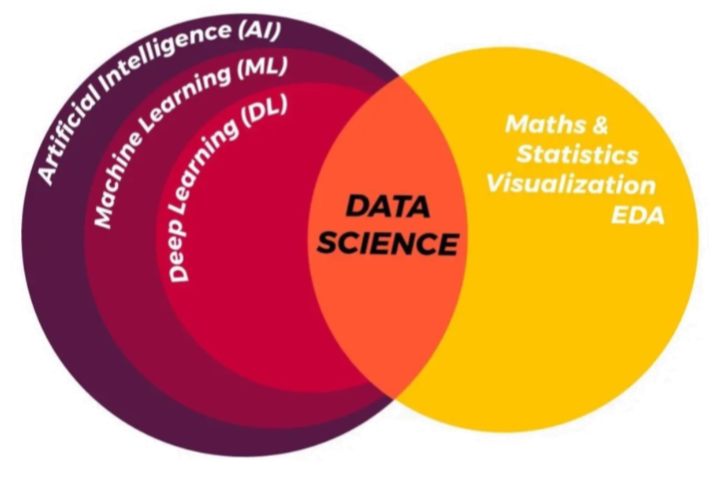
\includegraphics[width=0.3\textwidth]{introduction/ml_statistic_intersection.png}
\end{figure}

In this course we are going to deal with \textit{multivariated data}, meaning that each 
datapoint contains several variables, defining its \textit{dimensions}. Representing this data 
with matrices is the more convient way.
\begin{figure}[h]
    \centering
    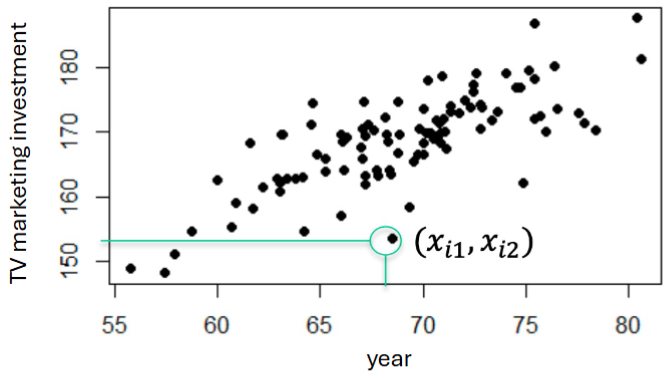
\includegraphics[width=0.3\textwidth]{introduction/multivariated_data_example.png}
\end{figure}

\vspace{1cm}

As for ML, we have different classes of methods based on the available data and how we 
interpret them:
\begin{description}[itemsep=0.6cm]
    \item[Supervised learning] \hfill \\
    \begin{minipage}{0.9\textwidth}
        \begin{wrapfigure}{l}{0.3\textwidth}
            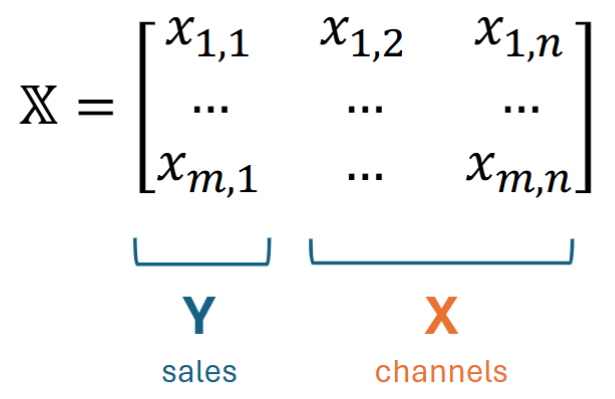
\includegraphics[width=0.25\textwidth]{introduction/target_feature_relationship.png}
        \end{wrapfigure}
        \hfill \\
        In this class we can identify a \textbf{target} variable $Y$ and a set of "input"
        variables $X$ called \textbf{features}.  Targets and features relationship is
        expressed trougth a function affected by a certain error $\varepsilon$: 
        $Y=f(X)+\varepsilon$. The error $\varepsilon$ is something we can never get rid of
        it, we should think about it as a property of the data.\\
        Typically in this set of method we try to make predictions about new target values or 
        to find those features that are more important to explain the targets.
    \end{minipage}
    
    \item[Unsupervised learning] \hfill \\
    \begin{minipage}{0.9\textwidth}
        \begin{wrapfigure}{l}{0.3\textwidth}
            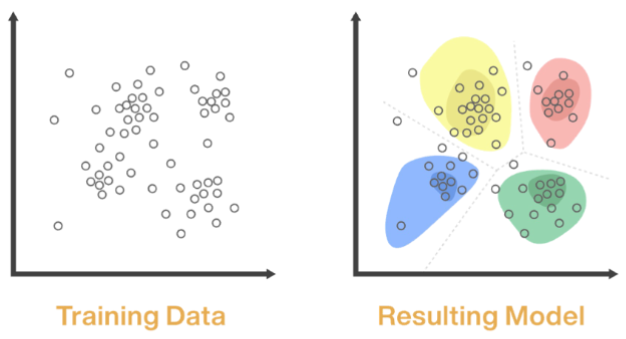
\includegraphics[width=0.25\textwidth]{introduction/example_unsupervised.png}
        \end{wrapfigure}
        \hfill \\
        In this case there aren't target variables, but all the variables are features 
        ($f(X)\approx X$). \\ This set of models focuses on exploiting structures and patterns
        within the data itself.
    \end{minipage}
\end{description}
\vspace{0.8cm}

\begin{figure}[t]
    \centering
    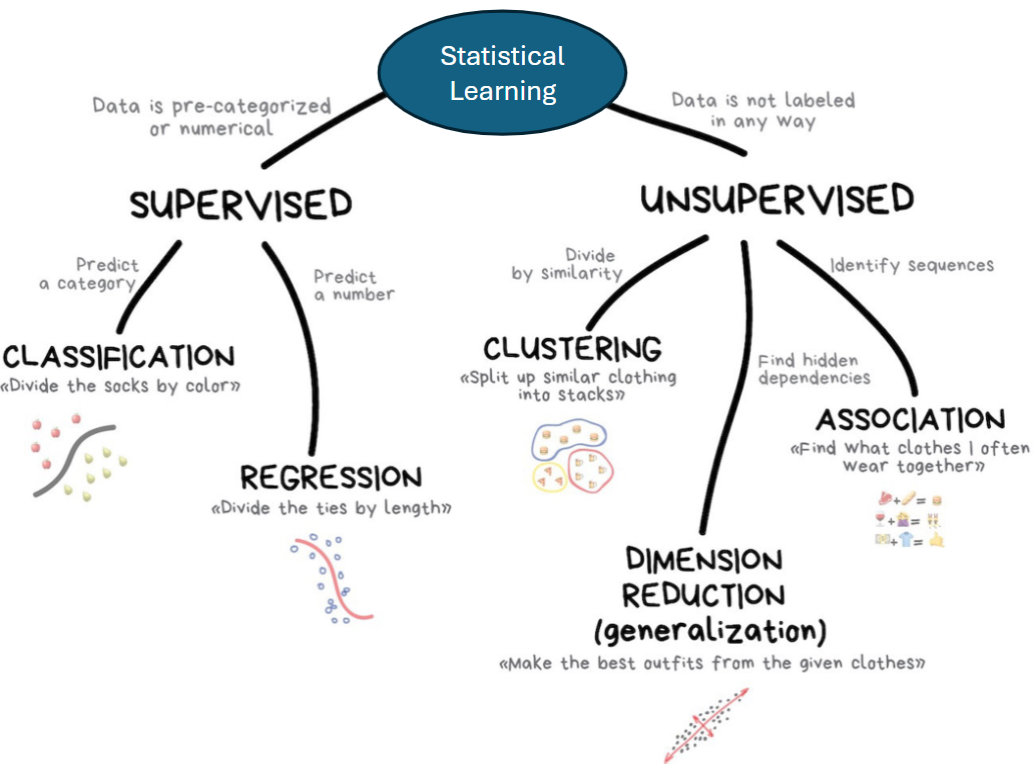
\includegraphics[width=0.6\textwidth]{introduction/methods_taxonomy.png}
    \caption{Taxionomy of the methods explored during the course.}
\end{figure}
\newpage

\subsection{Model goodness}
How do we find a good model for our data? \\
To start, let's take linear models as examples, like $Y=\beta_0 x_0 + \beta_1 x_1 \dots + 
\beta_p x_p$. \\
The models we want to use are expressed through a set of \textbf{parameters} of our choice
(in the previous example we have $p+1$ parameters); the goal is to tune these parameters
using training data in order to shape our function accordingly to the data. However most 
of the times linear models are not complex enough, and we have to shift toward more complex 
ones.
\begin{figure}[h]
    \centering
    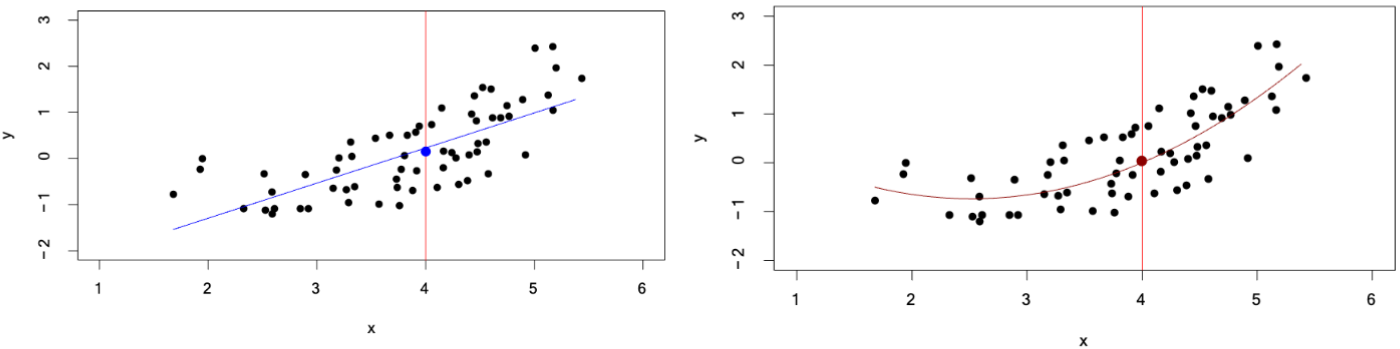
\includegraphics[width=0.65\textwidth]{introduction/linear_quadratic_models_comparison.png}
    \caption{Comparison between linear model ($f(X)=\beta_o + \beta_1 x$) and quadratic 
    model ($f(X)= \beta_0 + \beta_1 x +\beta_2 x^2$).}
\end{figure}

Usually the choice of a model is influenced by some trade-offs:
\begin{itemize}
    \item \textit{prediction accuracy vs interpretability} : we might trade-off the model's
    accuracy to make it more interpretable
    \item \textit{parsimony principle} : usually we prefer simpler models involving fewer
    variables since they're easier to manage
    \item \textit{good fit vs over-fit or under-fit } : see below
\end{itemize}
\newpage

\subsection{Underfitting vs Overfitting problem}

Start with the example of estimating the height of the next student entering the room 
during lecture, in order to do that our prediction $\hat{y}$ should minimize a certain 
function, usually the \textbf{Mean Squared prediction Error (MSE)}.
\begin{equation*}
    MSE(\hat{y})=\frac{1}{n}\sum_{i=1}^n (\hat{y}_i-y_i)^2
\end{equation*}

If we know the height of all students, we want to use the population mean $\mu$ as 
predictor, doing so we get as MSE $\mathbb{E}[(Y-\mu)^2]=Var(Y)=\sigma^2$.\\
\begin{center} \textcolor{red}{
    \textbf{The data variance is irreducible, we can't do better than that.}   
} \end{center}
\hfill \\

However, it's impossible to have information about the whole population; so what we do
is taking a small sample from it over and over, using the sample mean $\bar{Y}$ as $\mu$
and getting $MSE_{avg}=\mathbb{E}[(\hat{Y}-Y)^2]$. By decomposing the average MSE we are
able to understand which are our sources of error: this reduction leads to two source of
errors, \textit{bias} and \textit{variance}.
\begin{description}
    \item[Bias]: $Bias(\hat{Y})=\expect[\hat{Y}-\mu]$, we have bias if our predictions 
    are systematically to high or too low
    \item[Variance]: $Var(\hat{Y})=\expect[(\hat{Y}-\expect[\hat{Y}])^2]$ , we have
    high variance if our predictions are very sensitive on the sampling we draw from 
    the universe
\end{description}
\begin{figure}[h]
    \centering
    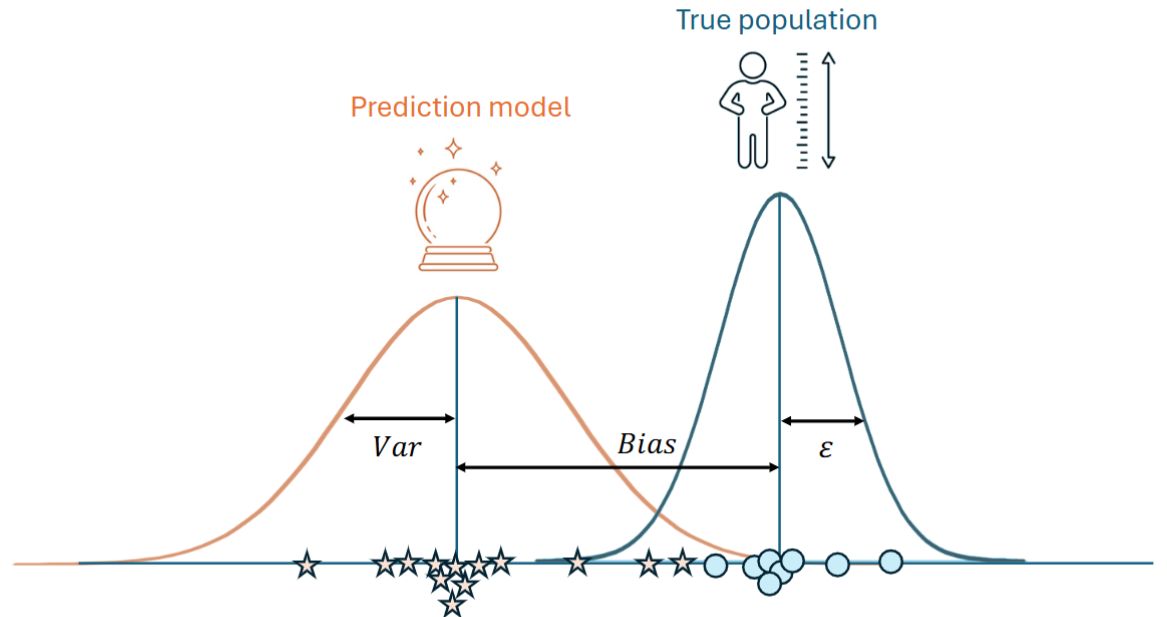
\includegraphics[width=0.6\textwidth]{introduction/bias_variance_idea.png}
\end{figure}

So if we try to fit a model $f(X)$ with some training data, and we end up with $\hat{f}(X)$
with some test observation $(x_0,y_0)$, we have that
\begin{equation*}
    \expect[y_0-\hat{f}(x_0)] = Var[\hat{f}(x_0)] + Bias[\hat{f}(x_0)]^2 + Var(\varepsilon)
\end{equation*}
\begin{description}
    \item[Variance]: captures how much our model changes based on the training dataset
    \item[Bias]: the inherent error we get from our models
    \item[Noise]: ambiguity due the data distribution   
\end{description}
\newpage

If we take a model too much simple, we end up with something having high bias, but not really
susceptible to training set (low variance) $\Rightarrow$ \textbf{Underfitting}.
\begin{figure}[h]
    \centering
    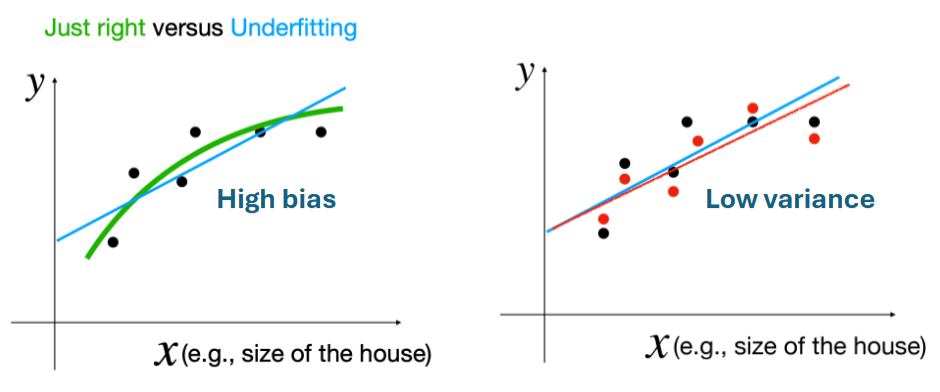
\includegraphics[width=0.6\textwidth]{introduction/underfitting.png}
\end{figure}

If instead we use a model too complex we get something with very low bias, but extrimelly
sensitive to the data we sample $\Rightarrow$ \textbf{Overfitting}.
\begin{figure}[h]
    \centering
    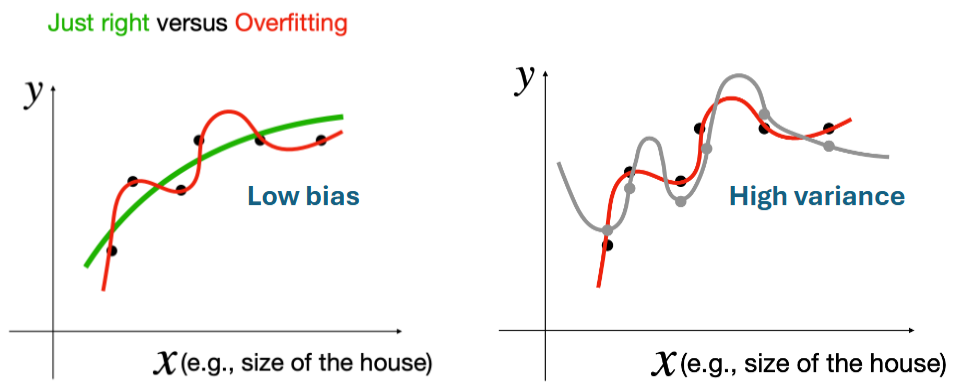
\includegraphics[width=0.6\textwidth]{introduction/overfitting.png}
\end{figure}

What we see in practise is that Bias and Variance are strictly correlated: while one of the
two decreases, the other increases. This force us to find some trade-off between these twos.
\begin{figure}[h]
    \centering
    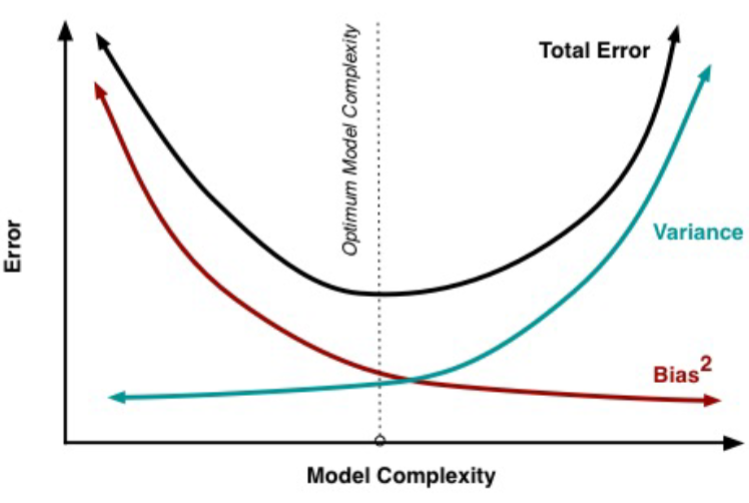
\includegraphics[width=0.6\textwidth]{introduction/tradeoff_bias_variance.png}
\end{figure}

\section{Dimensionality reduction}

When dealing with big data (also not very big) we'll always clash with the
\textbf{Curse of dimensionality}:
\begin{center}
    \textit{In applied mathematics, curse of dimensionality refers to the problem 
    caused by the exponential increase in volume associated with adding extra 
    dimensions to a mathematical space.}
\end{center}
\vspace{0.7cm}

Let's look at the \textbf{example} of categorizing some bacteria:
\begin{figure}[h]
    \centering
    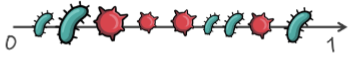
\includegraphics[width=0.3\textwidth]{dr/example_cd_1d.png}
\end{figure}

To separate the groups better we add new information about another measure
\textcolor{gray}{(before we have that each point has one feature, while now 
we're considering two features for each point, if you think about it you are 
in fact adding information and making the points more different from each other)}
\begin{figure}[h]
    \centering
    \begin{subfigure}[t]{0.2\textwidth}
        \centering
        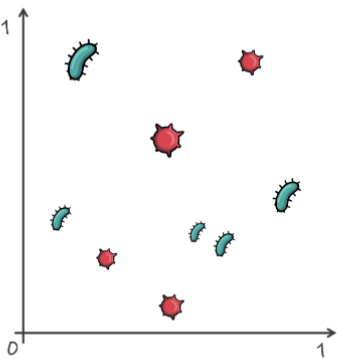
\includegraphics[width=0.95\linewidth]{dr/example_cd_2d.png}
    \end{subfigure}
    \hspace{0.5cm}
    \begin{subfigure}[t]{0.2\textwidth}
        \centering
        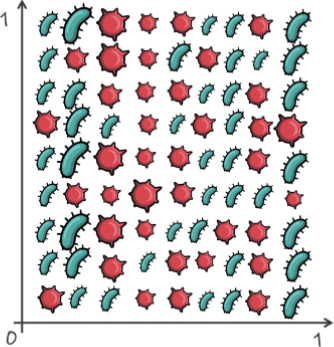
\includegraphics[width=0.95\linewidth]{dr/example_cd_2d_expl.png}
        {
            \captionsetup{width=1.5\linewidth, margin={0cm, -3cm}, labelformat=empty}
            \caption{If we try to maintain for the 2-d scenario the same density of 
            the 1-dimension case, we would end up with 81 samples.}
        }
    \end{subfigure}
\end{figure}

If we extend the space up to the 3th dimension we are capable of 
distinguish the data using only a linear model. To do the same in 2 dimensions
we should have used more complex models.
\begin{figure}[h]
    \centering
    \begin{subfigure}[t]{0.3\textwidth}
        \centering
        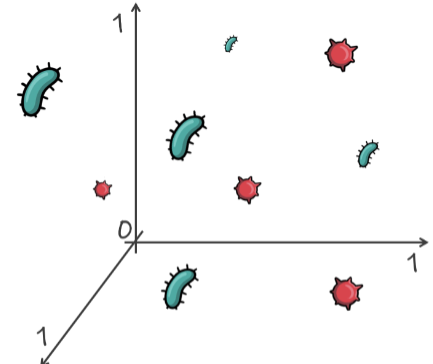
\includegraphics[width=0.9\linewidth]{dr/example_cd_3d.png}
    \end{subfigure}
    \hspace{0.2cm}
    \begin{subfigure}[t]{0.3\textwidth}
        \centering
        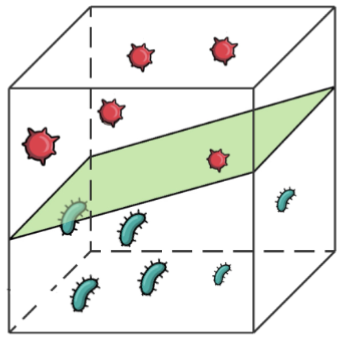
\includegraphics[width=0.9\linewidth]{dr/example_3d_divison.png}
    \end{subfigure}    
\end{figure}

\newpage
Another phenomena of the curse of dimensionality is \textbf{Distance concentration}: as 
the number of samples goes to infinity, the relative distances between point tend to 
become zero, starting to concetrate on the expected value.
\begin{figure}[h]
    \centering
    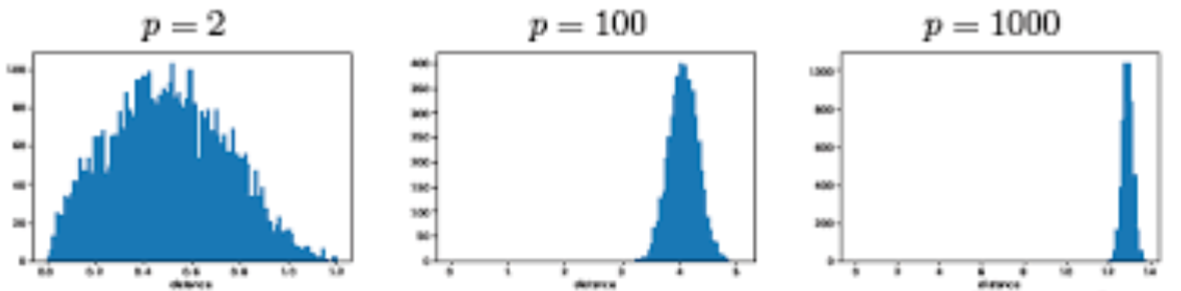
\includegraphics[width=0.7\textwidth]{dr/distance_concentration.png}
\end{figure}

\vspace{2cm}
\subsection{Principal Component Analysis (PCA)}

What if we have $n$ data points, $p$ features and $n<p$ ?
It means that some fatures might look something completely different, but in 
reality some of them are just a combination of others $\rightarrow$ we 
have \textbf{collinear features}.
Collinear features make harder our job of understanding how each feature influences
the targets : let's assume that $x_1$ and $x_2$ are collinear
\begin{equation}
    y = \beta_0 + \beta_1 x_1 + \beta_2 x_2 +\varepsilon
\end{equation}
due collinearity, we can't see the individual effect of $x_1$ and $x_2$ on $y$.
%\vspace{0.8cm}

\begin{figure}[h]
    \centering
    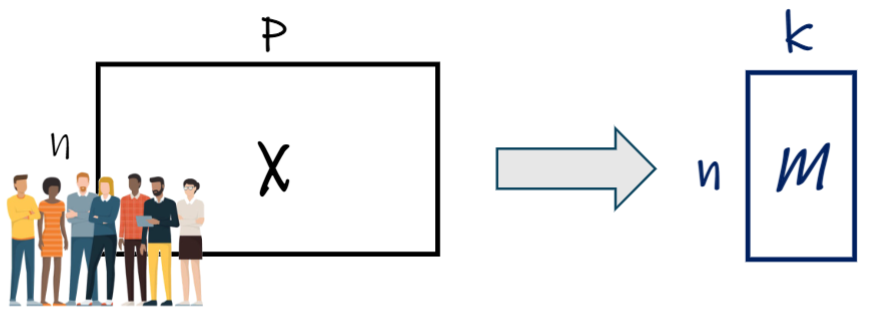
\includegraphics[width=0.5\textwidth]{dr/pca/dr_matrix_example.png}    
\end{figure}
What we want to do is to summarize the data having $p$ features with the smaller
set ok $k$ artifically derived features; to do this we must balance the clarity of
representation and the loss of information due the compression $\Rightarrow$ 
\textbf{Principal Component Analysis (PCA)} aims to do this using linear 
combinations of the selected variables.

\vspace{0.6cm}
\textcolor{Green}{\textbf{Example}:}\\
Imagine that we want to describe our blood cells sample, and the initial 
features are \textit{diameter} and \textit{thickness}, how can we reduce
the number of features?
\begin{figure}[h]
    \centering    
    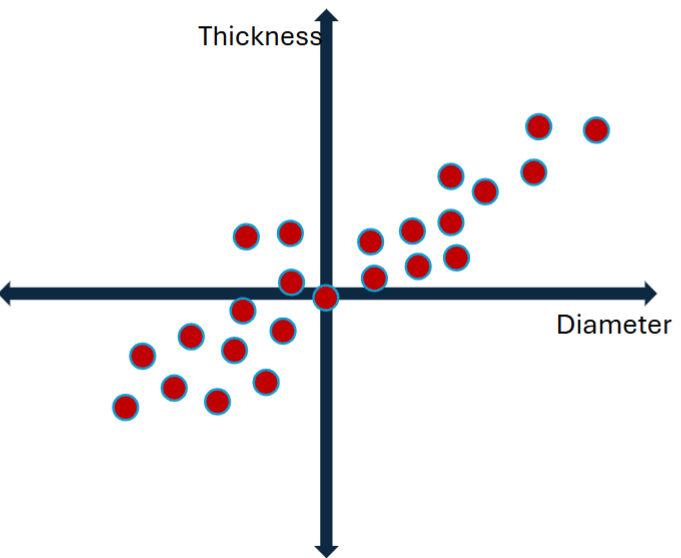
\includegraphics[width=0.3\textwidth]{dr/pca/blood_cells.png}
\end{figure}
\newpage

We can think of projecting the points along one of the two dimensions, choosing it
based on how spreaded the data are along it (e.g. so preserving more information).
\begin{center} \textcolor{red}{
    \textbf{In statitics information = variability.}   
} \end{center}
\begin{figure} [h]
    \centering
    \begin{subfigure}[c]{0.25\textwidth}
        \centering
        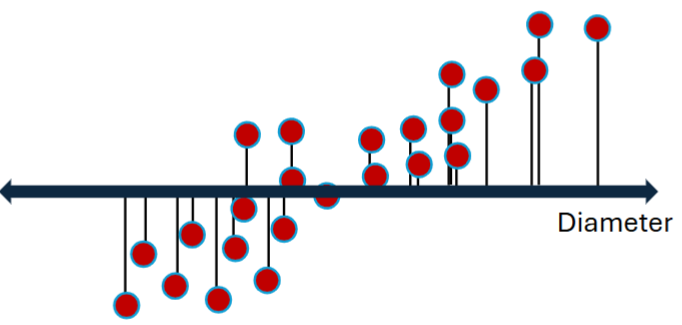
\includegraphics[width=\linewidth]{dr/pca/dr_blood_ex1.png}
    \end{subfigure}
    \hspace{1cm}
    \begin{subfigure}[c]{0.2\textwidth}
        \centering
        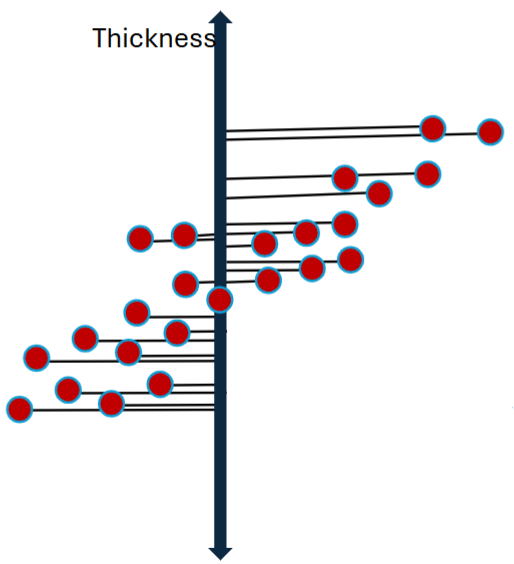
\includegraphics[width=\linewidth]{dr/pca/dr_blood_ex2.png}
    \end{subfigure}
\end{figure}

So we need a way to capture the maximal variability of the data: in other
words to find \textit{along which dimension the data spread the most}.
\begin{figure}[h]
    \centering
    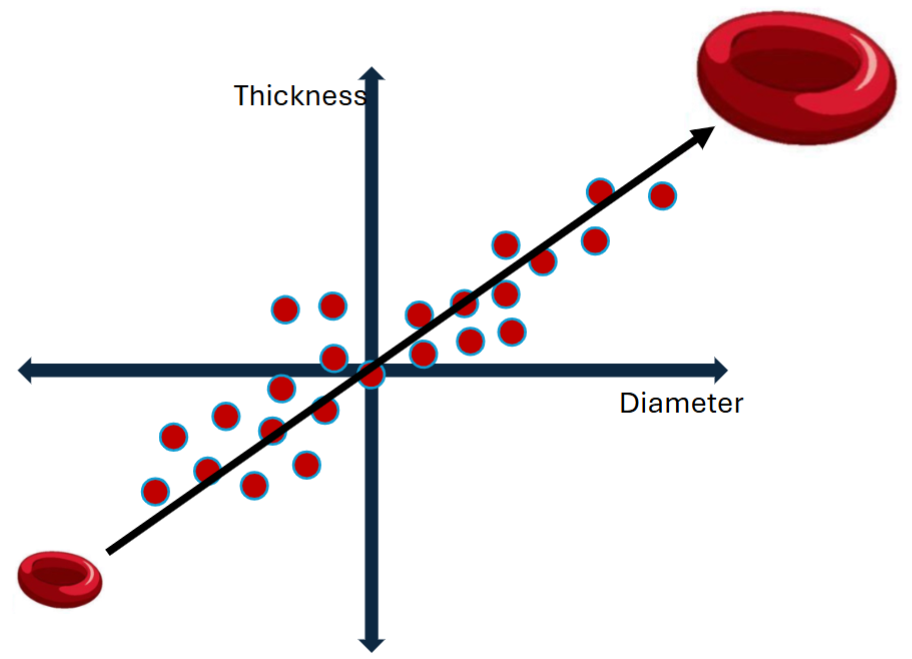
\includegraphics[width=0.3\textwidth]{dr/pca/pca_maxvar_example.png}
\end{figure}

PCA's goal is to project the data along those directions of maximal variability,
ending up with a new reference system for the data points \textcolor{gray}{(it's 
nothing different from vector space rotations, in 2D you visualize it by immaging
that the axis rotate)}.\\
\hfill \\

This objective can be expressed in two equivalent ways:
\begin{description}
    \item[Maximize variance]: maximize the data spread along that
    direction
    \item[Minimize residuals]: minimize the distance of the data points
    from the the dimension
\end{description}
\begin{figure}[h]
    \centering
    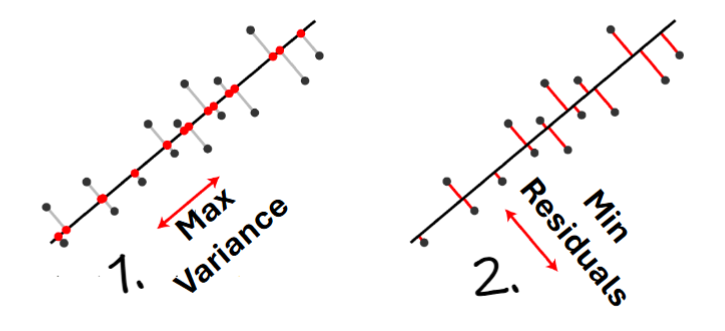
\includegraphics[width=0.45\textwidth]{dr/pca/pca_goal_visualzed.png}
\end{figure}

In order to do the PCA:
\begin{enumerate}
    \item get a set of data points $x^{(1)}\dots x^{(n)}\in \real^p$
    \item center the data in $(0,0)$ if needed: $x^{(i)}\leftarrow x^{(i)}-
    \bar{x}$
    \item choose a direction $u\in\real^p\ :\ \|x\|_2=1$
    \item project the data $x^{(i)}$ on $u$ : $z_i = u^Tx^{(i)}\in \real$
\end{enumerate}

Taking the objective of maximizing the variance, we observe that since the data are 
centered (avg = 0), the varince is:
\begin{equation*}
    Var(z) = \frac{1}{n}\sum_{i=1}^n z_i^2 = \frac{1}{n}\sum_{i=1}^n 
    (u^Tx^{(i)})^2 = 0
    \ \rightarrow\ 
    \max_{u\in\real^p}\frac{1}{n}\sum_{i=1}^n (u^Tx^{(i)})^2
\end{equation*}
if we define the \textit{empirical covariance matrix} as
\begin{equation*}
    \Sigma = \frac{1}{n}\sum_{i=1}^n x^{(i)}x^{(i)T} \ \in 
    \real^{p\times p}
\end{equation*}
we get that
\begin{equation*}
    \frac{1}{n}\sum_{i=1}^n (u^Tx^{(i)})^2 = u^T(\frac{1}{n}
    \sum_{i=1}^n x^{(i)}x^{(i)T})u = u^T\Sigma u
    \rightarrow
    \max_{u\in\real^p} u^T\Sigma u
\end{equation*}
The constraint on $u$ can be expressed as $u^Tu=1$ (turning constraint into 
an equation)

By switching to the Lagrangian relaxed problem:
\begin{equation*}
    \mathcal{L}(u,\lambda)=u^T\Sigma u-\lambda(u^Tu-1)
\end{equation*}

and taking the derivative
\begin{equation*}
    \nabla_u (u^T\Sigma u) = 2\Sigma u,\ \nabla_u (u^Tu) = 2u
    \Rightarrow \nabla_u \mathcal(L) = 2\Sigma u-2\lambda u = 0
    \Rightarrow \Sigma u = \lambda u
\end{equation*}

$\Rightarrow$ a candidate direction $u$ must be an \textbf{eigenvector of $\mathbf{\Sigma}$}.\\
So the objective function becomes $u^T\Sigma u=u^T (\lambda u) = \lambda
(u^T u) = \lambda \rightarrow$ by choosing the highest $\lambda$ we get the
highest objective function. So as principal component we take the eigenvector with the highest 
eigenvalue. If we want more dimension, we take also the second, the third ... \\
\hfill \\

We can interpret $\Sigma$ so that, when applied to the data
modifies the shape, it strech them toward their principal component, which 
are the $\Sigma$'s eigenvectors.
\begin{figure}[h]
    \centering
    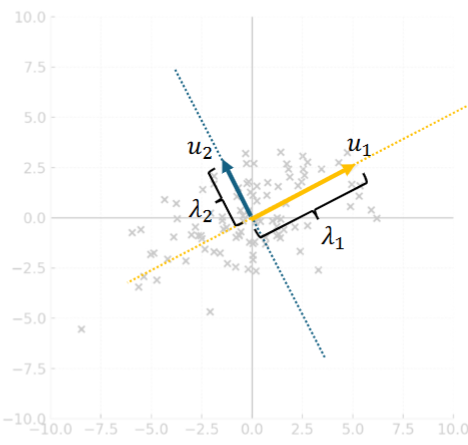
\includegraphics[width=0.3\textwidth]{dr/pca/covmat_projection.png}
\end{figure}

Two nice properties of PCA are:
\begin{enumerate}
    \item PCA results are rotation-invariant (depend only on the data, not 
    on the starting axis)
    \item PCs are independent/uncorrelated from each other by construction (they are eigenvectors)
\end{enumerate}

\newpage
\subsubsection{Express data with PCA's components}
We can see that the original observations can be re-written using the new
components: given the starting dimensions $\langle x_1\dots x_p \rangle$, we 
have
\begin{equation*}
    PC_j = \phi_{j1}x_1 \dots + \phi_{jp}x_p \Rightarrow z_{ij} = \phi_{1j}x_{i1}
    \dots + \phi_{pj}x_{ip}
\end{equation*}
where $z_{i,j}$ is the projection of $x^{(i)}$ on the $PC_j$ called \textbf{score}
and $\phi_{1j},\dots \phi_{pj}$ are the \textbf{weights} given to each original 
feature to translate it into the new PCA coordinates system. 
\begin{figure}[h]
    \centering
    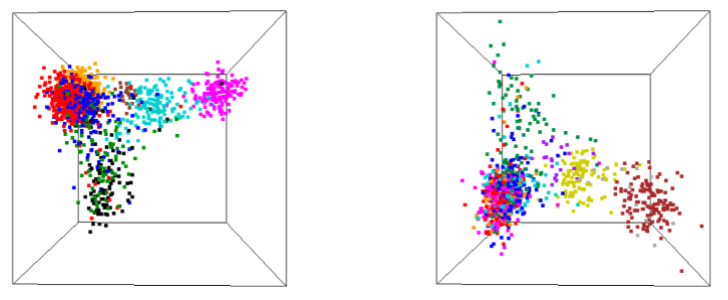
\includegraphics[width=0.7\textwidth]{dr/pca/pca_projection_example.png}
\end{figure}

\hfill \\
Note: standardization ($x-\mu/\sigma$) address the problem of
high-variance features dominating principal components.
\vspace{0.5cm}


\textbf{Why this stuff is useful other than re-shaping the data?}\\
Usually the data variability depends only on a small subset of all $p$ features, 
so we can use these to have a $k$-low-dimensional/compressed representation of 
the dataset. The choice of $k$ is the trade-off.

\subsubsection{Portion of Variance Explained}
We would like to quantify how much each singular Principal Component (PC)
explains the data variability.
\begin{equation*}
    Var_{\scriptscriptstyle TOT}= \sum_{j=1}^p Var(x_j) = \sum_{j=1}^p \left(\frac{1}{n}\sum_{i=1}^n x_{ij}^2\right)
\end{equation*}
If we name $Var_k$ := variance explained by the single k-th PC and $Var_{exp}$ := the
portion of Variance Explained by the selected first $k$ components
\begin{equation*}
    Var_k = \frac{1}{n}\sum_{i=1}^n z_{ik}^2 \Rightarrow Var_{exp} = \cfrac
    {\sum_k Var_k}{Var_{\scriptscriptstyle TOT}}
\end{equation*}
However, since the PCs are the eigenvalues of $\Sigma$:
\begin{equation*}
    Var_k = \frac{1}{n}\sum_{i=1}^n z_{ik}^2 = u_k^T\Sigma u_k = u_k^T(\lambda_k
    u_k) = \lambda_k
\end{equation*}
\begin{equation*}
    Var_{\scriptscriptstyle TOT} = \sum_{j=1}^p Var(x_j) = tr(\Sigma) = \sum_{j=1}^p \lambda_k
\end{equation*}
So we can define:
\begin{description}
    \item[$\mathbf{EVR_k}$ Explained Variance Ratio of $\mathbf{k}$] = $\cfrac{\lambda_k}
    {\sum_{m=1}p}\lambda_m$
    \item[$\mathbf{CumEV(K)}$ Cumulative Explained Variance] of the $K$ selection of
    component = $\cfrac{\sum_{k=1}^K\lambda_k}{\sum_{m=1}p}\ \lambda_m$   
\end{description}

\newpage
Depending on how much variability we'd like to retain, we can module the number
of dimensions in $K$ based on the \textit{CumEV index}.
This technique can be used also to other purposes, not only to tune the variance
level: it can be used also to set the data noise treshold to remove those components which 
"make too much noise".
\begin{figure}[h]
    \centering
    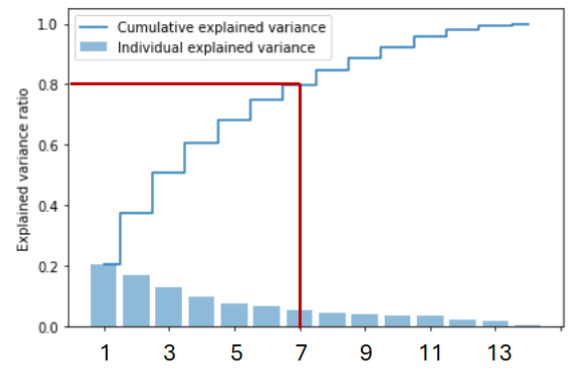
\includegraphics[width=0.4\textwidth]{dr/pca/cev_visualized.png}
\end{figure}


\subsubsection{How to interpret PCs}
The PC's weights can be used to interpret the meaning of the PCs itself: by loking at them we can 
have a clue about which dimensions go along in the same direction, and from them we can give to the PC some kind of interpetation
\begin{figure}[h]
    \centering
    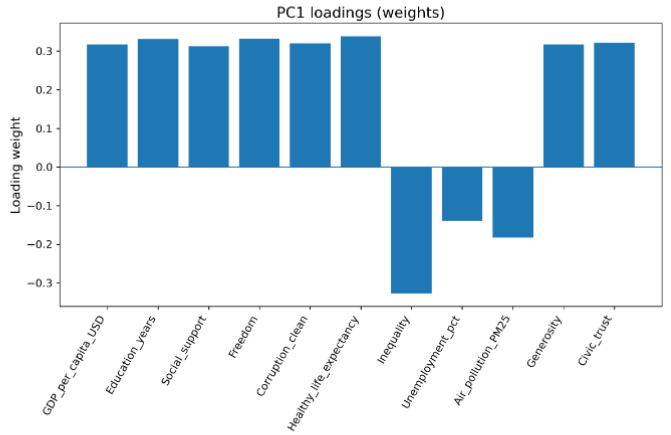
\includegraphics[width=0.4\textwidth]{dr/pca/interpret_pcs.png}
\end{figure}
\hfill\\

Another useful tool to interpret the PCs' meaning is the \textbf{biplot}: using
PCs as axis, we plot both the points projected on the PCA dimensions and the original
features.
\begin{figure}[h]
    \centering
    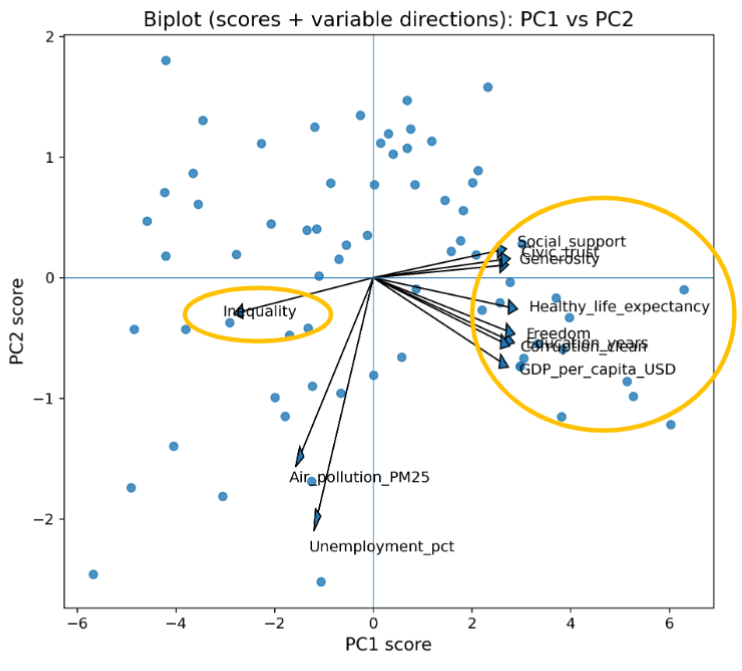
\includegraphics[width=0.4\textwidth]{dr/pca/biplot_example.png}
\end{figure} \hfill \\
and we interpret the meaning as following:
\begin{itemize}
    \item \textbf{arrow direction}: along which direction the feature increases
    \item \textbf{arrow length}: how strongly the features is represented by
    these PCs
    \item \textbf{angle between arrows}: relationship between original features
\end{itemize}



\subsection{Non-Linear dimensionality reduction}
In real-life data usually we can assume the \textbf{Manifolds assumption}:
\begin{center}
    \textit{High-dimensional real data is not scattered uniformly across the ambient 
    space (i.e., the space spanned by the d-original dimensions). Rather, it often 
    lies on (or near to) a much lower dimensional CURVED manifold.}    
\end{center}
\begin{figure}[h]
    \centering
    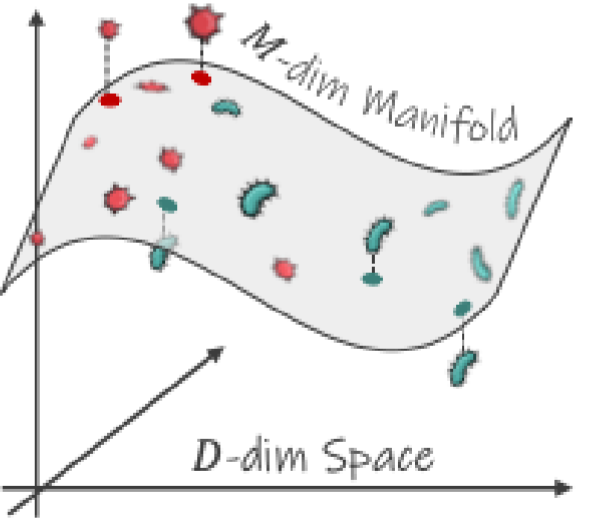
\includegraphics[width=0.2\textwidth]{dr/non_linear/manifold_vis.png}
\end{figure}
PCa is a linear DR techinque, but for real data we need techniques able to properly
model complex non-linear shapes.

%-----------------------------------------------------------------------------------------
\subsubsection{Kernel PCA methods}
This family of methods follows the idea that \textit{data might be non-linear in $\real
^D$ but might become "more linear" after a non-linear feature mapping $\phi(\cdot)$}.
The non-linear transformation is called \textbf{bias expansion} $\phi: \real^p \rightarrow 
\real^q$ and can be choosen accordingly to the analyst's assumption about the shape of the feature; 
usually we take $q>p$ and transform the sampled data into an higher-dimensional space.\\
\hfill \\

We define the basis-expanded matrix $\Phi=(\phi(x_1)\dots \phi(x_n))^T\rightarrow
\Sigma=\Phi^T\Phi$.\\ However, for highly-dimensional projections this approach could
be computationally expensive. In those cases we can take advantage of the
\textbf{kernel trick}: we can compute $\Sigma_{i,j}=k(x_i,x_j)$ using a \textit{kernel 
function $k(\cdot)$}, which measures the similarity between two projections and it's 
defined by $k(x_i,x_j)=\langle\phi(x_i),\phi(x_j)\rangle$ \textcolor{gray}{(scalar product)}.\\
\hfill \\

One of the advantages of this method is the ability of untangling circles.
\begin{figure}[h]
    \centering
    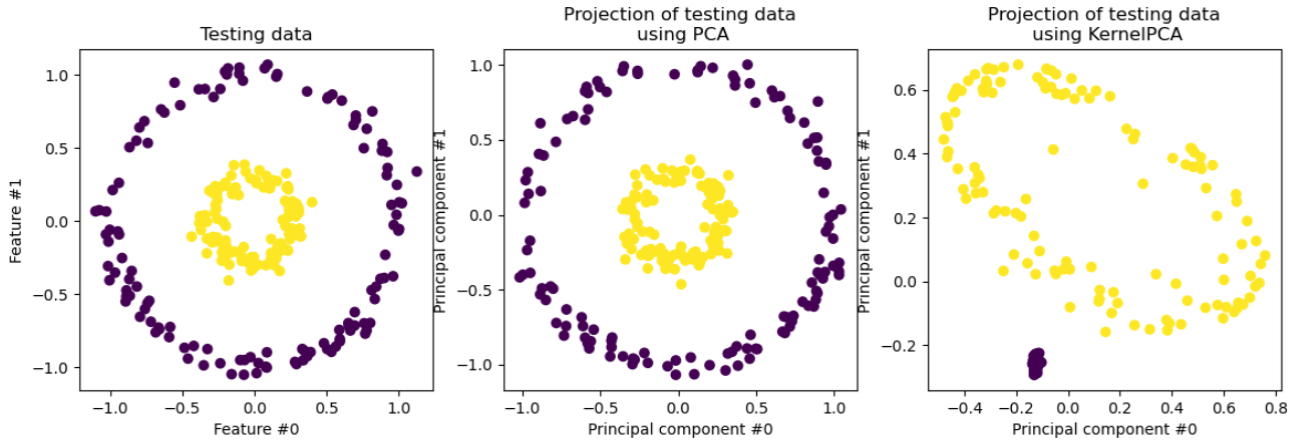
\includegraphics[width=0.8\textwidth]{dr/non_linear/nldr_untangling_circles.png}
\end{figure}
\vspace{0.8cm}

The problem with Kernel PCA is the original space reconstruction: with \textit{linear
PCA} the inverse is explicit and it's exact if projection and original space have the
same dimension, approximante if the projection space has less dimensions than the 
original one.\\
In \textit{Kernel PCA} however $\phi$ is learned/induced by the data
and this could end up in having complex inverse transformations, if not even
non-invertible $\phi$s. Sometimes the only solution to have some reverse-mapping is to rely on
learning the pre-image of the transformation, or more commonly an approximation of it.

\begin{figure}[h]
    \begin{subfigure}{0.48\textwidth}
        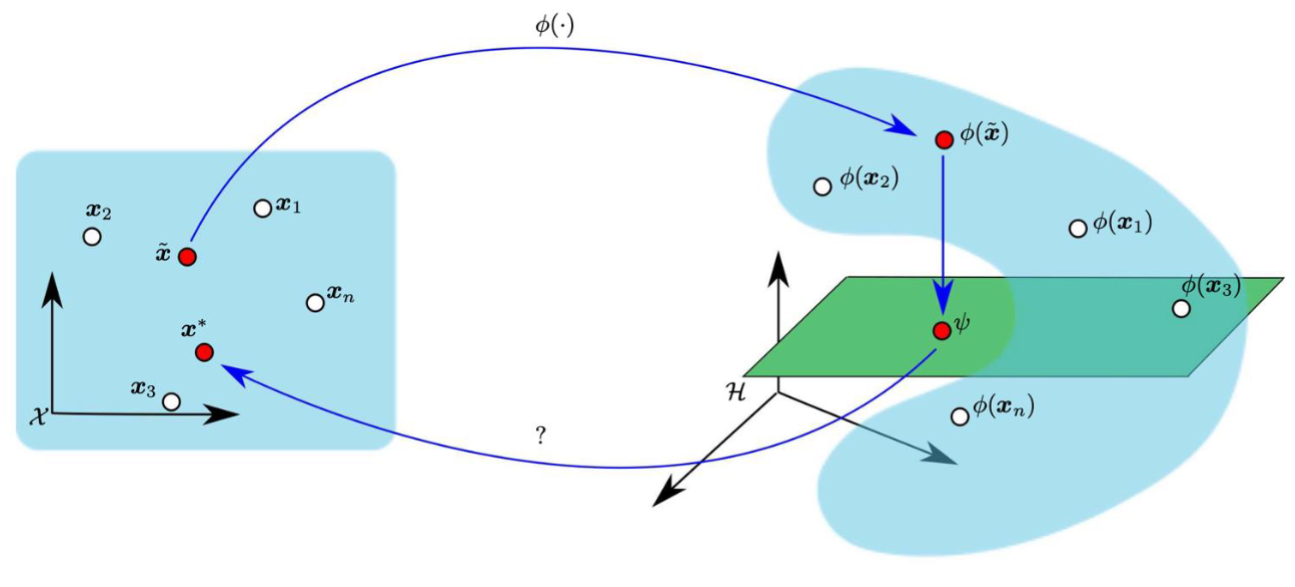
\includegraphics[width=0.95\linewidth]{dr/non_linear/inv_kernelPCA.png}
        \caption*{The idea of non-linear kernel PCA mapping.}            
    \end{subfigure}
    \begin{subfigure}{0.5\textwidth}
        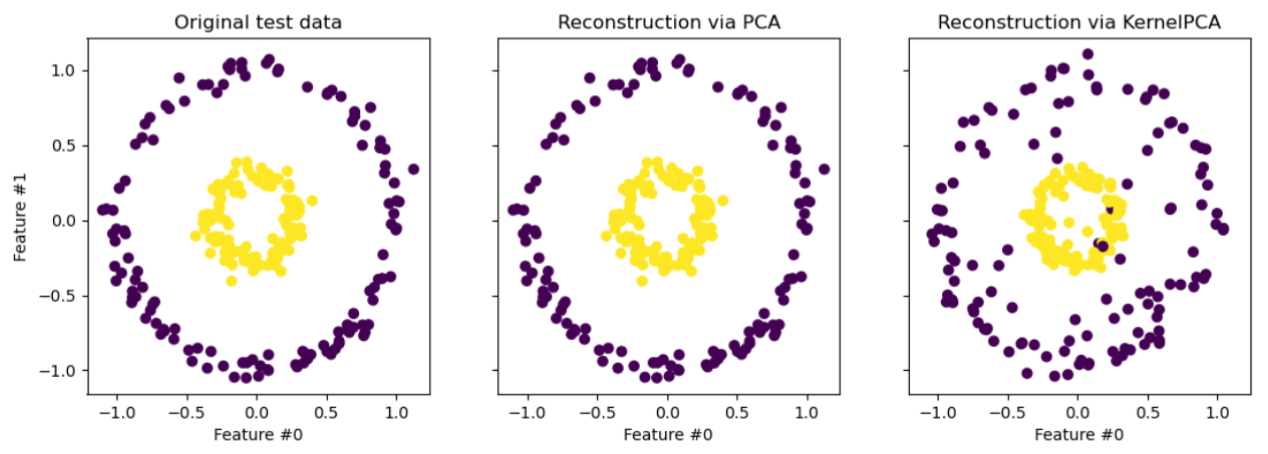
\includegraphics[width=0.95\linewidth]{dr/non_linear/kernel_reconst.png}
        \caption*{Example of non-biective kernel PCA, with loss in the original feature 
        reconstrucion.}    
    \end{subfigure}
\end{figure}
\newpage
\hfill\\
%-----------------------------------------------------------------------------------------
\vspace{0.5cm}
\subsubsection{t-distributed Stochastic Neighbour Embedding (t-SNE)}
The key idea of this family of methods is to \textit{preserve the data geometry by
focusing on local neighbours (points near to each other should remain close to each other after
the projection)}.
\begin{figure}[h]
    \centering
    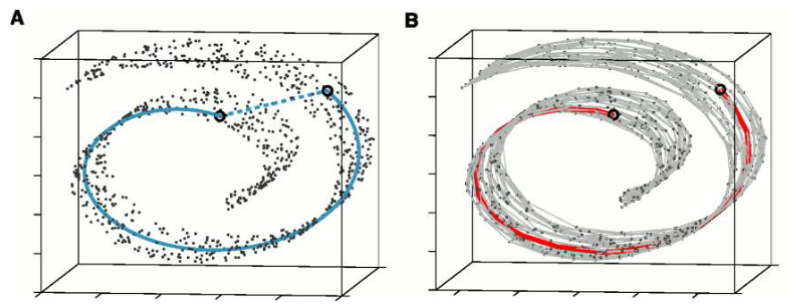
\includegraphics[width=0.6\textwidth]{dr/non_linear/global_vs_local_neigbhbours.png}
    \caption{On the left the distance computed accordingly to global distance; on the
    right the distance is computed using local neighbour.}
    \label{fig:exlocdist}
\end{figure}\hfill \\
Note: This type of methods are really useful for data visualization.\\
\hfill \\

As shown in the Fig \ref{fig:exlocdist} the problem with global similarity is that doesn't
strictly follows the data shape, while based on similarity between point we \dots
watch the recording. 

To do that, we don't need to preserve the distances with respect
to allo the points, but just with his neighbours. This allow to preserve the 
geometric relationship of the data. 
\begin{figure}[h]
    \centering
    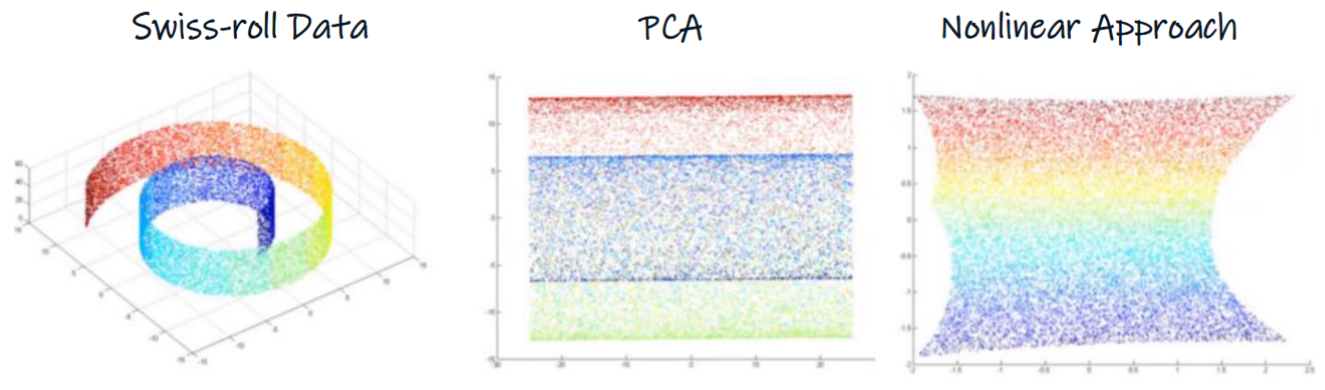
\includegraphics[width=0.6\textwidth]{dr/non_linear/nlpca_shape_preservation.png}
\end{figure}
\hfill \\

t-SNE is mainly focused on preserving neighbourhood: points that are close in the
original space should stay clore in the mapping, otherwise they aren't forced to 
preserve the "right far distance" (not blobal distance as focus).
\hfill \\
I translate the distance into probability: if two points are close, they have higher
probability of being neighbours.
To determine the neighbourhood concept, the t-SNE firstly determines the \textbf{
similarity score} between points based on the distance between them and a \textit{
probability distribution}, which allows to decrease the probability smoothly base 
on the distance between points
\begin{figure}[h]
    \centering
    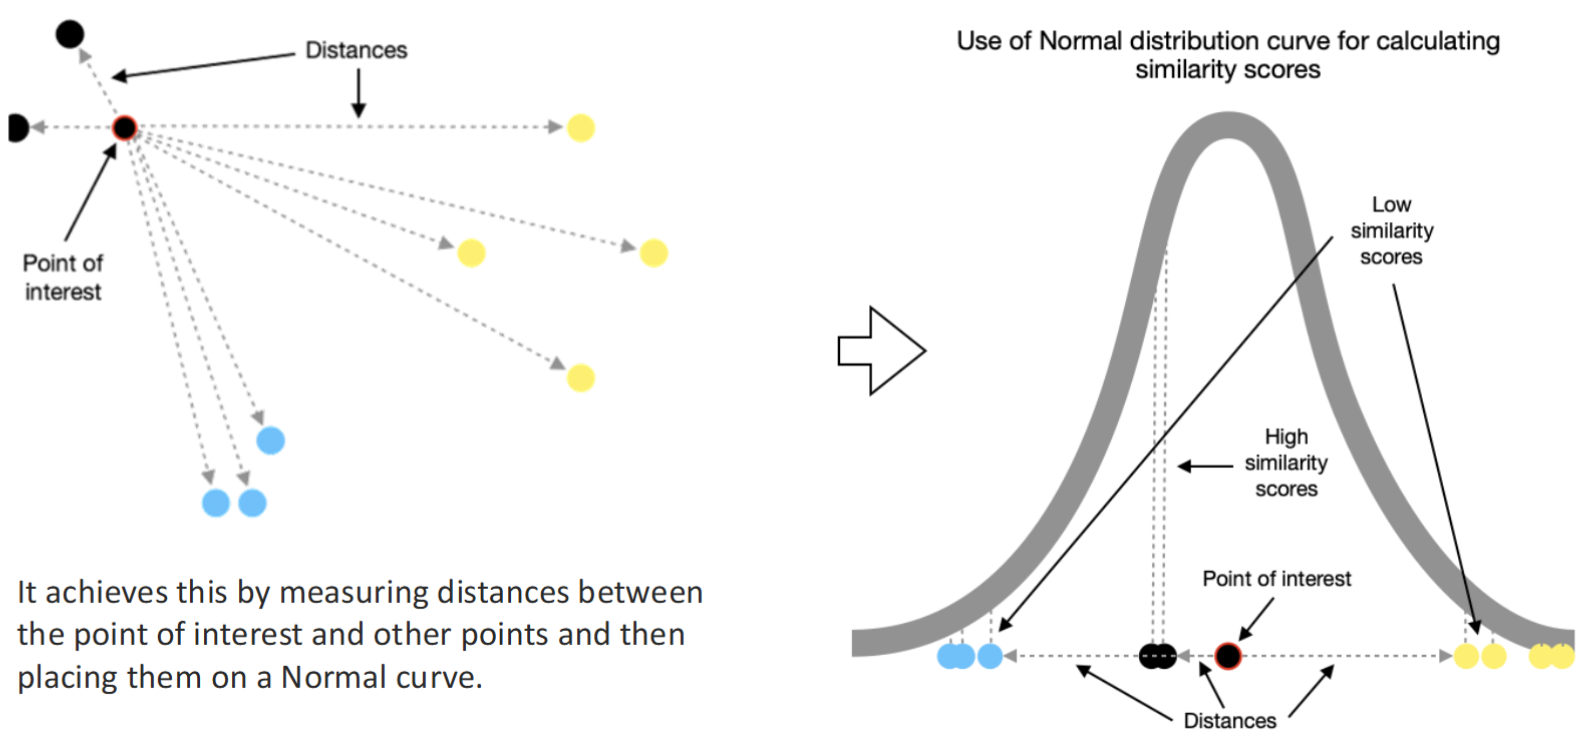
\includegraphics[width=0.55\textwidth]{dr/non_linear/tSNE-similarity.png}
\end{figure}

For each pair of points $i,j$ we could define the \textbf{Gaussian neighbourhood 
distribution} (fore example) as \textcolor{gray}{(we could think about is as "the 
probability that $x_i$ would pick $x_j$ as neighbour")}:
\begin{equation}
    p_{j|i}= \begin{cases}
        \cfrac{exp(-\| x_i - x_j \|^2/(2\sigma_i)^2)}{\sum_{j\neq i}exp(-\| x_i - x_j 
        \|^2/(2\sigma_i)^2)} & j\neq i \\
        0 & j=i
    \end{cases}
\end{equation}
then to make the relationship symmetric $p_{ij} = \frac{p_{i|j}+p_{j|i}}{2}$.\\
To project as much as possible these similarities on a low-dimensional spaces, instead
of using normal distribution t-SNE use \textit{t-student} to discern due its heavier
tails

For the low-dimensional space we use instead a \textit{t-student distribution}: by 
projecting the data on fewer dimensions, the points will end up being more squashed 
together, making the Normal distribution not suited (it will end up considering all the 
points in the same cluster). The \textit{t-student} instead having heavier tails make
the probability distribution more evenly spread, leveraging the dimensionality reduction
squash effect (also called \textit{crowding problem}) $\rightarrow$ thanks to the heavier
tails, low-D points can be pushed away without making $q_{ij}$ too small.
\begin{equation}
    q_{ij}= \begin{cases}
        \cfrac{(1-\| y_i - y_j \|^2)^{-1}}{\sum_{j\neq i}(1-\| y_i - y_j \|^2)^{-1}} 
        & j\neq i \\
        0 & j=i
    \end{cases}
\end{equation} 
\hfill \\

Using different distributions and different dimensionality, we end up with two different
\textbf{similarity matricies}, and out objective becomes making them look alike as much 
as possible $\rightarrow$ minimizingthe mismatch between $p_{ij}$ and $q_{ij}$. To do
tath we iterate to end up with a low-D similarity matrix that is similar to the original
one.
\begin{figure}[h]
    \centering
    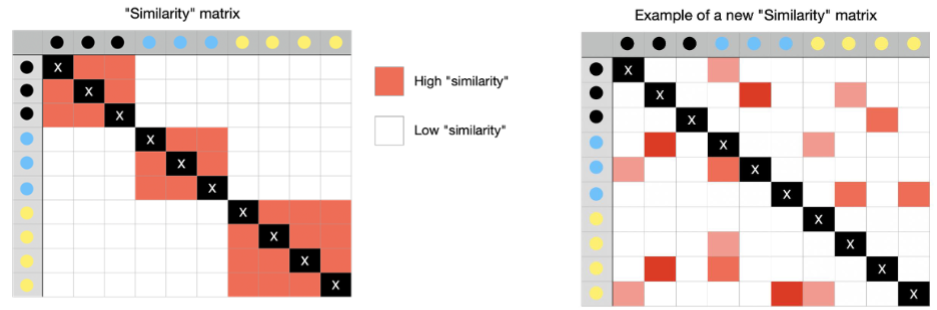
\includegraphics[width=0.6\textwidth]{dr/non_linear/similmat_comparison.png}
\end{figure}
\begin{equation}
    C(Y) = KL(P | Q) = \sum_{i\ne j} p_{ij}\log \frac{p_{ij}}{q_{ij}}    
\end{equation}
the difference is computed using \textit{KL divergence}, which is a way to measure distance
between probabilities.
\\
This cost heavily penalizes high mistatch and has strong local structure preservation 
\textcolor{gray}{(focus on maintainig true neighbours, not in preserving the true 
far-away distances)} $\rightarrow$ this might cause \textbf{distortion of the global
structure}.
\\
\textbf{Perplexity on hyperparameters}\\
How do we choose hyperparameters? By changing the variance of the distributions we shape
the concept of neighbourhood, changing the preplexity ($perp. ~ \sigma^2$) $\rightarrow$ 
we have to balance between the dimensionality of the data and  how many cluster do we 
expect to have.
\begin{figure}[h]
    \centering
    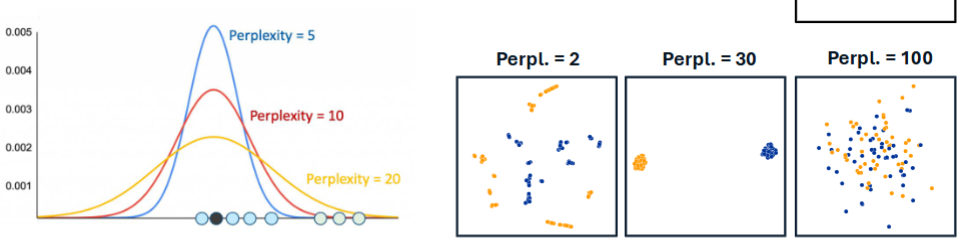
\includegraphics[width=0.6\textwidth]{dr/non_linear/hyperparam_perplexity.png}
\end{figure}

%-----------------------------------------------------------------------------------------
\subsubsection{Uniform Manifold APproximantion (UMAP)}
The idea of this method is still to preserve neighbourhood but using different approach:
we build a graph in the high-D space linking the points and we try to apply the same graph
on the low-D space to preserve the structure as much as possible.
\begin{figure}[h]
    \centering
    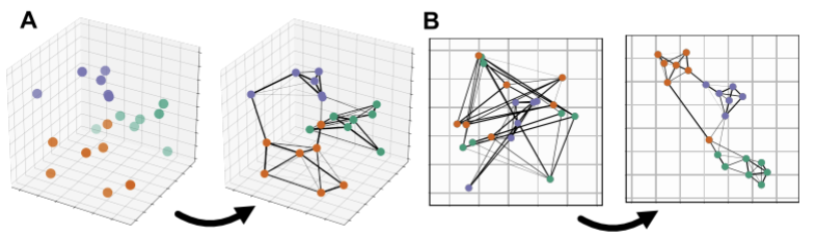
\includegraphics[width=0.5\textwidth]{dr/non_linear/umap_concept.png}
    \caption{High-D and low-D graphs using UMAP}
\end{figure}
To build the graph, we place circles centered on the data points, and those points having
overlapping circles are neighbours $\rightarrow$ the circle's radius is critical
\begin{figure}[h]
    \centering
    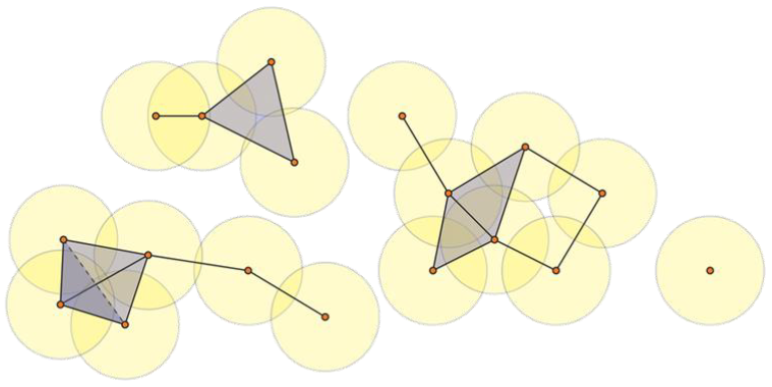
\includegraphics[width=0.4\textwidth]{dr/non_linear/umap_radius.png}
\end{figure}
To overcome this problem we can extend the algorithm using a \textit{local radius}: instead
of fixed value, for some point we use the distance from its n-th neighbour as radius, and
using somethig similar to a distance as weight of the edge.
\\
Differently to \textit{t-SNE} and its perplexity, this method tunes two different parameters:
\begin{description}
    \item[Nearest neighbour]: the number of neighbours used for the high-D radius, tunes how
    "wide" my clusters will be
    \item[Min distance]: tunes how much tightly data points are gonna be projected in the 
    low-D space \textcolor{gray}{(I'm putting some external knwoledge to make the data plots
    more clear, very dangerous for inference)}.
\end{description}
\hfill \\
UMAP algorithm is way faster that t-SNE, uses a more efficient to shuffle the data.

%-----------------------------------------------------------------------------------------
\subsubsection{AutoEncoders (AE)}
The problem with \textit{Kernel PCA} is that is really difficult to turn back in the
original data space, while \textit{t-SNE/UMAP} are good for visualization but we can't
do inference with them. The idea is to use a new class fo algorithms capable of going
back and forth between high-D and low-D spaces: \textit{Autoencoders}, composed by two
subfunctions, \textit{encoders} and \textit{decoders}, which learn a non-linear mapping 
between spaces.
\begin{description}
    \item[Encoder (compression)]: \hfill \\
    $z_i=f_\theta(x_i),\ f_\theta:\real^D\rightarrow\real^d$ with $z=f_\theta(x)=\sigma(Wx+b) 
    \rightarrow$ the conders apply a non-linear function \ssigma := activation function on 
    pre-linear-combination $Wx+b$ (\ssigma, $W$, $b$ are parameters)
    \item[Decoders (reconstruction)]: \hfill \\
    $\hat{x}_i=g_\phi(z_1),\ g_\phi:\real^d\rightarrow \real^D$ with $\hat{x}=g_\phi(z)=
    \rho(Vz+c)$; the structure is the same as encoder, just in the other way around (and 
    uses \diff params).
\end{description}
\begin{figure}[h]
    \centering
    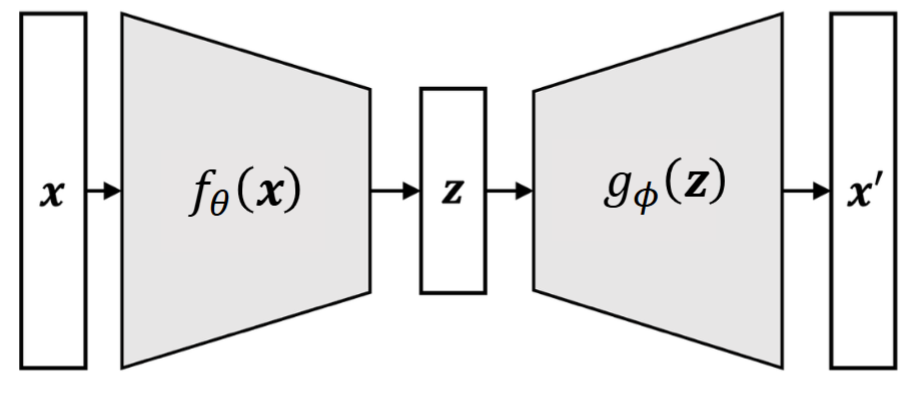
\includegraphics[width=0.35\textwidth]{dr/non_linear/autoencoders__sketch.png}
\end{figure}
We can tune the parameters to lose as less information as possible during compression/
reconstruction phase, maybe even remove only the information we want to loose $\rightarrow$
Autoencoders allow us to decide what we lose.\\
\vspace{0.5cm}

\textbf{Training objective}: to tune the parameter sets $\theta,\phi$ in order to make the
reconstruction as losless as possible, we have to \textit{train the algoirthm}:
\begin{equation}
    \hat{x}_i=g_\phi(f_\theta(x_i)) \rightarrow \min_{\theta,\Phi} \frac{1}{n} 
    \mathcal{L}(x_i,\hat{x_i})
\end{equation}
Commonly we choose $\mathcal{L}(x_i,\hat{x}_i)=\| x_i-\hat{x}_i \|_2^2$.

\hfill\\
\textcolor{gray}{
This method doesn't allow to explain the data variabilty induced by each dimension like in 
PCA, however stiil allow to tune the level the information/varibaility we want to keep
$\rightarrow$ very useful to identify data anomaly: if a point is very far away the original
space will be projected far away, and also during the reconstrucion phase the decoder will try
to reconstruct it as normal point, giving high reconstruction error and displaying on which 
dimension the anomalies are. 
}

\subsubsection{How to choose non-linear DR methods}
Based on your goal:
\begin{itemize}
    \item \textbf{Data visualization}: use \textit{UMAP} as default, good balance between 
    execution time and accuracy (sometimes preserves also the global organization); use 
    \textit{t-SNE} when your main concern is displaying local cluster separation.
    \item \textbf{Nonlinear feature engineering (reusable mapping)}: \textit{autoencoders}
    are the best to find explicit mapping; \textit{Kernel PCA} is a good fit for medium-sized
    dataset for which we have some domain model.
    \item \textbf{Data interpretability (like PCA loadings)}: PCA, that's it    
\end{itemize} 
\vspace{0.3cm}
Method recomendations:
\begin{description}
    \item[Kernel PCA]\hfill
        \begin{description}
            \item[\textcolor{green}{Pros}]: linearize non-linear structure if a kernel can and
            the dataset sie is manageable.
            \item[\textcolor{red}{Cons}]: not suited for large datasets, and urge the need for
            inverse function, usually only computable trough pre-image approximation. 
        \end{description}
    \item[t-SNE/UMAP]\hfill   
        \begin{description}
            \item[\textcolor{green}{Pros}]: use them for visual exploration of local clusters.
            \item[\textcolor{red}{Cons}]: due the global structure distrortion, they can't be
            used to draw conclusions and doing inference.
        \end{description}
    \item[AutoEncoders]\hfill
        \begin{description}
            \item[\textcolor{green}{Pros}]: learn mapping between spaces, allowing reconstruction
            or interpretability capabilities.
            \item[\textcolor{red}{Cons}]: complexity overhead, with smaller datasets there might
            be overfitting.
        \end{description}   
\end{description}
\section{Clustering}
This class is a type fo \textit{unsupervised learning} in which we assume that the 
data has some kind of unkwon structure, and we wan to figure it out. To do that we
try to accomplish two things: 
\begin{itemize}
    \item minimize distance between datapoints of the same cluster
    \item maximize distance between \diff clusters
\end{itemize}
\begin{figure}[h]
    \centering
    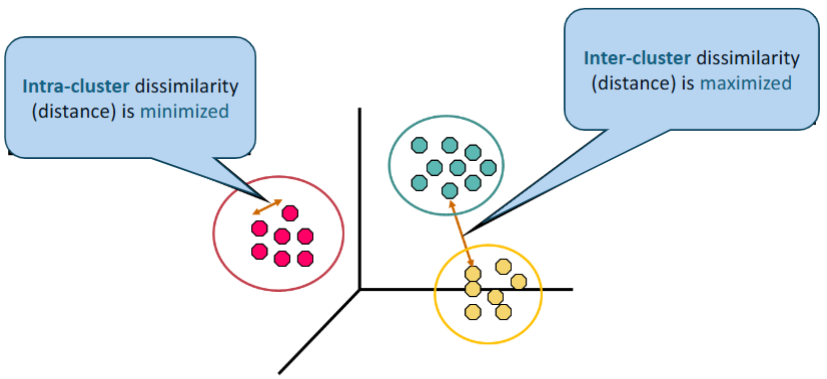
\includegraphics[width=0.3\textwidth]{clustering/cluster_example.png}    
\end{figure}
The clustering output is really subjective and depend what we're trying to achieve
and our conception of \textbf{similarity}. We have to define two elements:
\begin{description}
    \item[Distance metric]: tells what makes two object similar/dissimilar
    \item[Clustering algorithm]: procedure to compute groups/clusters
\end{description}
\vspace{0.5cm}

%-----------------------------------------------------------------------------------------
\subsubsection*{Distance metrics}
The definition of Distance Metrics depends mostly on the type of the data features.
Some common ones are:
\begin{itemize}
    \item \textbf{Euclidean distance}: $d_E(x,q)=\sqrt{\sum_{i=1}^n(x_1-q_1)^2}$

    \item \textbf{Squared Euclidean Distance}: $d_{E^2}(x,q)=(d_E(x,q))^2 
    \rightarrow$ with respect to $d_E$ it gives more emphasys to outliners 
    \textcolor{gray}{(distance is squared)}

    \item \textbf{Standardize Euclidean Distance}: $d_{SE}(x,q)=\sqrt{\frac{1}
    {s_i^2}(x_i-q_i)} \rightarrow$ weights each dimension by something inverse
    to its variability, favouring those dimensions that doens't change too much

    \item \textbf{Chebychev Distance}: $d_ {\max}(x,q)=\max_i|x_i-q_i|$ 
    \textcolor{gray}{(just the max, not really useful)}

    \item \textbf{Manhattan Distance}: $d_M(x,q)=\sum_{i=1}^n|x_i-q_i| \rightarrow$
    gives the \# step to reach a destination in a grid by moving up and down, lot of
    usage in many fields

    \item \textbf{Correlation-based Distance}: $d_R(x,q)=1-\cfrac{s_{x,q}}{\sqrt{s_x}
    \sqrt{s_q}}=1-\cfrac{\sum_i(x_i-\bar{x})(q_i-\bar{q})}{\sqrt{\sum_i(x_i-\bar{x})
    ^2\sum_i(q_i-\bar{q})^2}} \rightarrow$ this measures allow to get an idea about
    the distance between feature trends distance 
\end{itemize}
\hfill \\
Highly suggested to use $d_R$ in the project\\
\hfill \\
To compare the datapoint features, we must be sure that everyone is using the same
measurement unit.

\newpage
%-----------------------------------------------------------------------------------------
\subsubsection*{Clustering algorithms}
There are several way to categorize these methods:
\begin{description}
    \item[Hard clustering]: each datapoint can be only in one cluster
    \item[Soft clustering]: each datapont might be in more clusters at the same time
\end{description}
\begin{figure}[h]
    \centering
    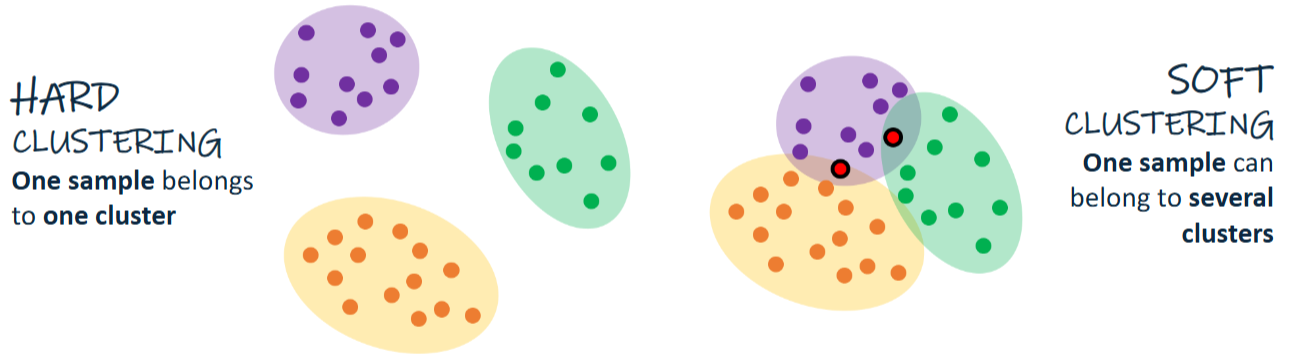
\includegraphics[width=0.6\textwidth]{clustering/soft_vs_hard_clustering.png}
\end{figure}

\begin{description}
    \item[Flat clustering]: all clusters are at the same level
    \item[Hierachical clustering]: the cluster are under some hierarchy (dendogram)
\end{description}

% this is just a summary, place it at the begging of the relative section
\begin{comment}
Partition-based clustering: A partitioning method creates k partitions from given set of n data objects.
Initially, each data objects are assigned to some of the partitions. An iterative relocation technique is used to
improve the partitioning by moving objects from one group to another. E.g. k-means, k-median;

Hierarchical clustering: hierarchical clustering is a method of cluster analysis that seeks to build a hierarchy of
clusters. E.g. Agglomerative, Divisive;

• Density-based clustering: identify distinctive clusters in the data, based on the idea that a cluster/group in a
data space is a contiguous region of high point density, separated from other clusters by sparse regions. e.g.
DBSCAN;
is more similar ~

• Probabilistic clustering: models the data as generated by a mixture of probability distributions. Each
cluster is a component (e.g., a Gaussian) and each observation has a membership probability (soft
assignment)
not hard assignment, more flexibility 
\end{comment}

\vspace{0.5cm}
%-----------------------------------------------------------------------------------------
\subsection{K-means algorithm}
In this algorithm we priorly fix the number of clusters $k$, starting from an initial 
assignment and itereatively moving datapoints between the clusters.

% maybe make it like code snippet
\begin{enumerate}
    \item define $k \rightarrow C_1\dots C_k$ clusters
    \item randomly assign each point to some cluster $C_i$ and compute the centroid for 
    that set of points
    \item re-assign each point to the closest centroid cluster, ending up possibly with 
    new point in each cluster
    \item recompute the centroids, and iterate from \textit{step 2}
\end{enumerate} 
We iterate unitl the algorithm converges, e.g. the points won't change cluster.

\begin{figure}[h]
    \centering
    % --- First row ---
    \begin{subfigure}[t]{0.3\textwidth}
        \centering
        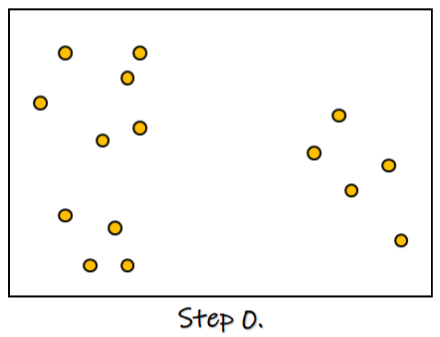
\includegraphics[width=\linewidth]{clustering/kmeans/kmean_step0.png}
    \end{subfigure}
    \hspace{0.3cm}
    \begin{subfigure}[t]{0.3\textwidth}
        \centering
        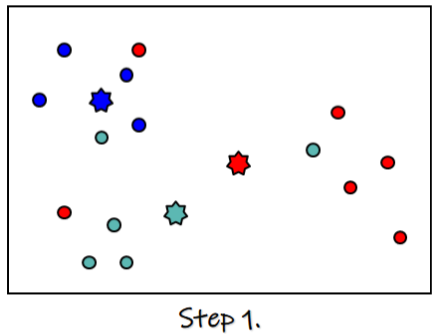
\includegraphics[width=\linewidth]{clustering/kmeans/kmean_step1.png}
    \end{subfigure}
    \hfill \\
    % --- Second row ---
    \begin{subfigure}[t]{0.3\textwidth}
        \centering
        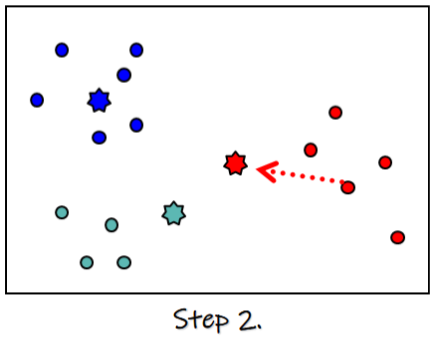
\includegraphics[width=\linewidth]{clustering/kmeans/kmean_step2.png}
    \end{subfigure}
    \hspace{0.3cm}
    \begin{subfigure}[t]{0.3\textwidth}
        \centering
        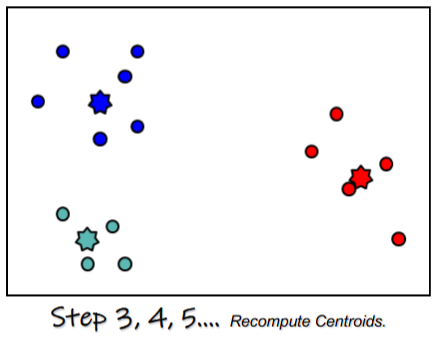
\includegraphics[width=\linewidth]{clustering/kmeans/kmean_step3.png}
    \end{subfigure}
\end{figure}

\newpage
\textbf{Limitations} of this algorithm:
\begin{itemize}
    \item the algorithm output strongly depends on the initial random assignment; if 
    there is some structure probably the algorithm will converge at the same result, but 
    if this structure is not so evident the outcome might be very sensitive.\newline
    \begin{figure}[h]
        \centering
        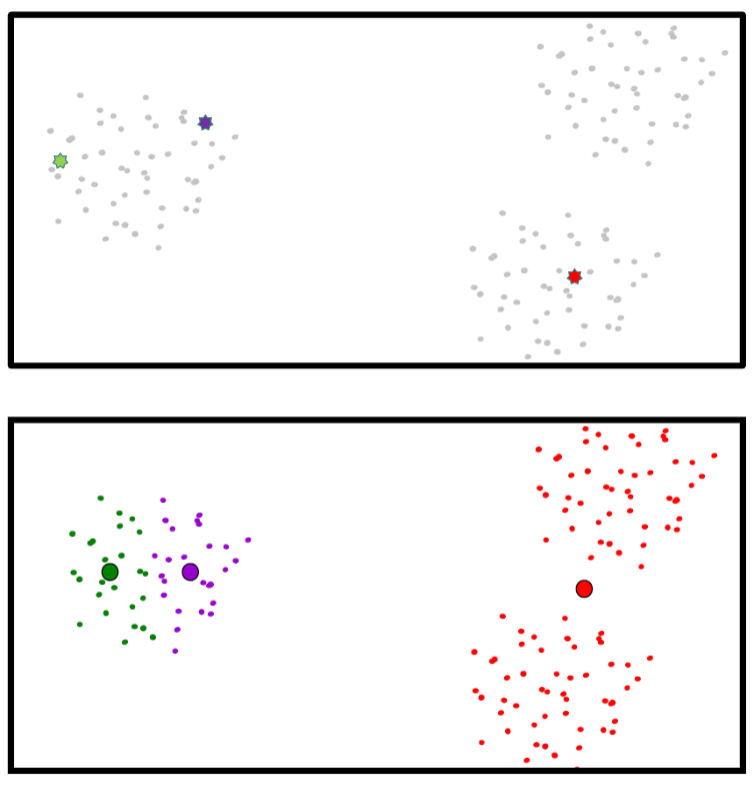
\includegraphics[width=0.2\textwidth]{clustering/kmeans/init_assignment_error.png}
    \end{figure}
    To reduce this influence we could try out multiple seeds in parallel and choose at the 
    end the best result.

    \item we have to choose $k$ in advance, maybe without clear idea of we're doing
    
    \item the distance used affects a lot the centroid: if we use \textit{Euclidean 
    Distance} our computation is going to be very sensitive to outliers
    \begin{figure}[h]
        \centering
        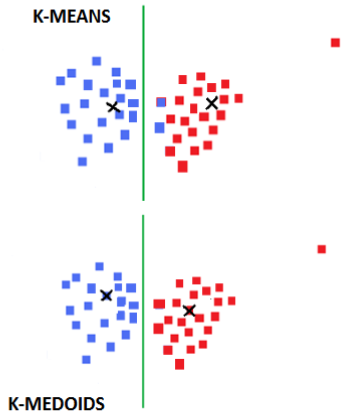
\includegraphics[width=0.2\textwidth]{clustering/kmeans/k_medoids.png}
    \end{figure}
    We can resolve this by choosing another method to compute distances: instead of using 
    $d_E$ we use the \textbf{mode}, which are more robuts to utliers $\rightarrow$ the 
    \textit{medoid} is also more reasonable to use since we'll end up with something that 
    is a real point of the cluster \textcolor{gray}{(like the most representative point)}.
    
    \item with strange-shape clusters, K-means makes a very bad work (how can we know that 
    in advance? You can't) $\rightarrow$ k-means fits well spherical/hellipsoidal 
    datashapes
\end{itemize}

%-----------------------------------------------------------------------------------------
\subsection{Hierarchical clustering}
%It can be used for many many things, not only for clustering
This method builds a hierarchy among the clusters using a \textbf{Distance Matrix D}, which 
contains the distance between each pair of samples. To stop the procedure we have to define 
a \textbf{cutting criterion} to stop the construction of the \textbf{dendogram} := 
representation of your cluster.
\begin{figure}[h]
    \centering
    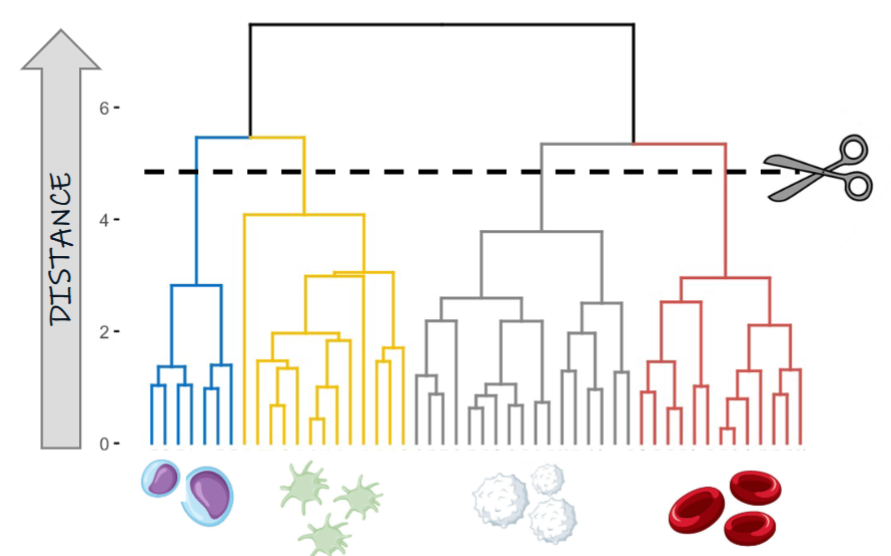
\includegraphics[width=0.5\textwidth]{clustering/hierachical/dendogram_example.png}
\end{figure}
The algorith can both start by considering each datapoint in a \diff cluster and then
merging them, or start from a one big cluster and progressively split it.

\begin{enumerate}
    \item start from considering each datapoints as a cluster per se
    \item merge the two closer clusters and take a "center" (linkage methods)
    \item recompute the set of points and iterate starting from 1
\end{enumerate}
By merging the cluster $D$ become smaller at each iteration.

By using this algorithm we can also highligh noisy datapoints and anomalies: if a point is 
added very late in the cluster, maybe it's just an anomaly $\rightarrow$ this method can
also be used for anomaly detection.

\paragraph{Linkage methods}\hfill\\
How do we computer the "center" between build-up clusters? 
\begin{description}
    \item[Single link]: cluster-distance is based on the two closest points from each 
    cluster
    \begin{figure}[h]
        \centering
        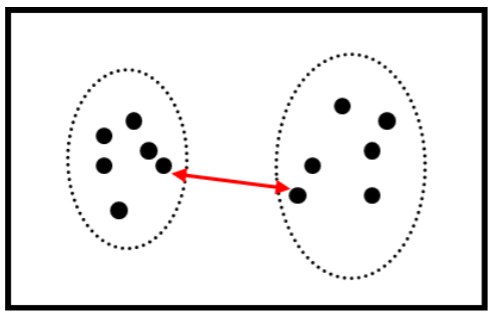
\includegraphics[width=0.2\textwidth]{clustering/hierachical/single_linkage.png}        
    \end{figure}

    \item[Average link]: cluster-distance is based on the average position of the cluster
    datapoints
    \begin{figure}[h]
        \centering
        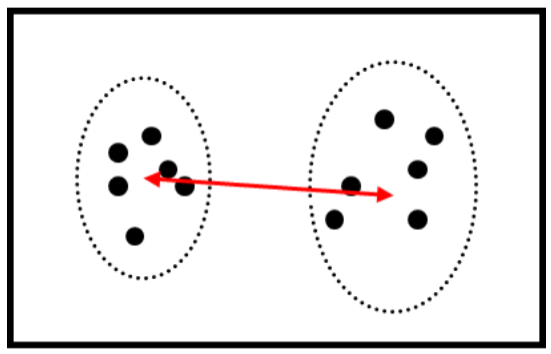
\includegraphics[width=0.2\textwidth]{clustering/hierachical/avg_linkage.png}        
    \end{figure}

    \item[Complete link]: cluster-distance is based on the most distant points from each
    cluster
    \begin{figure}[h]
        \centering
        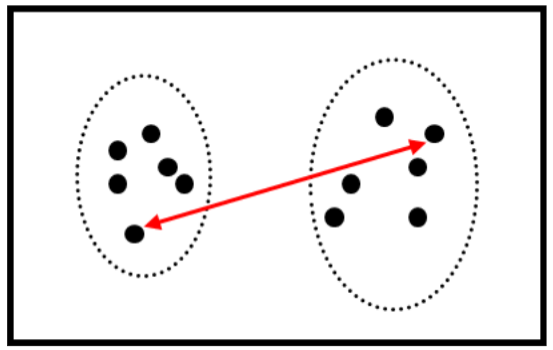
\includegraphics[width=0.2\textwidth]{clustering/hierachical/complete_linkage.png}        
    \end{figure}

\end{description}
There is no rule of thumb, start with the average and adjust things.
% what about the mode for this one?

%-----------------------------------------------------------------------------------------
\subsection{Evaluating cluster quality}
How do we eavulate if our clusters make sense if we don't have an output reference?

\subsubsection{Within Cluster Sum of Square (WCSS)}
WCSS measures the variability of the observations within each cluster.
\begin{equation}
    WCSS = \sum_i\sum_{p\in C_i} dist(p,C_i)^2
\end{equation}

The smaller our clusters are, the lower(better) the value of WSS. However by following
this metric, we get that the best result is we each datapoint form a cluster per-se. So we 
don't want to minimize this, otherwise is useless; we need just to find a point in which it
doesn't decreases a too much.\\
\hfill \\
With this method we're also looking at how similar points within the same cluster are, 
without considering the other goal of clustering: distance between \diff clusters.

\paragraph{Solhouette Score}
This metrics takes into account both the distance between points in the same cluster and
the distance from other cluster's points.

\begin{enumerate}
    \item $\forall$ point $i$ get all the distances from the points within the same
    cluster $a(i)$
    \item $\forall$ point $i$ get the distance from the points in the nearer cluster $b(i)$
    \item $\forall$ point $i$ get the average of both $\bar{a}(i),\bar{b}(i)$
    \item get the \textbf{Silhouette score} $\forall\ i$: $sil(i)=\cfrac{\bar{b}(i)-\bar{
    a}(i)}{\max\{\bar{a}(i),\bar{b}(i)\}}$
    \item get the \textbf{Silhouette score for cluster $k$}: $sil(C_k)=\frac{1}{|C_k|}\sum_{ 
    i\in C_k}sil(i)$
    \item get the \textbf{Silhouette score for overhall clustering}: $sil(C)=\cfrac{1}{K}
    \sum_{k=1}^K sil(C_k)$
\end{enumerate}
\begingroup
\let\clearpage\relax
\section{Simple linear regression}
Now we switch focus on \textit{supervised learning}: that is, deriving/predicting the value of some feature given the values of others.
Taking this example on \textcolor{green}{exam score vs study hours}, what if we'd like to predict the score
of the next person who studies 5 hours per week?
\begin{figure}[h]
    \centering
    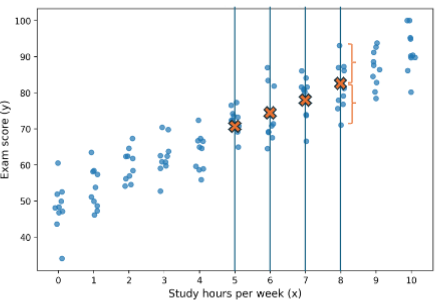
\includegraphics[width=0.3\textwidth]{linearmodel/lm_example.png}
\end{figure}

Obviously we take as predcitor the mean of the score samples for that amount of studying hours; we can do the same for the other sets of points. We can see there is a linear model between the 
study hours and the mean of the exam scores: $\mathbb{E}[\text{score}|\text{study\ hours}] = f(\text{study\ hours})$.
\vspace{0.2cm}

So we want to create a model to shape this relation:
\begin{description}
    \item[] $X$ := independent/predictor variable (usually known)
    \item[] $Y$ := dependent/response variable \arrow it's a random variable (due \seps)
    \item[] \seps := random deviation/error \arrow it's a random variable
\end{description}
\begin{equation*}
    \mathbb{E}[Y|X]=\beta_0+\beta_1X+\varepsilon
\end{equation*}
where $\beta_0,\beta_1,\sigma^2$ are parameters and we \textbf{assume} that $\mathbb{\varepsilon}=0$
,$\mathbb{V[\varepsilon]}=\sigma^2$ and that's symmetrically distributed.\\ 
\vspace{0.2cm}
Interpretation of the parameters:
\begin{itemize}
    \item \textbf{intercept} $\beta_0$: "height"/base-line of the model, where the line intercepts the 0
    \item \textbf{slope} $\beta_1$: how much my model increases for unit increment of the 
    predictor $x$ \textcolor{gray}{(by studying 1 hour more, I will improve my score by $beta_1$)}
    \item $\sigma^2$: how much our response is spread along the model prediction
\end{itemize}
\begin{figure}[h]
    \centering
    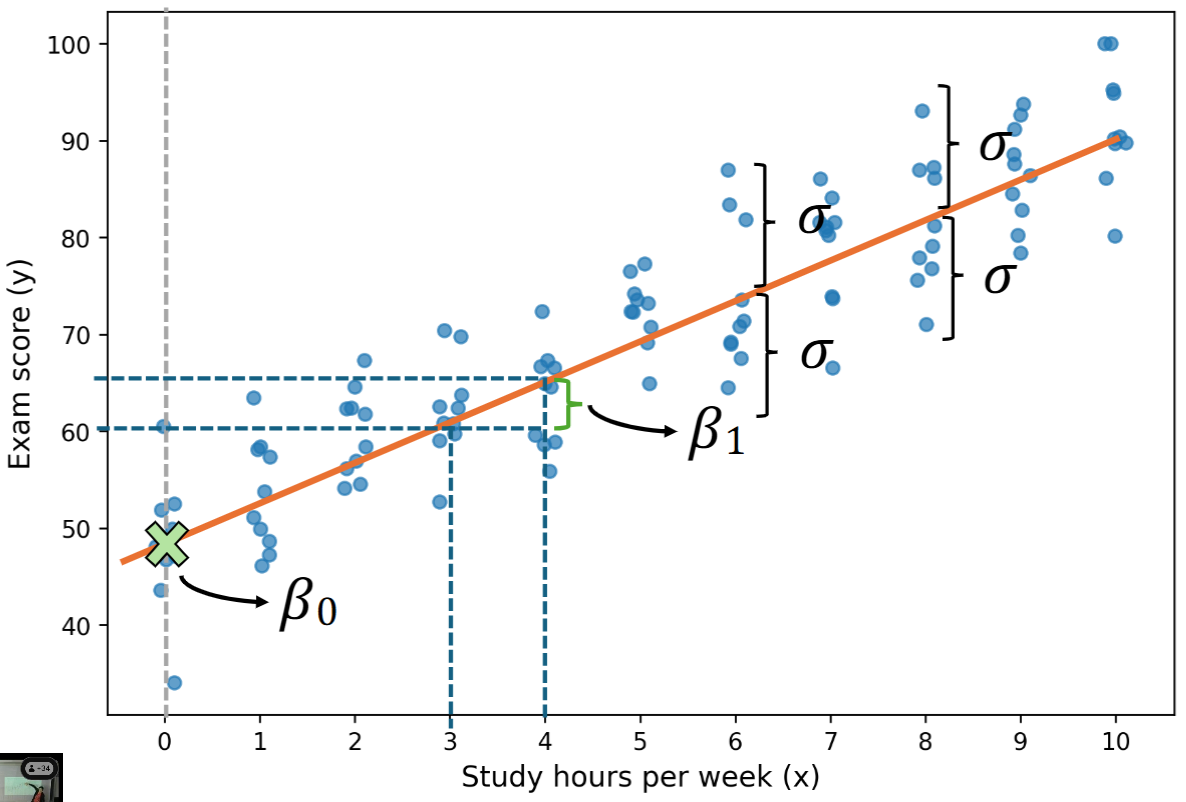
\includegraphics[width=0.4\textwidth]{linearmodel/lm_param_interpretation.png}
\end{figure}
\newpage
Let's start with the following assumptions on the errors: we assume that the spread of our model on each predictor value is the same (\textit{homoscedasticity}) and that $\varepsilon \sim \mathcal{N}(0,\sigma^2)$.
\begin{figure}[h]
    \centering
    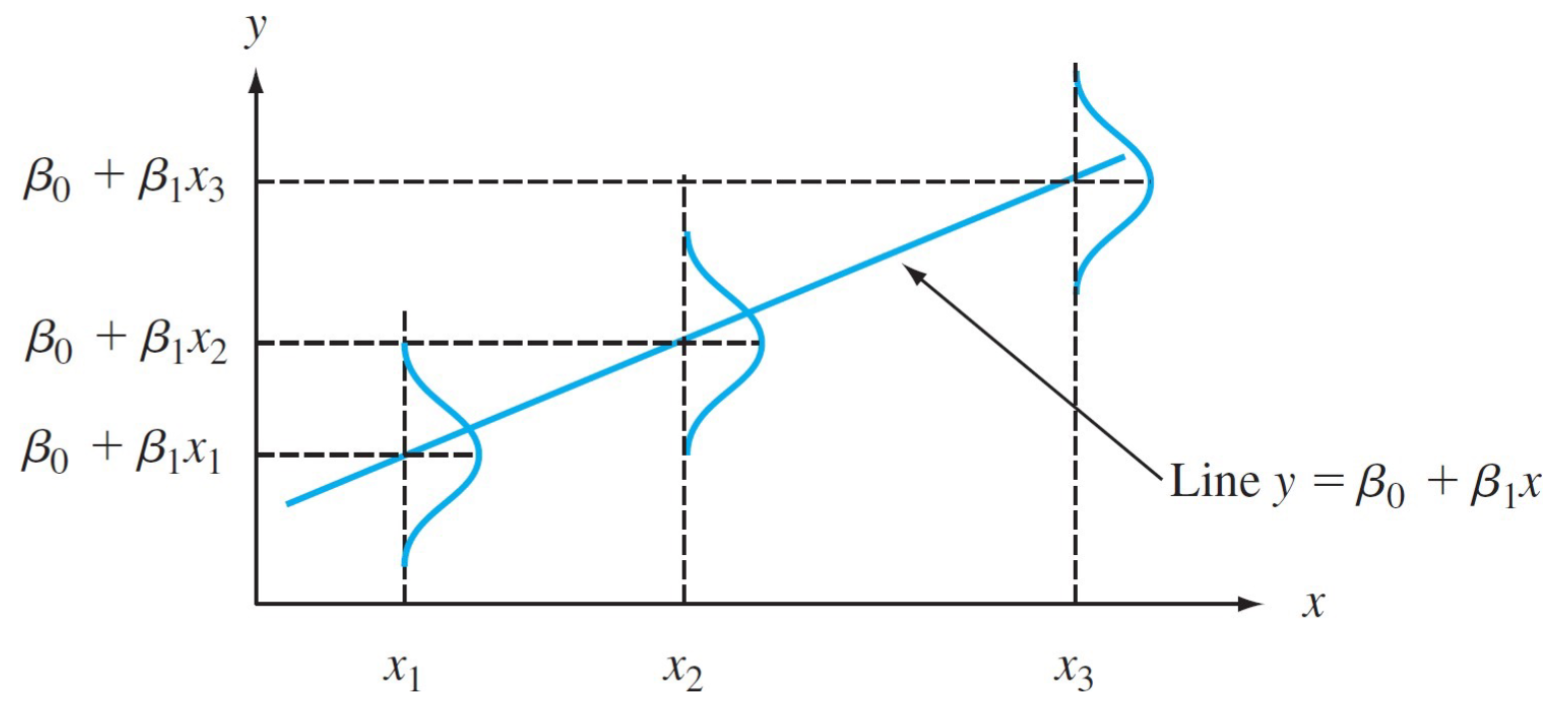
\includegraphics[width=0.4\textwidth]{linearmodel/err_assumption.png}
\end{figure}

\subsection{Model estimation}
The model parameters are not usually known, so how do we estimate them from a set of samples $(x_1,y_1
\dots (x_n,y_n))$?\\
We assume $y_i = \beta_0 +\beta_1 x_i +\varepsilon_i,\ \ \varepsilon_i\sim\mathcal{N}(0,\sigma^2)
\rightarrow y_i\ |\ x_i\sim\mathcal{N}(\beta_0+\beta_1 x_i, \sigma^2)$ and we are going to select those parameters that minimize the squared error:
\begin{equation*}
    \hat{\beta}_0,\hat{\beta}_1 = \arg\min_{\beta}\sum_i\varepsilon_i^2=\sum_i\left(y_i-(\beta_0+
    \beta_1 x_i)^2\right)
\end{equation*}
\begin{figure}[h]
    \centering
    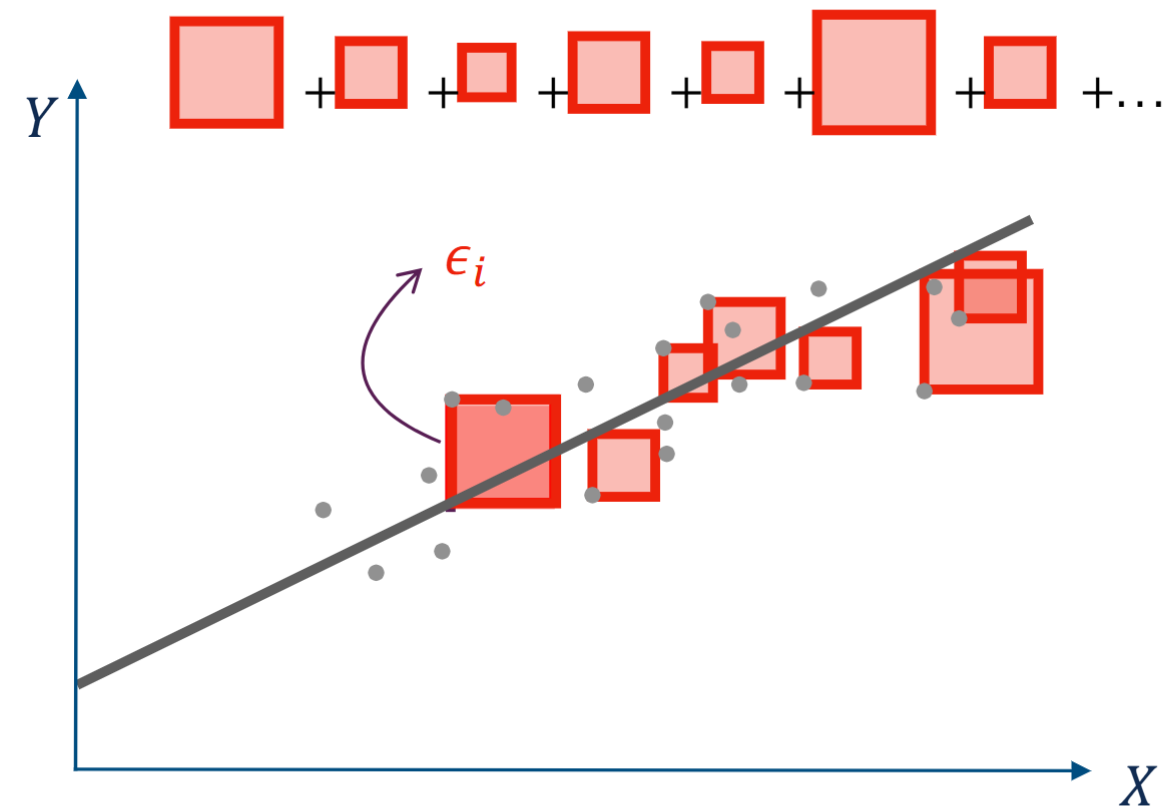
\includegraphics[width=0.4\textwidth]{linearmodel/square_error_visualized.png}
\end{figure}


\textcolor{gray}{(you can skip the computation of the closed formula)}
$$
\begin{cases}
    \frac{\partial}{\partial \beta_0} \sum_{i} (y_i - [\beta_0 + \beta_1 x_i])^2 = -2 \sum_{i} (y_i - \beta_0 - \beta_1 x_i) = 0 \\
    \frac{\partial}{\partial \beta_1} \sum_{i} (y_i - [\beta_0 + \beta_1 x_i])^2 = -2 \sum_{i} x_i (y_i - \beta_0 - \beta_1 x_i) = 0
\end{cases} \implies
$$ $$
\begin{cases}
    \sum_{i} y_i = n\beta_0 + \beta_1 \sum_{i} x_i \\
    \sum_{i} y_i x_i - \beta_0 \sum_{i} x_i - \beta_1 \sum_{i} x_i^2 = 0
\end{cases} \implies
$$ $$
\begin{cases}
\bar{y} = \beta_0 + \beta_1 \bar{x} \\
\sum_{i} x_i^2 \beta_1 = \sum_{i} y_i x_i - (\bar{y} - \beta_1 \bar{x}) \sum_{i} x_i
\end{cases} \implies
$$ $$
\begin{cases}
    \bar{y} = \beta_0 + \beta_1 \bar{x} \\
    \beta_1 \left( \sum_{i} x_i^2 - \frac{(\sum_{i} x_i)^2}{n} \right) = \sum_{i} x_i y_i - \frac{\sum_{i} x_i \sum_{i} y_i}{n}
\end{cases} \implies
$$ $$
\begin{cases}
    \hat{\beta}_0 = \bar{y} - \hat{\beta}_1 \bar{x} \\
\hat{\beta}_1 = \cfrac{\sum_{i=1}^n (x_i - \bar{x})(y_i - \bar{y})}{\sum_{i=1}^n (x_i - \bar{x})^2}
\end{cases}
$$

Even if it might look like PCA, now we're not minimizing the distance of the line from the point
\textcolor{gray}{(is not even a distance, is not orthogonal)} but we're just computing the error 
between the model and the actual data. 

\subsection{Model assessment}
\textbf{After estimating our model, we'd like to check its goodness}.\\
To do so, first we compute the variance of out estimations $\hat{\beta}_0,\hat{\beta}_1$ and then we use it to build a \textbf{confidence interval CI}.

$$
\begin{cases}
Var(\hat{\beta}_0) = \sigma^2 \left[ \frac{1}{n} + \cfrac{\bar{x}^2}{\sum_{i=1}^n (x_i - \bar{x})^2} \right] \\
Var(\hat{\beta}_1) = \cfrac{\sigma^2}{\sum_{i=1}^n (x_i - \bar{x})^2}
\end{cases} \implies
\begin{cases}
\hat{\beta}_0 \sim \mathcal{N}(\beta_0, Var(\hat{\beta}_0)) \\
\hat{\beta}_1 \sim \mathcal{N}(\beta_1, Var(\hat{\beta}_1))
\end{cases}
$$
with an $\alpha$\% CI $\hat{\beta_i}\pm t_{n-2,1-\alpha/2}\sqrt{Var(\hat{\beta}_i)}$

\vspace{0.2cm}
One critical aspect to check is whether the computed CI contains zero or not: if it does the coefficient might be 0, meaning that $Y$ and $X$ are not really dependent \arrow if the CI is completely above/below zero, even by a small amount, no problem.
\vspace{0.1cm}
\begin{figure}[h]
    \centering
    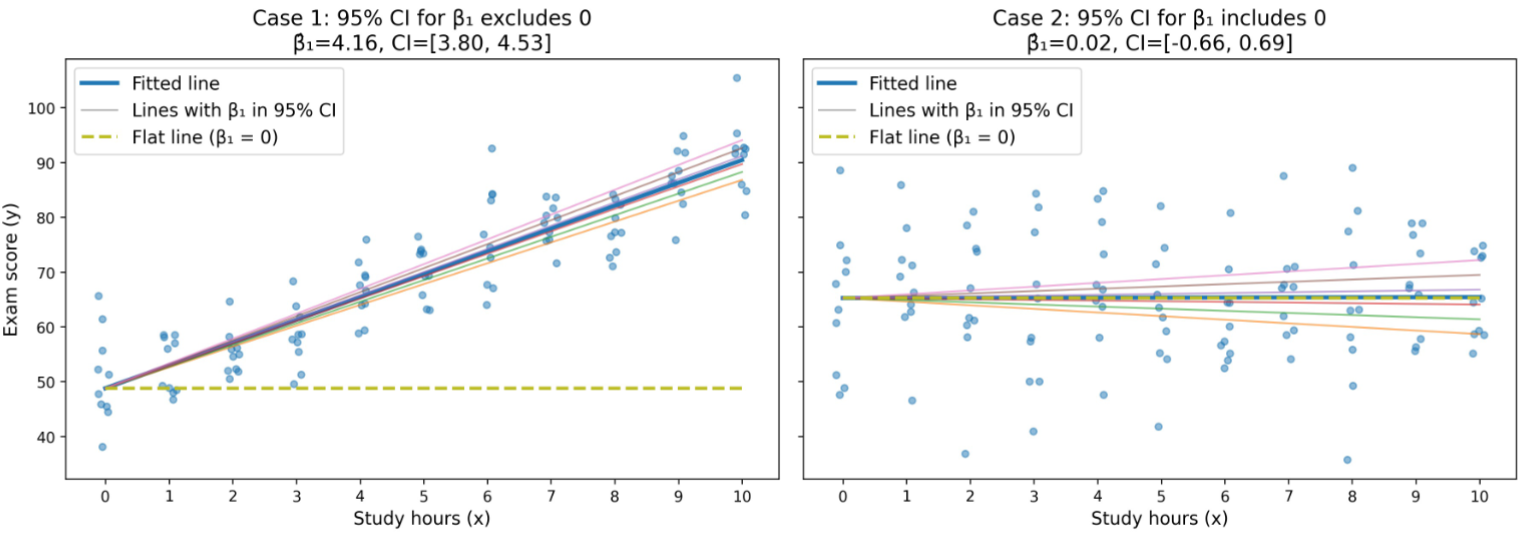
\includegraphics[width=1\linewidth]{linearmodel/lm_param_CI.png}
\end{figure}

\vspace{0.4cm}
We could also approach the problem from another perspective using \textbf{tests}: we'd like to quantify how much we are sure that the estimate won't be zero.
\begin{equation*}
    H_0: \beta_i=0\ \ \text{vs}\ \   H_1: \beta_i\ne0
\end{equation*}

and the statistic used for the test (below) measures the dispersion of the coefficient estimate. If we get small t p-value under the hypo that the coefficient is zero, it means that I'm seeing
something very unlikely\arrow I have evidence that the coefficient is not 0. 
 
\begin{equation*}
    t_i = \cfrac{\hat{\beta_i}}{SE(\hat{\beta_i}) = \sqrt{Var(\hat{\beta_i})}}\sim t_{n-2}
\end{equation*}

\newpage
\subsubsection{Variability explained}
After the parameter estimation, we can compute the \textbf{residuals} $\hat{e}$ := difference 
between our model and the real output.
$$
\begin{aligned}
\hat{y}_i &\to \hat{\beta}_0 + \hat{\beta}_1 x_i + e_i \\
y_i &\to \beta_0 + \beta_1 x_i + \epsilon_i
\end{aligned}
\implies e_i \neq \epsilon_i
$$

\vspace{0.2cm}
\begin{wrapfigure}[14]{l}{0.5\linewidth}
    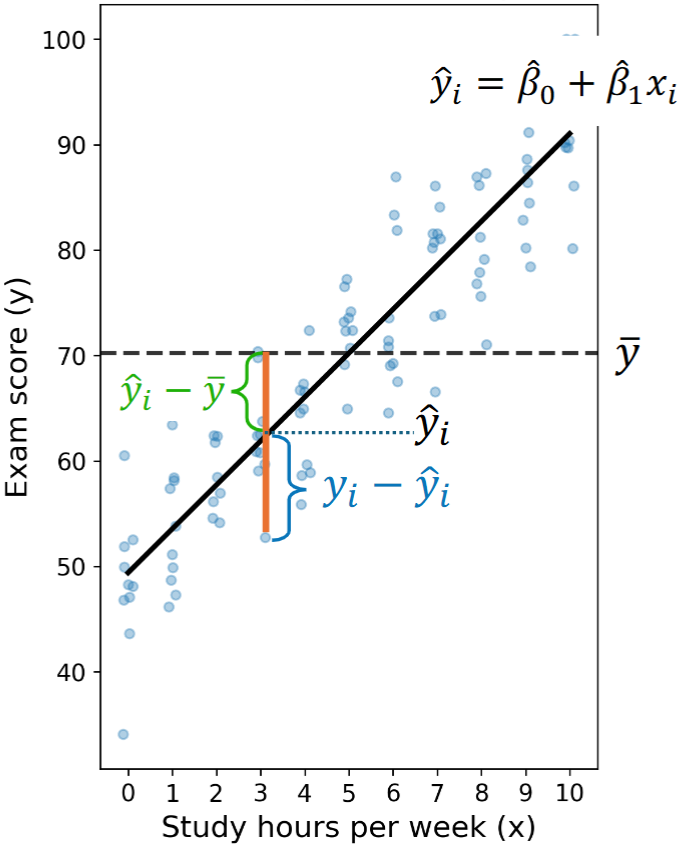
\includegraphics[width=0.4\textwidth]{linearmodel/var_explained.png}
\end{wrapfigure}
If we don't know any model, the only reasonable way to estimate $Y$ is to use $\bar{y}$.
\vspace{0.2cm}
$$
\begin{aligned}
    &\sum_{i=1}^{n} \textcolor{orange}{(y_i - \bar{y})^2} = 
    \sum_{i=1}^{n} \textcolor{green}{(\hat{y}_i - \bar{y})^2} + 
    \sum_{i=1}^{n} \textcolor{blue}{(y_i - \hat{y}_i)^2} \\
    &\begin{matrix}
        \textcolor{orange}{\textbf{TSS}} \\
        \textcolor{orange}{\text{Total Sum of}} \\
        \textcolor{orange}{\text{Squares}}
    \end{matrix} 
    \ =\ 
    \begin{matrix}
        \textcolor{green}{\textbf{ESS}} \\
        \textcolor{green}{\text{Explained Sum}} \\
        \textcolor{green}{\text{of Squares}}
    \end{matrix}
    \ +\ 
    \begin{matrix}
        \textcolor{blue}{\mathbf{RSS}} \\
        \textcolor{blue}{\text{Residual Sum of}} \\
        \textcolor{blue}{\text{Squares}}
    \end{matrix}
\end{aligned}
$$
\vspace{0.3cm}
\begin{description}
    \item[\textcolor{orange}{TSS}]\arrow total variability of the data, is the biggest mistake we
    can make during prediction
    \item[\textcolor{green}{ESS}]\arrow improvement of the model with respect to the simplest predictor ($\bar{y}$), is the amount of data variability captured by our model
    \item[\textcolor{blue}{RSS}]\arrow difference between our model and the real data (error model),
    is the amount of variability we couldn't capture
\end{description}

\vspace{1.8cm}
So to evaluate the goodness of our model we could measure "the \% of variability we capture with our model":
\begin{equation*}
    R^2 = \frac{\textcolor{green}{ESS}}{\textcolor{orange}{TSS}} = 
    1 - \frac{\textcolor{blue}{RSS}}{\textcolor{orange}{TSS}}
\end{equation*}
We can also used an \textit{adjusted version} that penalizes more complex models, making the adoption of a more complex model not always the best option:
\begin{equation*}
    R^2_{adj} = 1-\cfrac{\textcolor{blue}{RRS}/(n-p)}{\textcolor{orange}{TSS}/(n-1)}
\end{equation*}


\subsubsection{Residual variability/prediction error}
We would like to assess a also the variability of our model prediction. To do so, there are several options:
\begin{description}
    \item[Mean Absolute Error (MAE)] 
    plain error average.
    \begin{equation*}
        MAE = \frac{1}{n}\sum_{i=1}^{n}|y_i-\hat{y}_i|
    \end{equation*}
    
    \item[Root mean squared error (RMSE)]
    average prediction error with higher emphasis on large mistakes.    
    \begin{equation*}
        RMSE = \sqrt{\frac{1}{n}RSS}
    \end{equation*}

    \item[Residual Standard Error (RSE)] 
    similar to RMSE, but now we have a penalization for more complex models.
    \begin{equation*}
        \hat{\sigma}^2=\cfrac{RSS}{n-p}
    \end{equation*}
    

\end{description}


\subsubsection{Model usefulness}
Another thing we'd like to evalate is how useful our model is in explaining the relationship between the response and the predictor: our model is useful if $\beta_1\ne 0$, and the more variability is able to caputure the better \arrow we use an \textbf{F-test}.
\begin{equation*}
    H_0:\beta_1 = 0 \rightarrow F=\cfrac{ESS/(p-1)}{RSS/(n-p)}\sim F_{(p-1)(n-p)}
\end{equation*}
Trying to give it an intepretation, if we consider:
\begin{itemize}
    \item $ESS/(p-1)$ as the average explained variability per each parameter
    \item $RSS/(n-p)$ as the average unexplained variability per residual degree of freedom of the data
\end{itemize}
we get that \textit{$F$ compares the "information per parameter" with the "noise per degree of freedom"}.\\
If the statistic is low then there are evidence against the null hypo. Note that in the linear model, the F-test $\equiv$ t-test, giving the same result.


\subsection{Inference on Y}
Our model coefficient are only an estimation of the true system's parameters (the fitted lines has some uncertanty) so instead of point-level prediction we'd like to use intervals to predict our response.

\subsubsection{CI for the mean response}
The problem we're going to answer is in the form "what's the avg exam score of students who studies $x_0$ hours?" \arrow we want to estimate $\mu_{Y|X=x_0}=\mathbb{E}[Y|X=x_0]$ and to do so we use CI.

\begin{equation*}
    \hat{y}_0 \pm t_{n-2,1-\alpha/2}\ \hat{\sigma}\sqrt{\frac{1}{n}+\cfrac{(x_0-\bar{x})^2}
    {\sum_{i=1}^n(x_i-\bar{x})^2}}
\end{equation*}
\begin{figure}[h]
    \centering
    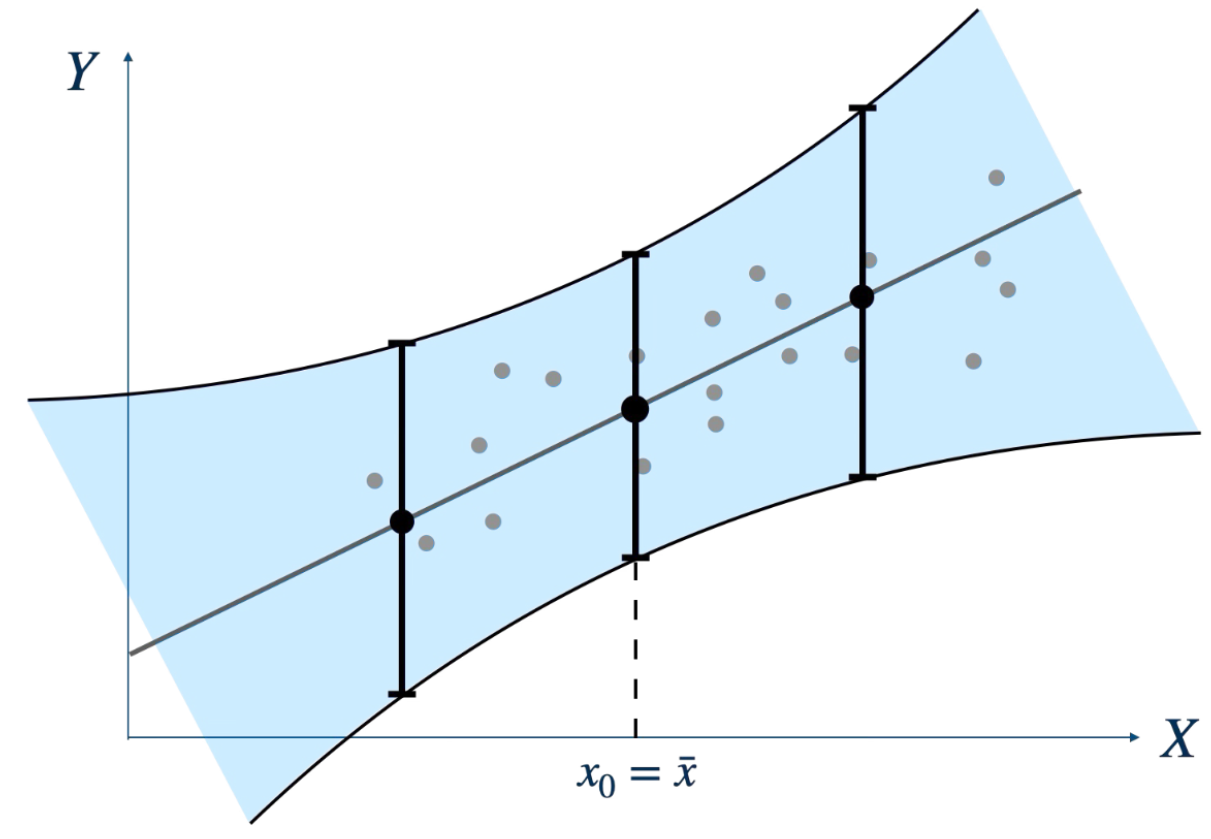
\includegraphics[width=0.4\textwidth]{linearmodel/CI_mean.png}
\end{figure}

We could see that the interval is more narrow near $x_0=\bar{x}$, and makes sense: the further we shift from our dataset center of mass the less density of data, incrementing therefore our uncertanty in those regions.

\subsubsection{Prediction interval}
Now we want to tackle the problem "if the next student studies $x_0$ hours, what range of scores it could hope for?"\arrow we want to estimate $Y_{new}|X=x_0$. In this scenario we have the uncertanty due our model parameters (as before, they're only ans estimation) and due the irreducible noise around the reponse mean \seps.
\begin{equation*}
    \hat{y}_0 \pm t_{n-2,1-\alpha/2}\ \hat{\sigma}\sqrt{1+\frac{1}{n}+\cfrac{(x_0-\bar{x})^2}
    {\sum_{i=1}^n(x_i-\bar{x})^2}}
\end{equation*}


\subsubsection{Comparison: CI vs PI}
\begin{description}
    \item[CIs] show the uncertanty of out model on the population/true system parameter, and the interval becomes larger as the sample's std deviation does (so this issue could be reduced by using a larger sampleset)
    \item[PIs] show the uncertanty on some \textit{specific} value, not on the entire dataset, thus the resulting interval is much wider compared to the CIs
\end{description}

\begin{figure}[h]
    \centering
    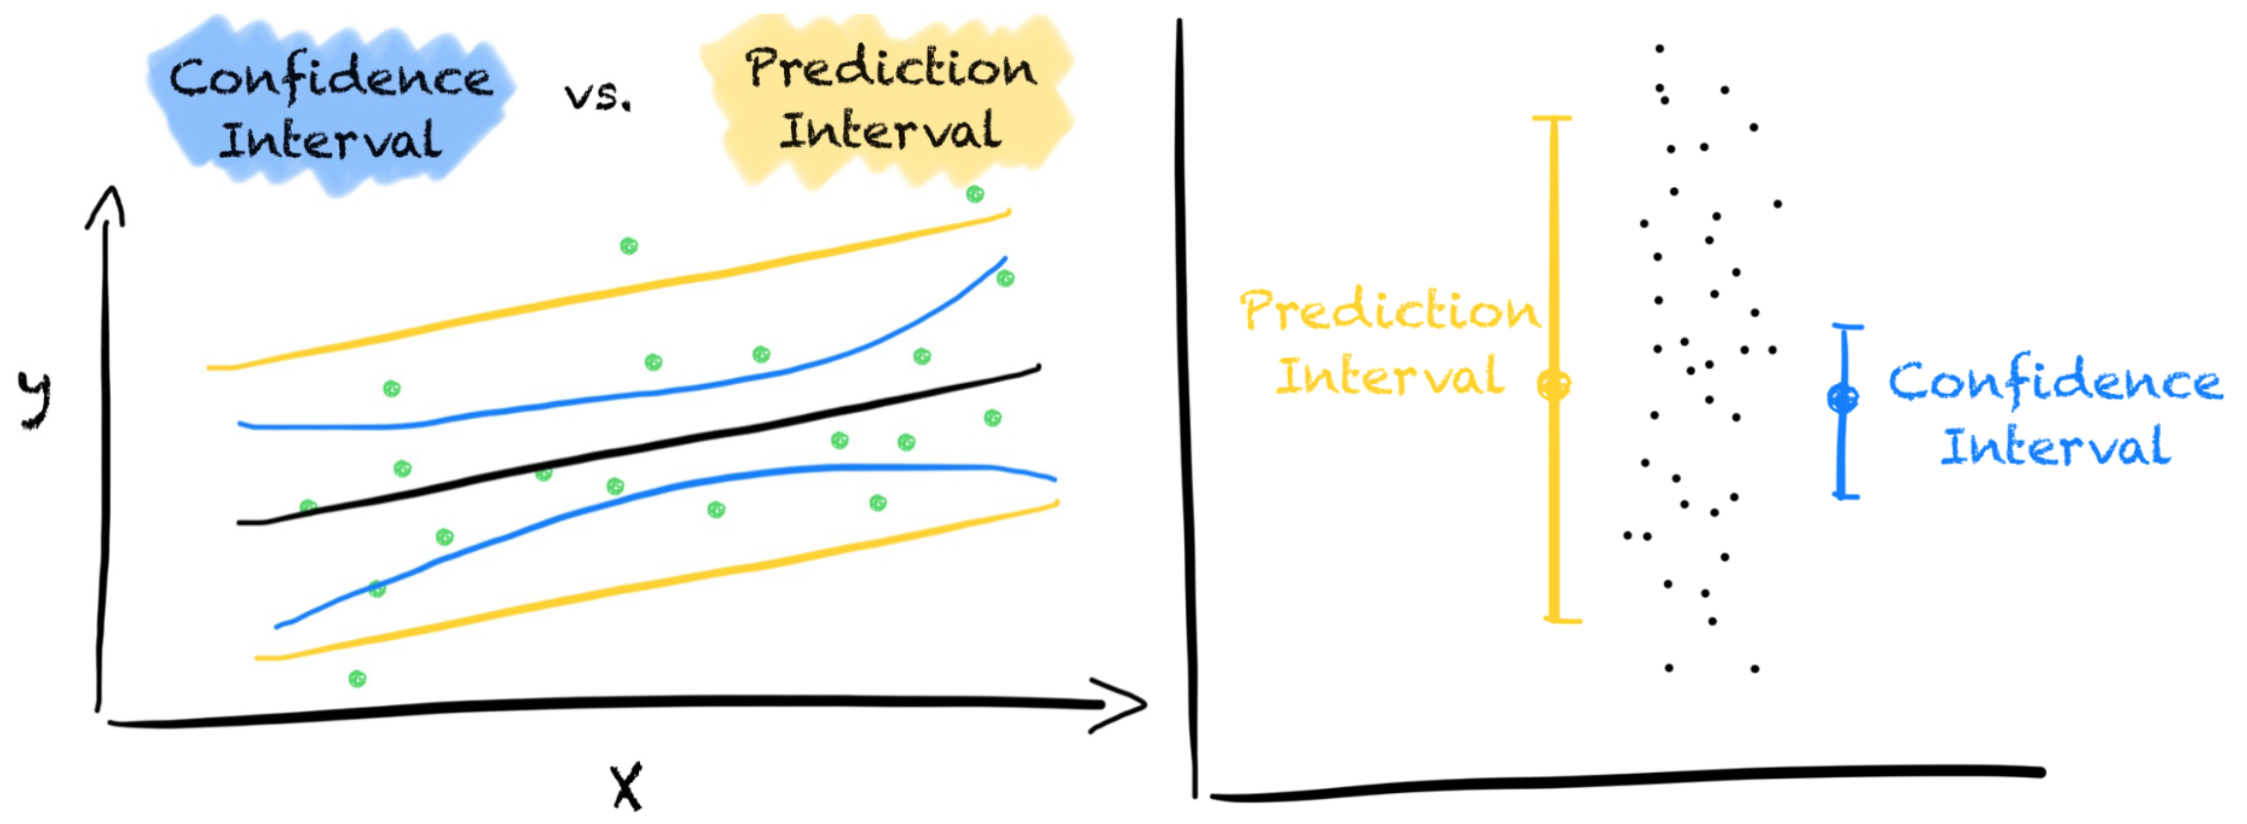
\includegraphics[width=0.75\textwidth]{linearmodel/lm_CI_vs_PI.png}
\end{figure}




\vspace{0.8cm}
\section{Multivalued linear models}
Simple linear regression models could be extended using multiple predictors too: we switch
from a mean response that is a line to something forming a hyperplane in $\mathbb{R}^{p+1}$ (with $p$ predictors): 
\begin{center}
    $\mathbb{E}[Y|X_1=x_1,X_2=x_2]=\beta_0+\beta_1x_1+\beta_2x_2$.    
\end{center}
\begin{figure}[h]
    \centering
    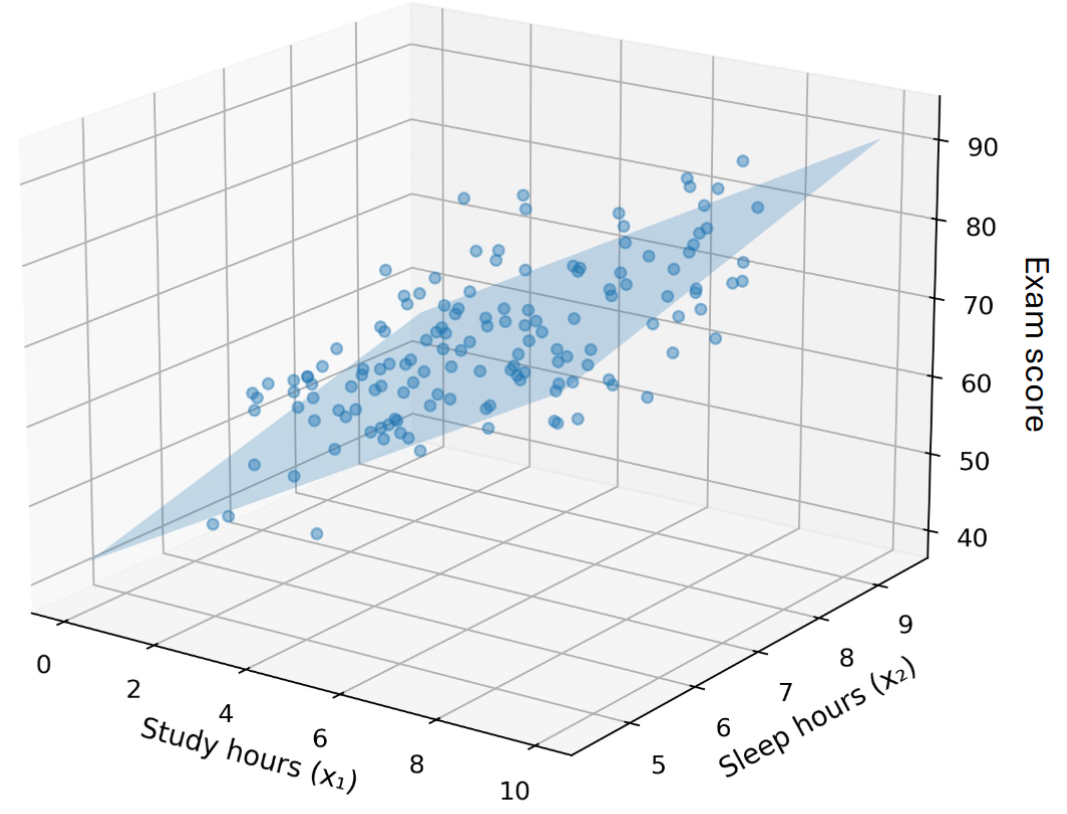
\includegraphics[width=0.4\textwidth]{linearmodel/mlm/mlm_example.png}
\end{figure}\hfill\\

Trying to give an intepretation to the parameters in this new scenario, we have that
\begin{itemize}
    \item $\beta_1$ is the change in mean of $Y$ for the unitary increment of $X_1$, keeping $X_2$
    fixed
    \item $\beta_2$ is the change in mean of $Y$ for the unitary increment of $X_2$, keeping $X_1$
    fixed    
\end{itemize}
So each parameter can stil be interpreted as a slope, but slopes of a plane viewed from \diff angles. This interpretation is conditioned by the other paramters, not marginal.
\newpage
\begin{figure}[h]
    \centering
    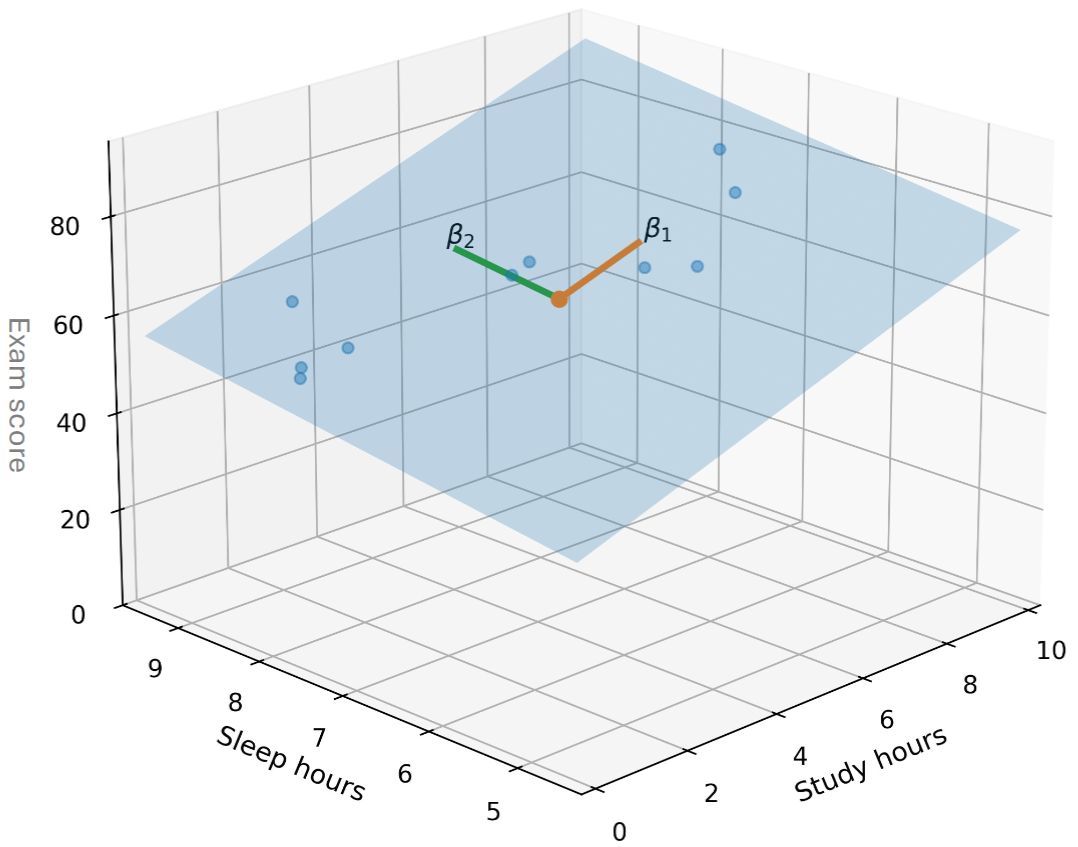
\includegraphics[width=0.4\textwidth]{linearmodel/mlm/mlm_slope_intepret.png}
\end{figure}

So in general we have predictors $x_i\in\real^p$, responses $y_i\in\real$ and noise \seps under the assumptions $\mathcal{E}[\varepsilon|X]=0, \varepsilon\sim\mathcal{N}(0,\sigma^2I_n)$ \arrow using the matrix formulation $Y=\beta^TX+\varepsilon$.
\begin{figure}[h]
    \centering
    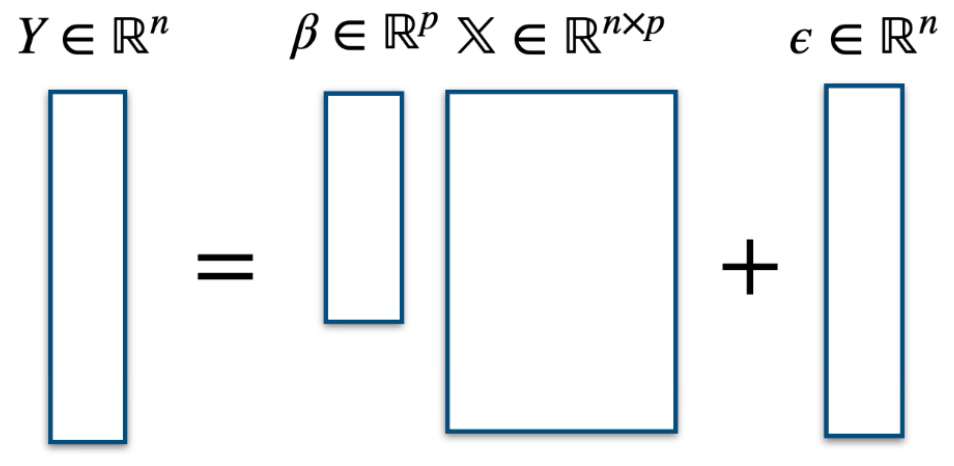
\includegraphics[width=0.4\textwidth]{linearmodel/mlm/matrix_not_mlm.png}
\end{figure}

To estimate the parameters we minimize the \textbf{Ordinary Least Squares}:
$$
    \hat{\beta} = \arg\min_{\beta\in\real^p} RSS(\beta) = \sum_{i=1}^n (y_i-x_i^T\beta)^2 = \left\|
    \mathbf{y}-\mathbf{X}\beta\right\|_2^2
$$
To do so we take the differential w.r.t. the parameters:
$$
    \frac{\partial}{\partial\beta} \|y-X\beta\|_2^2 = -sX^T(y-X\beta)=0 \Rightarrow \textcolor{red}{\hat{\beta} = (X^TX)^{-1}X^Ty}
$$

\subsection{Model assesment}
Under the \textit{Gaussian noise} assumption we have $\hat{\beta}\sim \mathcal{N}(\beta,\sigma^2(X^T
X)^{-1})$, giving us an estimator:
\begin{itemize}
    \item \textbf{unbiased} $\mathbb{E}[\hat{\beta}|X]=\beta$
    \item with \textbf{covariance} $Var(\hat{\beta}|X)=\sigma^2(X^TX)^{-1}$
    \item with \textbf{variance} $\hat{\sigma}^2=\cfrac{RSS}{n-p}$ (although is the same formul of simple linear regression, now we have less degree of freedom)
\end{itemize}
As for the simple linear regression, we could asses the model using the same tools:
\begin{itemize}
    \item std error $\text{SE}(\hat{\beta}_j) = \sqrt{\hat{\sigma}^2 [(X^\top X)^{-1}]_{jj}}$
    \item t-test for one parameter $H_0: \beta_j = 0, \quad t = \frac{\hat{\beta}_j}{\text{SE}
    (\hat{\beta}_j)}$
    \item confidence interval $\hat{\beta}_j \pm t_{n-p, 1-\alpha/2} \text{SE}(\hat{\beta}_j)$
\end{itemize}
Remeber that all the assesment are considered holding the other parameters fixed.

\newpage
\subsubsection{Variability explained}
\begin{figure}[h!]
    \centering
    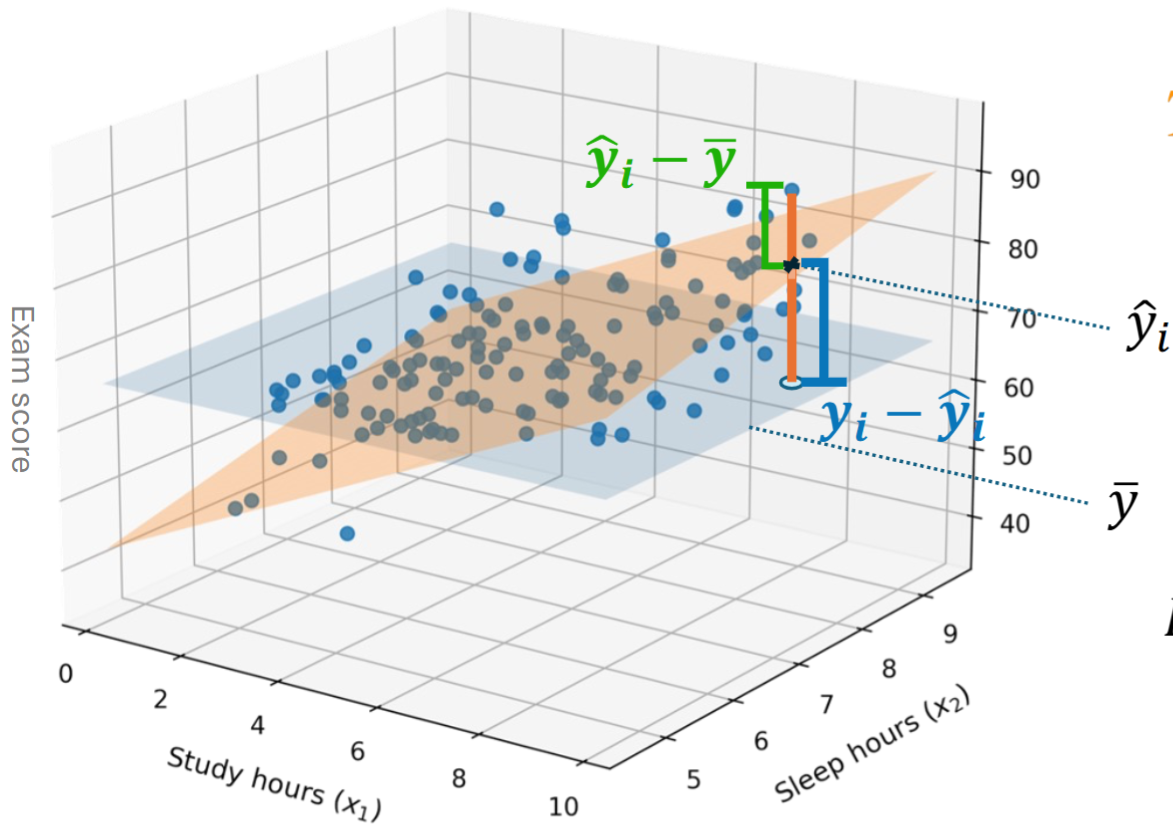
\includegraphics[width=0.5\textwidth]{linearmodel/mlm/mlm_var_explained.png}
    \caption*{
    As we could see, the concept and metrics remain the same as for simple linear 
    regressionm, therefore the extension to multiple predictor doesn't change this part.}
\end{figure}

\subsubsection{Model usefulness}
The concept is the same as for simple linear regression: the usefulness is measured in term of how
much our model links the predictors and the responses:
\begin{center}
    $H_0:\beta_0=\beta_1=\dots\beta_{p-1}=0$ vs $H_1: \exists i:\beta_i\ne 0$ \\
    $$
        F= \cfrac{ESS/(p-1)}{RSS/(n-p)} \sim F_{p-1,n-p}
    $$
\end{center}
W.r.t. simple linear regression now the F-test is no more equivalent to the t-test due 
the fact of testing many parameters jointly.\\
\vspace{0.2cm}
We could also think to test a reduced set of parameters $p_{red}$ called \textbf{nested 
model}: to compare the reduced model with the full model
\begin{center}
    $F= \cfrac{(RSS_{full}-RSS_{red})/q}{RSS_{full}/(n-p_{full})} \sim F_{q,n-p_{full}}$ with 
    $q=p_{full}-p_{red}$
\end{center}

\subsection{Multicollinearity}
The main issue with real data is that \textit{predictors are not independent}: we have 
\textbf{multicollinearity} := one predictor is highly predictable from the others.
We have \textbf{perfect collinearity} when the relationship is linear or \textbf{near 
collinearity} when the combination is almost linear (highly correlated features).

\vspace{0.2cm}
The multicollinearity problem is not something bad in general, it's a property of the data, but it means that the predictors are redundant, with all the unpleasant implications\\

\vspace{0.2cm}
Looking at the OLS estimator $\hat{\beta}=(x^TX)^{-1}X^Ty$, we see that it requires $X^TX$ to be invertible\arrow if there is multicollinearity within the matrix there are linearly dependent columns, making the matrix non-invertible.\\
If we think about it as a linear system we have that this implies $\infty$ solutions\arrow $Xv=0$ then $X(\beta+v)=X\beta$ giving us infinite fitted values.
When the data can't distinguish between $\beta$ from $\beta+v$ is said we have 
\textbf{ill-posedness}. How do we solve the issue? Drop a variable.

\newpage
If the predictors are \textit{near-collinear} we have that $X^TX$ is still invertible, but it's \textbf{ill-conditioned}: the inverse exists but it's numerically unstable, and if we look at the variance of our parameters $Var(\hat{\beta}|X)=\sigma^2 (X^TX)^{-1}$ \arrow this leads to large std error, wide 
confidence intervals ...\\
\begin{figure}[h]
    \centering
    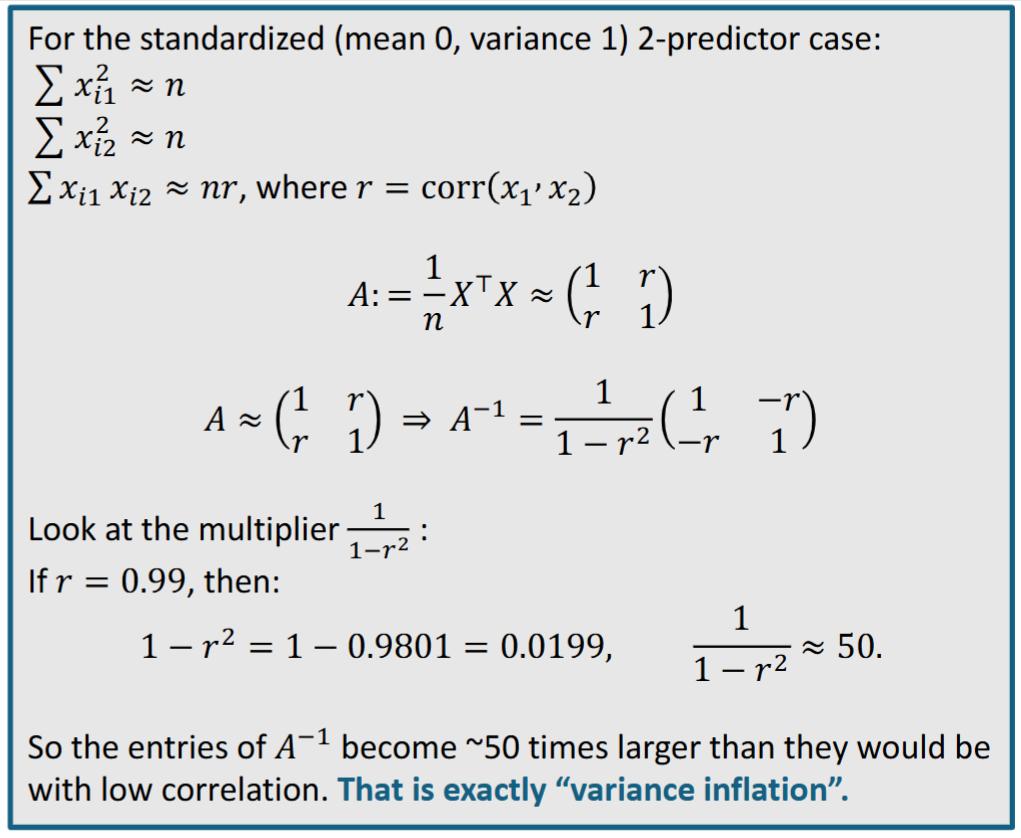
\includegraphics[width=0.5\textwidth]{linearmodel/mlm/var_inflation.png}
\end{figure}

However, we could have fitted values $\hat{y}=X\hat{\beta}$ pretty stable even with unstable params 
\arrow multicollinearity is much worse for intepretation/inference rather than for prediction (almost ever).

\paragraph{Variance Inflation Factor (VIF)}\hfill\\
How can we understand if some predictor might cause \textit{variance inflations}?

\vspace{0.2cm}
Take predictor $X_j$ and build a model that predicts $X_j$ from all the other predictor and consider this $R_j$, we have that
\begin{align*}
& \text{Var}(\hat{\beta}_j | X) = \frac{\sigma^2}{\sum_{i=1}^{n} (x_{ij} - \bar{x}_j)^2} \cdot \frac{1}{1 - R_j^2}\\
& \Rightarrow \textbf{VIF} = \frac{1}{1-R^2_j}
\end{align*}
If $R_j^2\rightarrow0\Rightarrow \text{VIF}\rightarrow\infty$ we see that the variance of the coefficient explodes, impling correlation between some predictors.

\subsubsection{How to deal with multicollinearity}
\begin{itemize}
    \item remove redundant predictors
    \item merge correlated predictors into one, changing its interpretability
    \item collect more data, hoping that by adding more variation we might be able to reduce colllinearity
    \item regularize (see later)
    \item apply PCA \arrow PCA regression (making the predictors independent by default)
\end{itemize}

\newpage
\subsection{Checking model assumptions}
Up to now we've made some assumptions about the error: $\mathcal{E}[\varepsilon|X]=0, Var(\varepsilon|
X)=\sigma^2, Cov(\varepsilon_i,\varepsilon_j|X)=0$ and on other aspects  of the model, but what if
this assumption doesn't hold?

\paragraph{Model linearity}
\begin{center}
    \textit{The model is linear in the coefficients} $\mathbb{E}[Y_i|X]=\beta_0+\beta_1x_{i1}
    +\beta_2x_{i2}$
\end{center}
\begin{figure}[h]
    \centering
    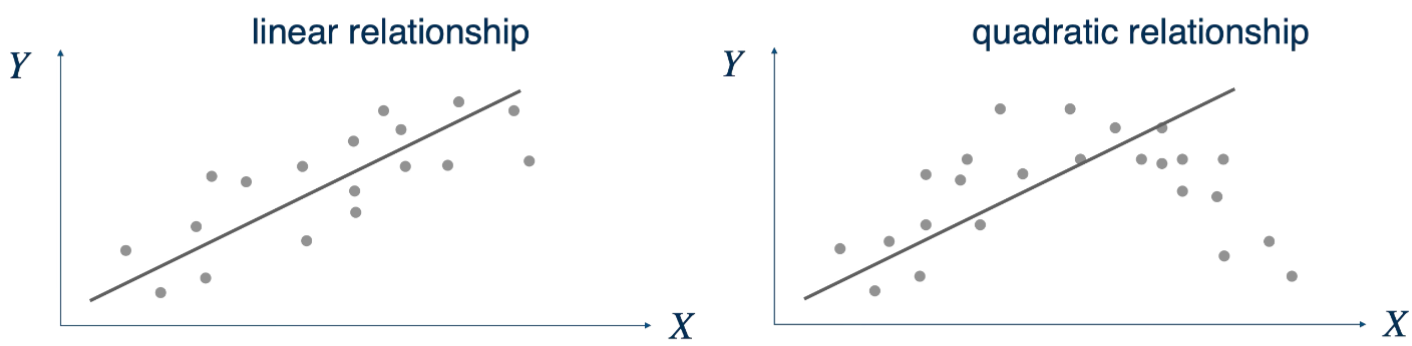
\includegraphics[width=0.5\textwidth]{linearmodel/mlm/lin_assumption.png}
\end{figure}
This doesn't mean that the predictors have to be linear, only the combination of predictors and parameters must be.

\paragraph{Null error mean}
\begin{center}
    $\expect[\varepsilon_i|X]=0$
\end{center}
meaning that there is no leftover information in the error and the errors are uncorrelated with the included predictors.\\
If this this assumption doesn't hold, we might have: variable bias, measurement errors in
predictors, bad model structure.

% if you figure out how to do it, do it
\begin{comment}
\begin{wrapfigure}[4]{l}{0.4\linewidth}
    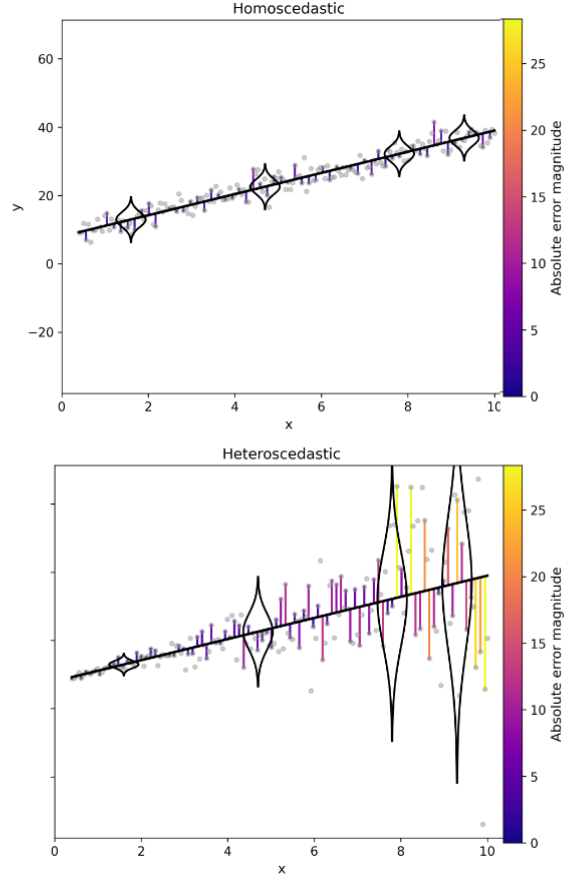
\includegraphics[width=0.9\linewidth]{linearmodel/mlm/homo_residual.png}
\end{wrapfigure}
\end{comment}

\paragraph{Homoscedasticity of residuals}
\begin{center}
    \textit{The error variance should be constant} $Var(\varepsilon_i|X)=\sigma^2$
\end{center} 
This means that the error should be spread roughly the same across the fitted model. If not, the 
OLS are still unbiased but the std may be wrong\arrow t-tests and CI might be misleading.
\begin{figure}[h!]
    \centering
    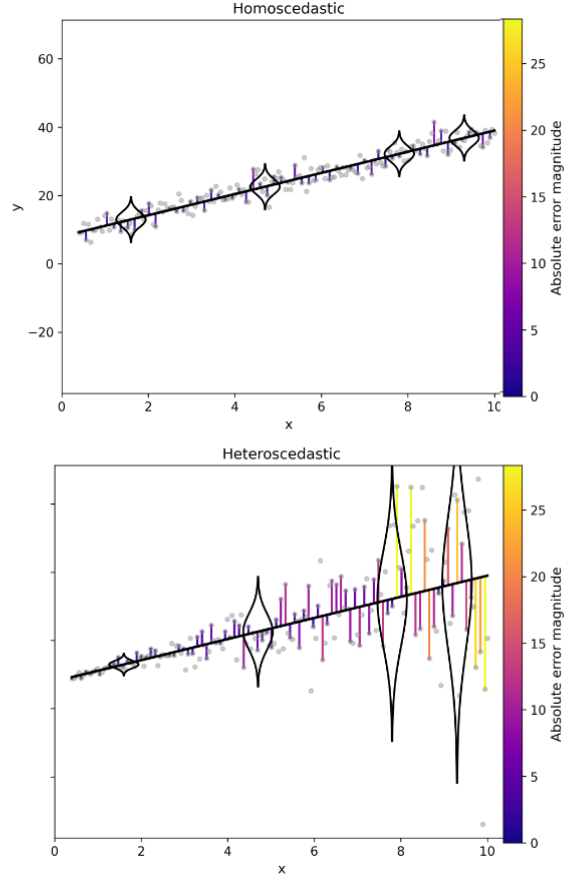
\includegraphics[width=0.3\linewidth]{linearmodel/mlm/homo_residual.png}
\end{figure}

\paragraph{Independence of errors}
\begin{center}
    \textit{Errors are independent} $Cov(\varepsilon_i,\varepsilon_j|X)=0\ \forall i\ne j$
\end{center}
If errors are correlated we get distorted std errors, inference might be wrong and the actual 
information within the datset is less than the sample size.\\
This kind of assumption often fails in a lot of realistic scenarios (time series, repeated
measures ...).

\paragraph{Independence of errors}
\begin{center}
    $\varepsilon_i \sim \mathcal{N(0,\sigma^2)}$
\end{center}
This assumption is not required for the OLS estimator rather than the simplicity of having
exact t-test, exact F-test, exact CI and exact PI. In larger samples mild deviations from
normal distribution are not problematic due CLT asymptotic result. 

\subsubsection{Leverage, outliers and influential points}

\paragraph{Leverage points}\hfill\\
Leverage points are those point extremely unusual in the predictors dimension. If we take a closer 
look to our prediction we have that $\hat{y}=X\hat{\beta} \xrightarrow[OLS]{} \hat{y}=X(X^TX)^{-1}
X^Ty=Hy$ where $H$ := \textbf{hat matix} \arrow $h_{ii}$ gives the \textbf{leverage} of the 
observations, in other words how unusual the observation is in the predictor space.\\ 
\vspace{0.2cm}
high leverage \arrow unusual combination\\
low leverage \arrow typical observation\\
\begin{figure}[h!]
    \centering
    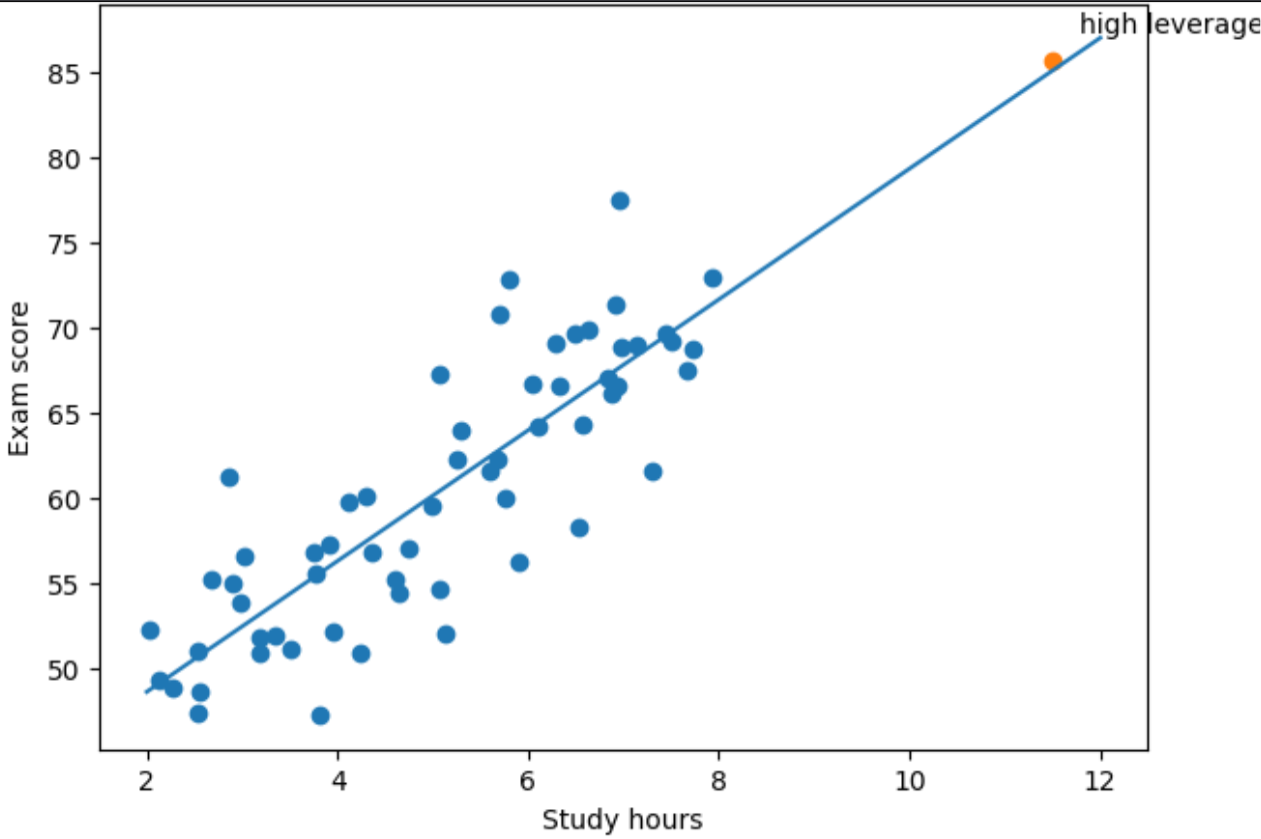
\includegraphics[width=0.6\textwidth]{linearmodel/mlm/leverage_point.png}
\end{figure}
High-leverage points following the regression model doesn't distort the model (they follow the 
exploited structure) but due them the regression line is strongly supported for extreme $x$, 
reducing the uncertanty in that region even if the information about it isn't that much, making CIs 
artificially tighter\arrow due them the model gives a false sense of generalization.

\newpage
\paragraph{Outliers}\hfill\\
Outliers are those observations that are unusual in the response, characterized by large residual
values $e_i=y_i-\hat{y}_i$. This can cause the increase of RSS, inflate the estimated noise level,
distort std error (with consequences on test and CI). Another thing is that this type of point 
might suggest possible data issues or model miss-specification.
\begin{figure}[h!]
    \centering
    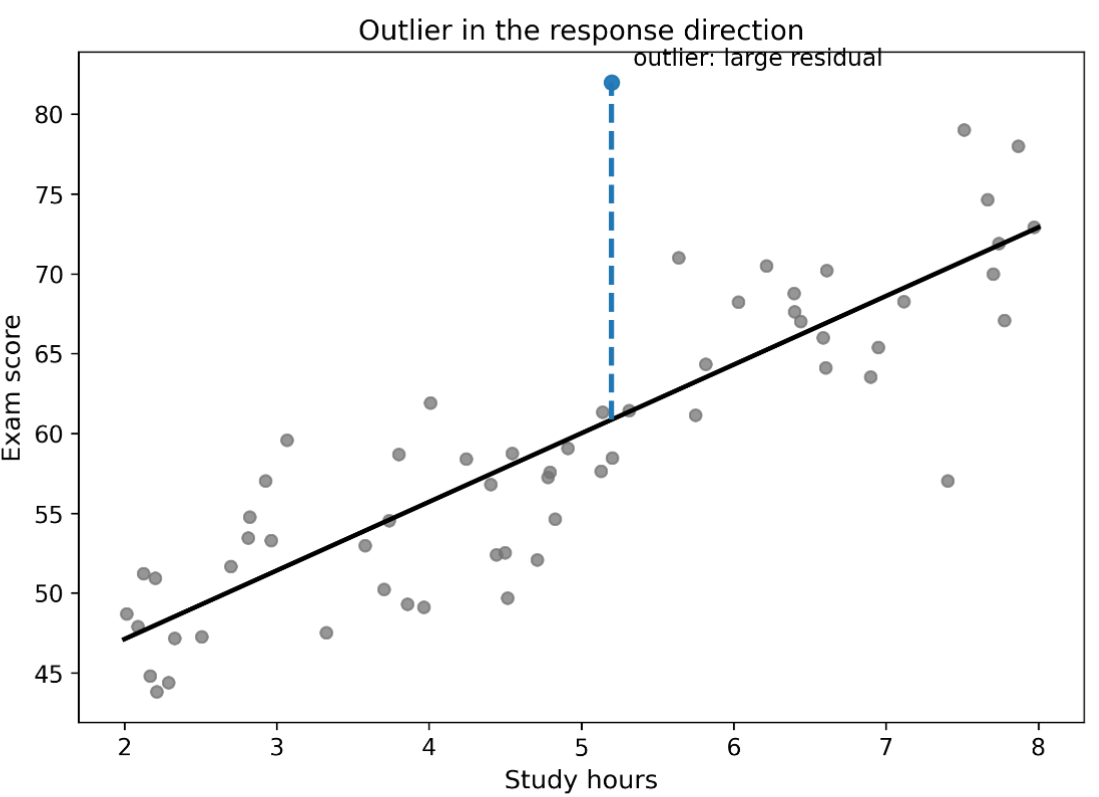
\includegraphics[width=0.6\textwidth]{linearmodel/mlm/outlier.png}
\end{figure}

\paragraph{Influential points}\hfill\\
\begin{center}
    high leverage + large residual \arrow influential point
\end{center}
This type of points might have big influence on the model, causing changes in the estimation of the
coefficients, distorted predictions and inference.
\begin{figure}[h!]
    \centering
    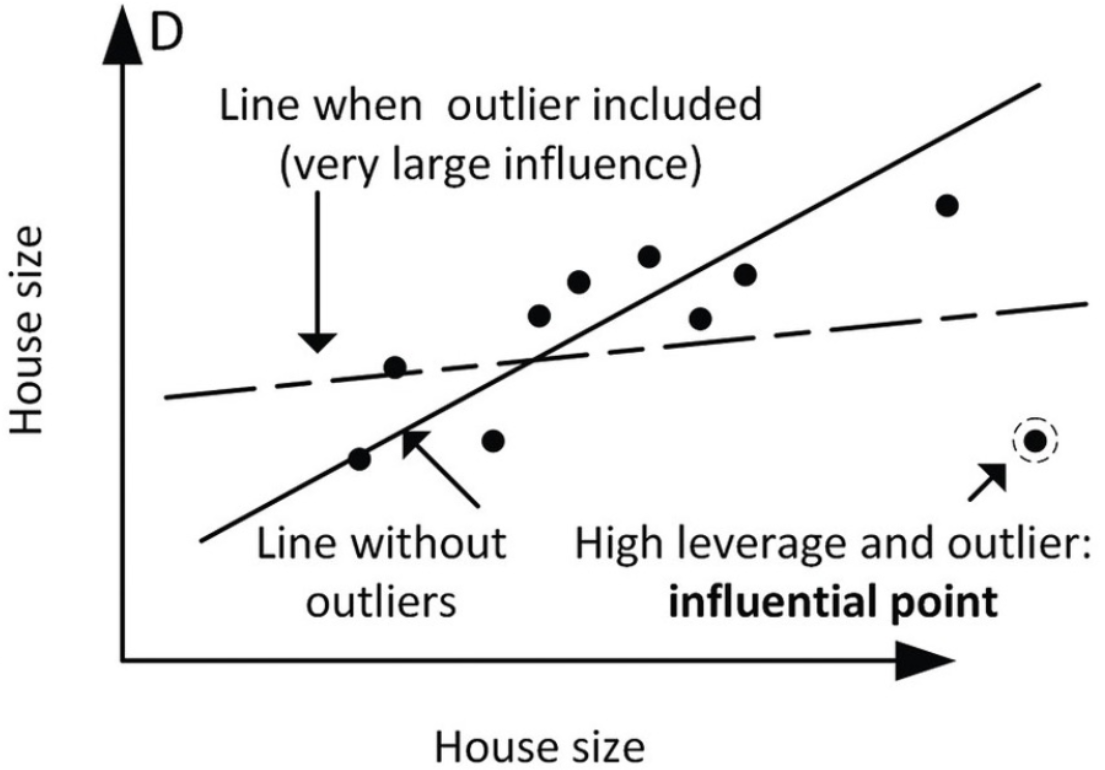
\includegraphics[width=0.6\textwidth]{linearmodel/mlm/influential_point.png}
\end{figure}

\newpage
\subsubsection{Residual vs fitted diagnostic plots}
\begin{figure}[h!]
    \centering
    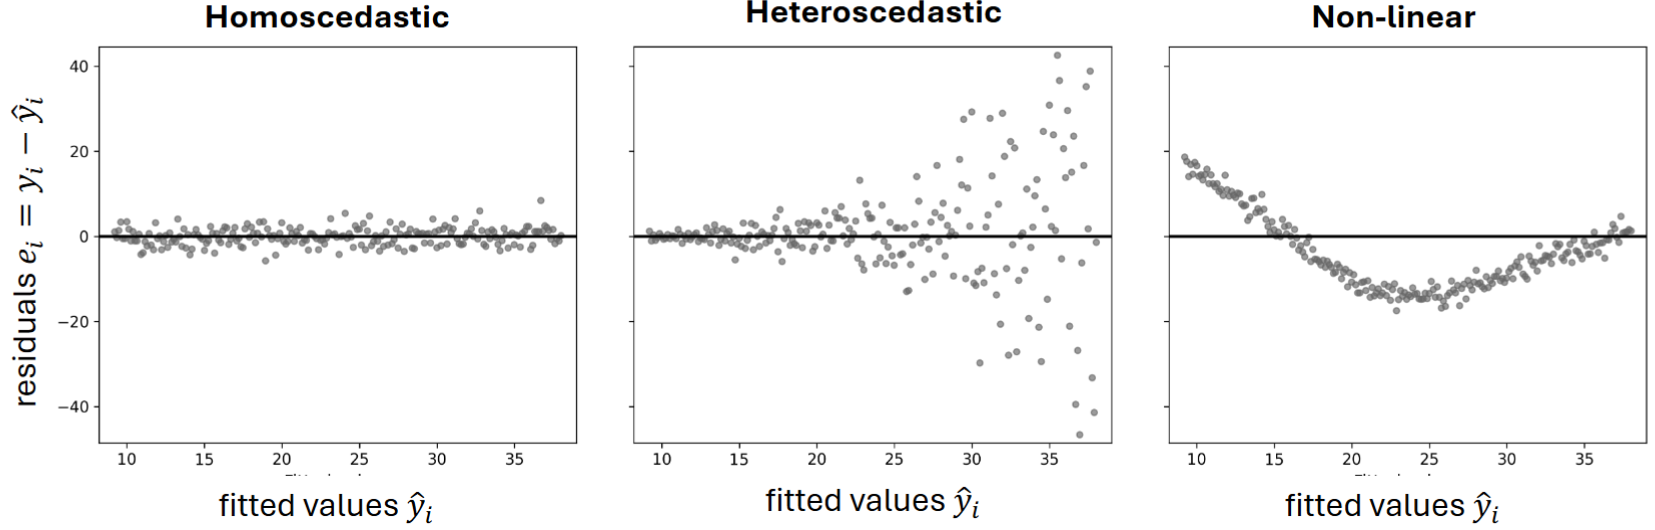
\includegraphics[width=0.8\textwidth]{linearmodel/mlm/resisual_vs_fitted_plot.png}
\end{figure}
Useful to check linearity of the mean, homoscedacity and possible outliers/leverage points.\\
\vspace{0.2cm}
\textcolor{green}{Good pattern}: andom cloud centered around zero, without visible structure.\\
\textcolor{red}{Bad pattern}: curved pattern (suggests nonlinearity), funnel shape (suggests 
heteroscedasticity), isolated points (possible outliers)\\

\subsubsection{Q-Q diagnostic plots}
\begin{figure}[h!]
    \centering
    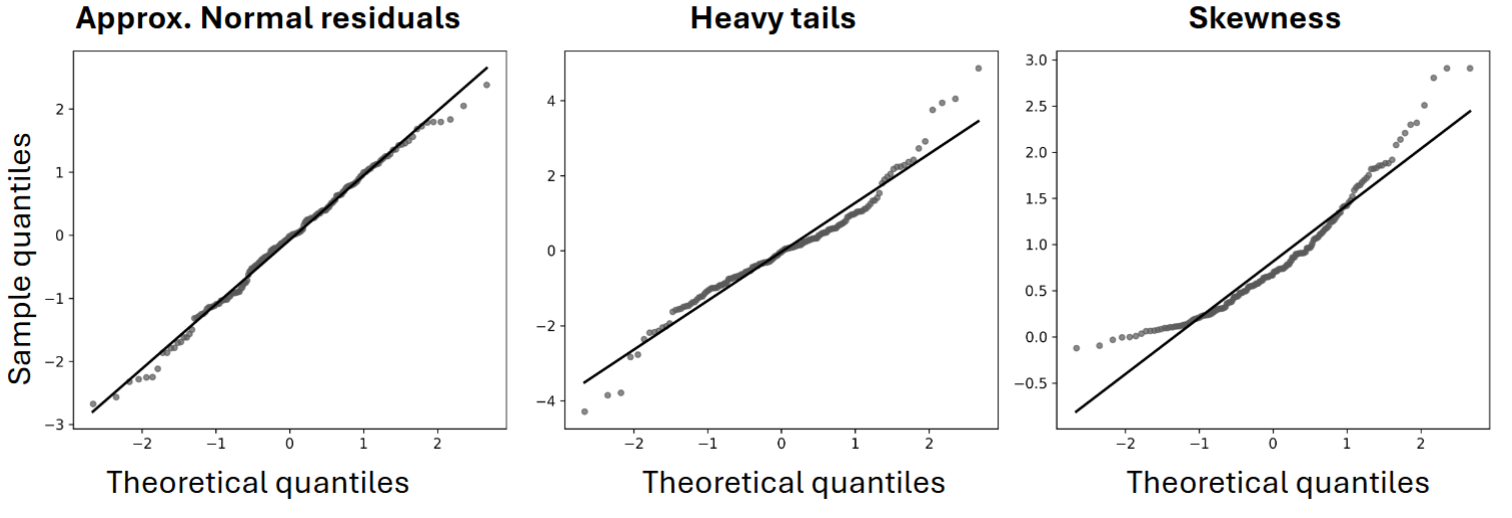
\includegraphics[width=0.8\textwidth]{linearmodel/mlm/qq_plot.png}
\end{figure}
Usefull to check whether residuals are approximately normal or not.\\
\vspace{0.2cm}
\textcolor{green}{Good pattern}: points close to the reference line, especially in the center.\\
\textcolor{red}{Bad pattern}: strong tail departures (extreme residuals), systematic asymmetry 
(skewness), s-shaped pattern (mismatch).\\

\subsubsection{Shapiro-Wlik test}
Standard test to check whether resisuals are normally distributed or not, to be used together with
Q-Q plot to strengthen it.
\begin{center}
    \textit{$H_0$: residuals are normal $\ H_1$: residuals are not normal}
\end{center}
large p-value \arrow no evidence against normality\\
small p-value \arrow residuals probably are not normally distributed.

\newpage
\subsubsection{Scale-location plots}
\begin{figure}[h!]
    \centering
    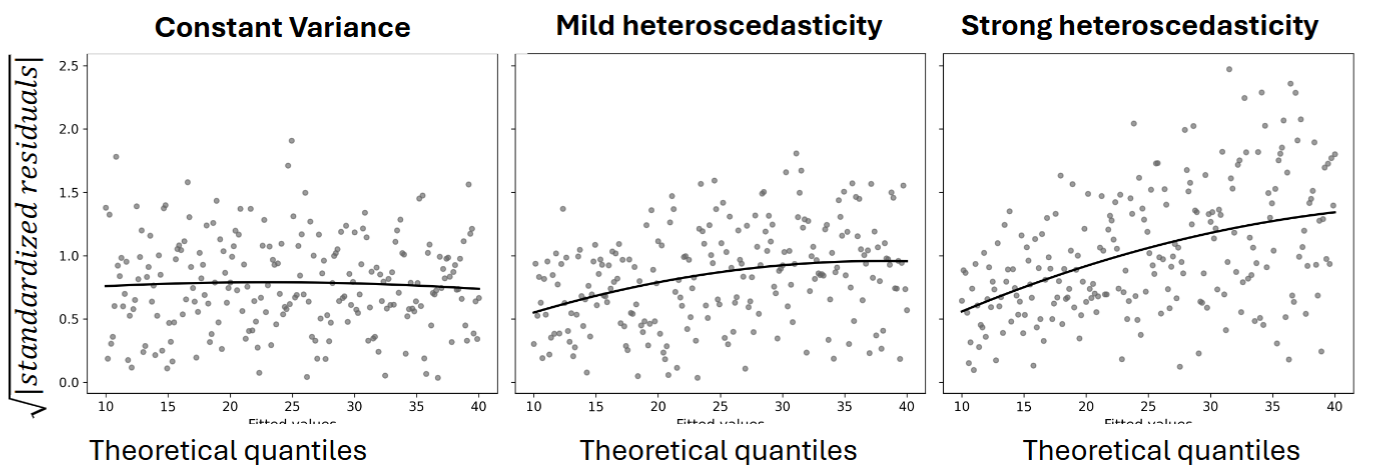
\includegraphics[width=0.8\textwidth]{linearmodel/mlm/scale-location_plot.png}
\end{figure}
Used to check for homoscedacity.\\
\vspace{0.2cm}
\textcolor{green}{Good pattern}: roughly horizontal band with uniform spread.\\
\textcolor{red}{Bad pattern}: increasing trend (variance grows with fitted values) or decreasing 
trend.

\vspace{0.4cm}
\subsubsection{Leverage vs studentized residuals}
Used to separate unusual $X$-values from unusual $Y$/values (in other words useful to highlight
leverage, outliers and influential points.)
\begin{figure}[h!]
    \centering
    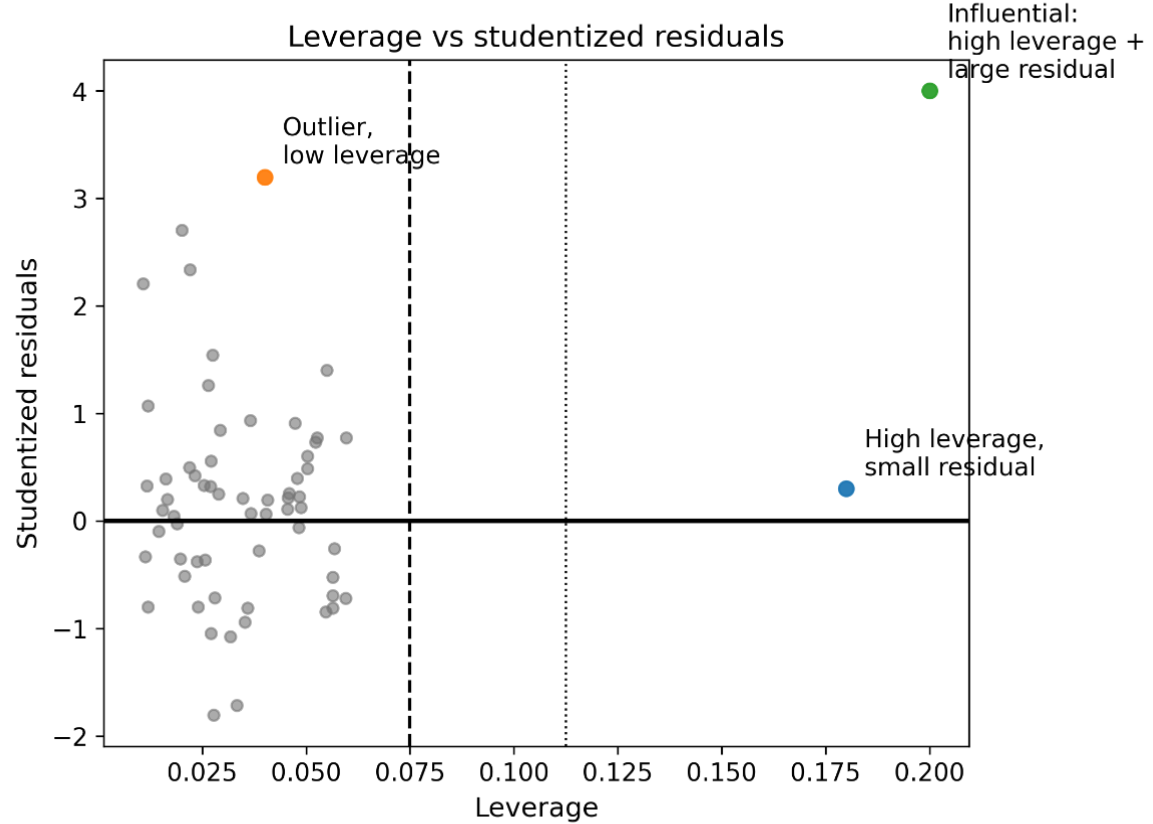
\includegraphics[width=0.7\textwidth]{linearmodel/mlm/lev_vs_stud_plot.png}
\end{figure}

\endgroup
\section{Logistic Regression}
In the linear regression we have a linear relationship between the target and the predictors, what if the relationship isn't linear? Let's assume our target is variable is a \textbf{binary variable}
$$
 Y_i=\begin{cases}
 1 & student\ i\ \ passes \\
 0 & student\ i\ \ fails
\end{cases}\ 
\Rightarrow
\prob (Y=1|X=x) = p
$$

If we try to use a linear regression model, we end up with something that ignores the real variable range. 
\begin{figure}[h]
    \centering
    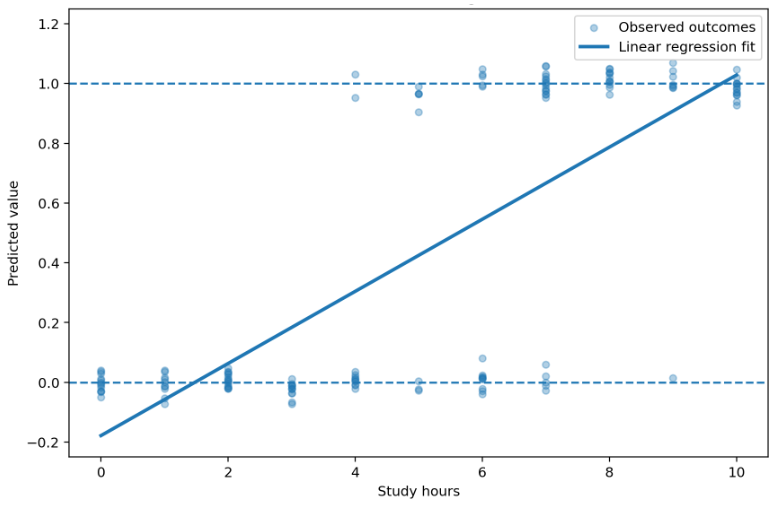
\includegraphics[width=0.3\linewidth]{img/logisticreg/linreg_exced_range.png}
\end{figure}

The idea is to solve the range issue is to change the undeling shape: we shift from the world of probabilities to the world of \textbf{odds} := how more likely is some event to happen with respect to not happen.
$$
 odds = \frac{p}{1-p}
$$
\begin{figure}[h]
    \centering
    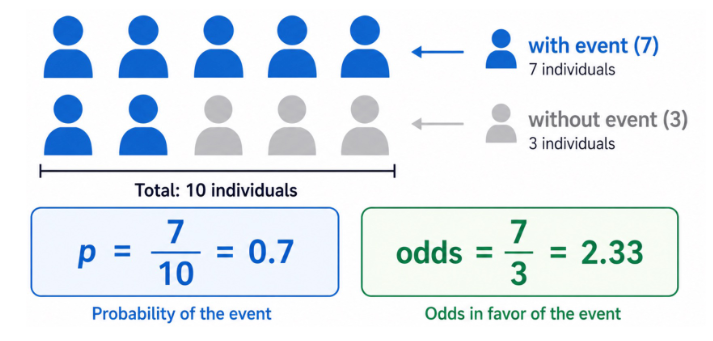
\includegraphics[width=0.3\linewidth]{img/logisticreg/odds_explained.png}
\end{figure}

and we then intepret them as follows:
\begin{itemize}
    \item $odds=1$ success and failure are equally possible
    \item $odds>1$ succcess is more probable than failure 
    \item $odds<1$ failure is more probabl than success
\end{itemize}

However we can't use the linear regression with odds since they are a non-negative measure (the won't never go below zero) \arrow we take instead the \textbf{log-odds/logit}
$$
 \log(odds) = \log\left(\frac{p}{1-p}\right)
$$
\begin{figure}[h]
    \centering
    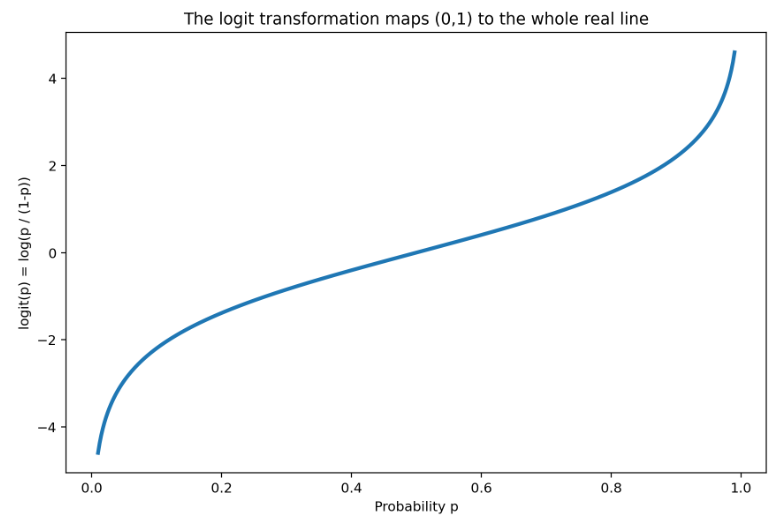
\includegraphics[width=0.3\linewidth]{img/logisticreg/logit_visualized.png}
\end{figure}

Now in this new \textit{log-odds} space we use linear regression:
\begin{align*}    
    & \log(odds) = \log\left(\frac{p}{1-p}\right) = \beta_0 + \beta_1x_{i1}\ ... + \beta_px_{ip}  \\
    & \rightarrow \frac{p_i}{1-p_i} = e^{\beta_0 + \beta_1x_{i1}\ ... + \beta_px_{ip}} \\
    & \rightarrow p_i = \cfrac{1}{1+e^{\beta_0 + \beta_1x_{i1}\ ... + \beta_px_{ip}}}
\end{align*}
so by doing to we get back the probability through the \textbf{linear regression applied within a sigmoid function} (the model is still linear, but in the log-odds scale):
$$
p_i = \sigma(\eta_i)=\sigma(\beta_0+\beta_1x_{i1}...+\beta_px_{ip})
$$
\begin{figure}[h]
    \centering
    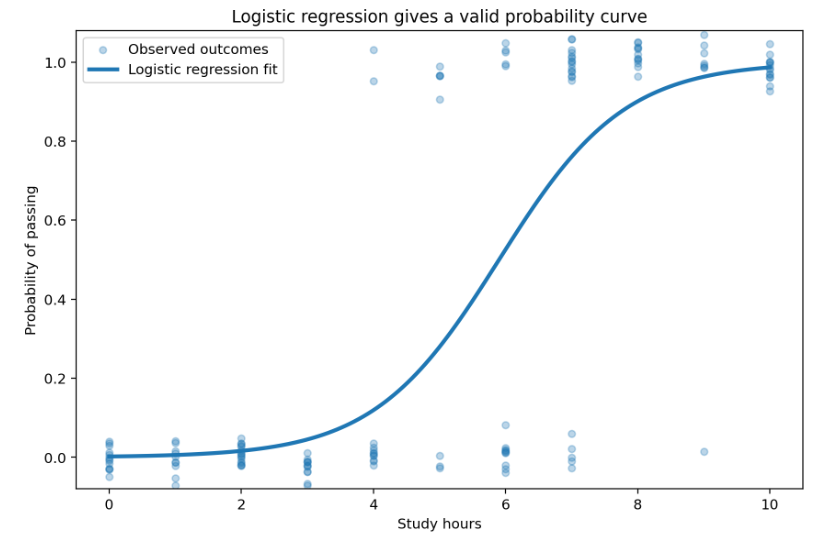
\includegraphics[width=0.5\linewidth]{img/logisticreg/logistic_regression.png}
\end{figure}\hfill\\
One of the advantages of this type fo regression is that it nevere crosses the 0, allowing us to intepret its value as a probability, and instead the extrems flatterns on [0,1]. Another good thing is that we are able to interpret the model:\\

\vspace{0.6cm}
\textbf{Coefficient's interpretation: categorical variables} \\
Our feature is somethign like this:
$$
 x_i=\begin{cases} 0 & GroupA\\ 1& GroupB\end{cases}\ 
\rightarrow \log\left(\frac{p_i}{1-p_i}\right) = \beta_0+\beta_1x_i
$$
to compare the two groups we have to subtract the fitted values:
\begin{align*}
& log\left(\frac{p_B}{1-p_B}\right)-log\left(\frac{p_A}{1-p_A}\right) = \beta_0+\beta_1-\beta_0 = \beta_1 \\
& \\
& \rightarrow \log\left(\frac{p_b/(1-p_B)}{p_A/(1-p_A)}\right)=\beta_1
\end{align*}
$\Rightarrow$ the odds-ratio is equal to the slope in the log-odds space.

\newpage
\textbf{Coefficient's intereptation: continuous variables}\\
If instead we consider a continuous predictor we get
\begin{align*}
& \log\left(\frac{p(x)}{1-p(x)}\right)=\beta_0+\beta_1x,\ \log\left(\frac{p(x+1)}{1-p(x+1)}\right)=\beta_0+\beta_1(x+1) \\
& \\
& \rightarrow \log\left(\frac{odds\ at\ x+1}{odds\ at\ x}\right) = \beta_1
\end{align*}

Also in the continouous case $e^{\beta_1}$ is the odds-ratio for single-unit increase. 
In general we can deduce that the increase is constant in the log-odds space:
\begin{figure}[h!]
    \centering
    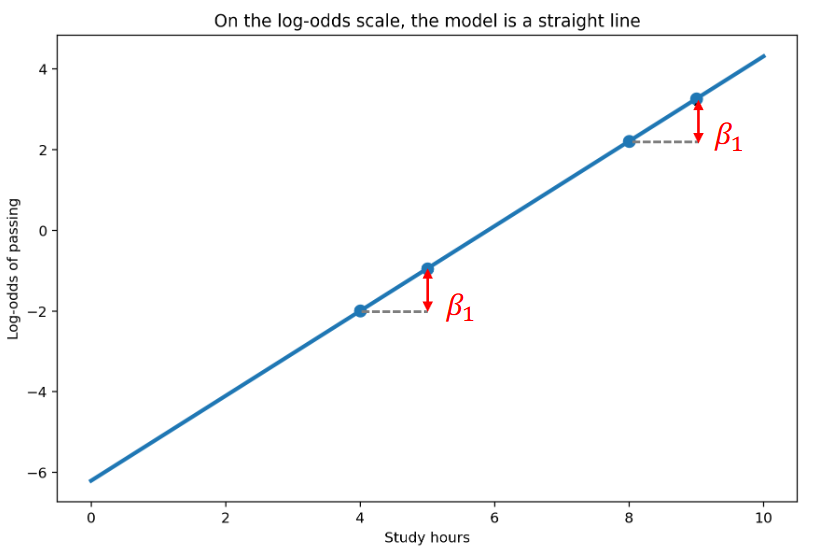
\includegraphics[width=0.4\linewidth]{img/logisticreg/logodds_slope.png}
\end{figure}

The the effect in the odds space is still constant $e^{\beta_1}$, but visualized as an exponential:
\begin{figure}[h]
    \centering
    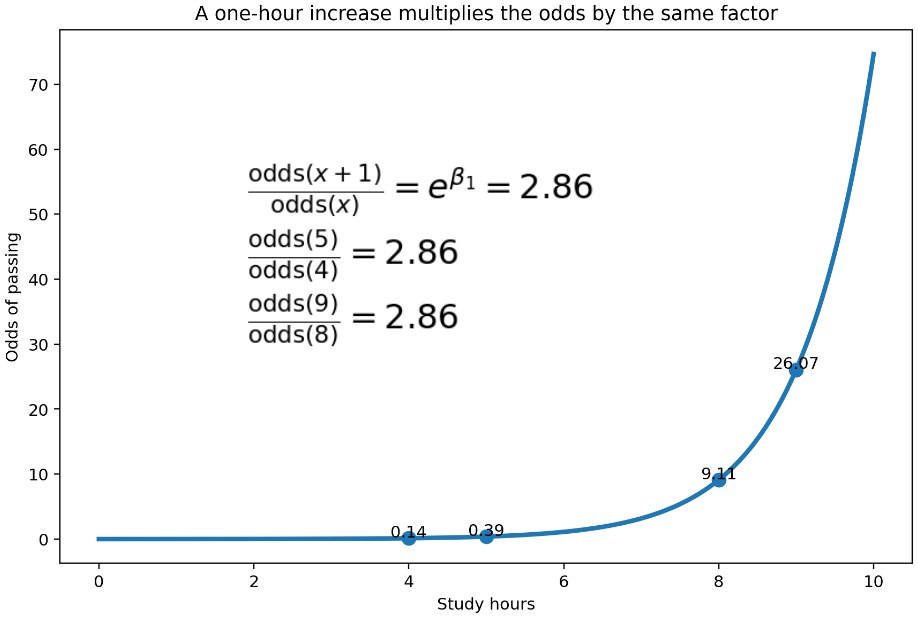
\includegraphics[width=0.4\linewidth]{img/logisticreg/odds_slope.png}
\end{figure}

On probablities instead the ratio is not constant, but dependes on where the position on the logistic curve:
\begin{figure}[h]
    \centering
    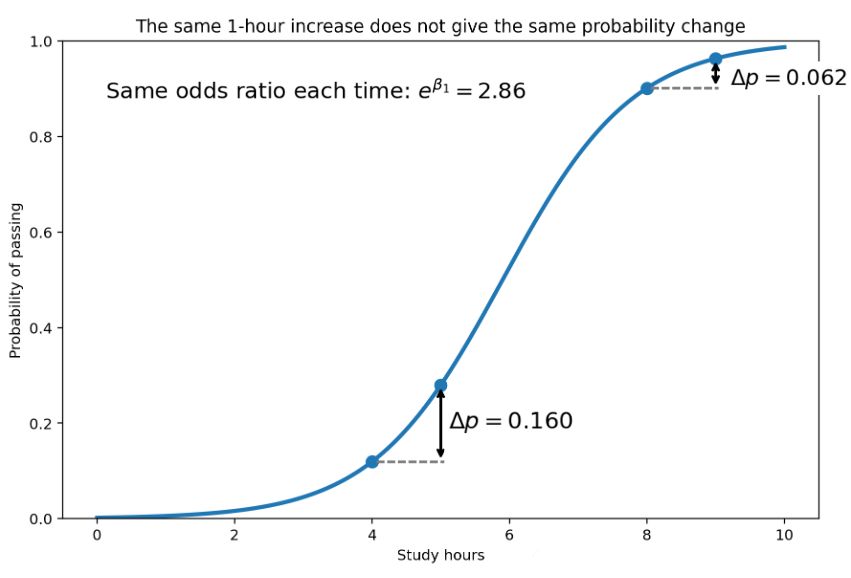
\includegraphics[width=0.5\linewidth]{img/logisticreg/prob_logreg_slode.png}
\end{figure}

\newpage
% --------------------------------------------------------------------------------------------------------
\subsubsection{Generalized Linear Models (GLM)}
Linear regression is a specific case of GLM, which is a generalization of linear regression that links the linear model with the response through a non-linear \textbf{linking function} $g$.

We can always identify three elements:
\begin{enumerate}
    \item random response variables
    \item linear model of the predictors $\eta_i=\beta_0+\beta_1x_{i1}...+\beta_px_ip{}$
    \item linking function $g(\mu_i)=\eta_i$ where $\mu_i=\mathbb{E}[Y_i|X_i]$
\end{enumerate}
To get the basic linear regression model from GLMS, we can take $g()=Id$


% --------------------------------------------------------------------------------------------------------
\vspace{0.3cm}
\subsection{Classification models (classifiers)}
The logistic regression doesn't give a label directly, instead its output is the probability of that label: $\hat{p}_i=\mathbb{P}(Y_i=1|X_i)$.
To get some kind of \textbf{classification rule} we have to set a \textit{treshold} $t\in (0,1)$
$$
\hat{Y}_i=\begin{cases}
    1 & \hat{p_1}\ge t \\
    0 & \hat{p_1}< t 
\end{cases}
$$
\begin{figure}[h]
    \centering
    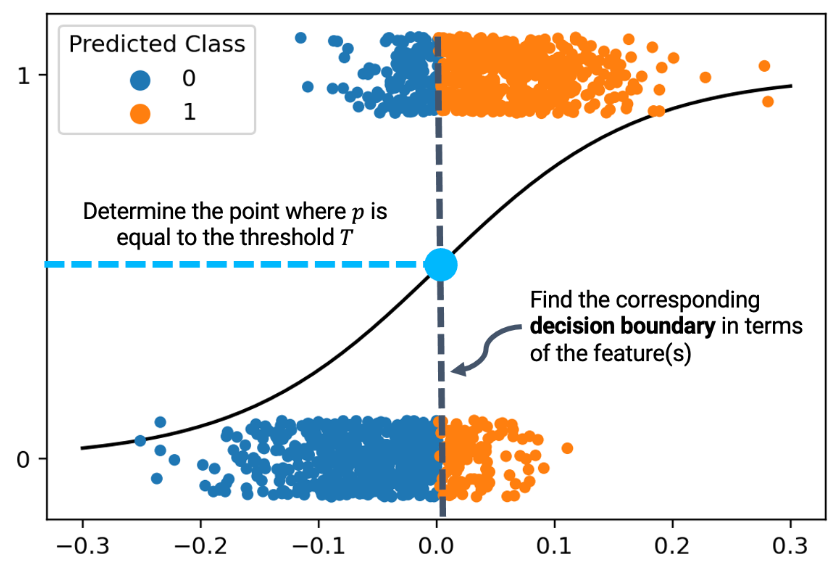
\includegraphics[width=0.4\linewidth]{img/logisticreg/logreg_classificator.png}
\end{figure}

\paragraph{How to choose the threshold}
The most common choice is taking $t=0.5$, however is really context-dependent: if we'd like a model more selective/conservative we should take a high treshold.
Sometimes when the datset is \textit{unbalanced} it might be a good idea to set the treshold to the relative frequence of the minority class. Another suggestion is to use the \textit{negative class} frequency (by convention the case $0$ is the negative class) . Otherwise there is also the \textit{Youden's J index} which suggest of using $TPR -FPR$ (see later what this values are).

% --------------------------------------------------------------------------------------------------------
\vspace{0.3cm}
\subsection{Model assumption of linear regression}
Some assumption made for the linear regression moels are relaxed, for the logistic regression usually we assume that:
\begin{itemize}
    \item observations are independet
    \item only important/meaningful predictors are included, irrelvant ones arent't added
    \item there is no multicollinearity
    \item the logit event probability is linear in the predictors
    \item there is no \textbf{perfect separation} := there is no variable that divides perfecly the dataset in classes
\end{itemize}

\newpage
However we can handle easily also \textbf{interactions among predictors} (bilinear relationships).\\
If we take as exmaple $x_{i1}$ = study hours, $x_{i2}$ = good/bad sleep we get as model
$$
\log\left(\frac{p_i}{1-p_i}\right)=\beta_0+\beta_1 x_{i1} +\beta_2 x_{i2} +\beta_3 x_{i1} x_{i2}
$$
by fixing the value of one varibale we can study the behavior of the model when the other predictor changes, obtaining two different reduced models with \textit{diffrent slopes}
\begin{figure}[h]
    \centering
    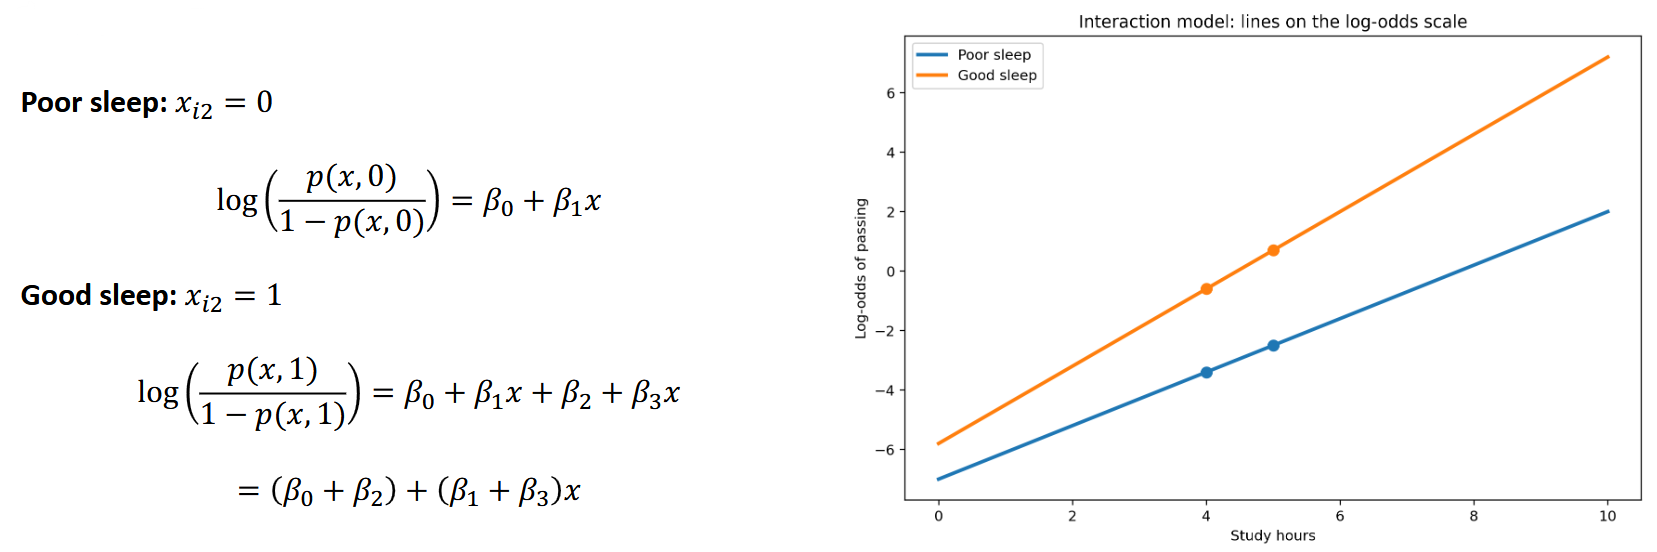
\includegraphics[width=0.8\linewidth]{img/logisticreg/partial_model.png}
\end{figure}\hfill\\
this different slope in the log-odds space is reflected also in the probability space, getting two different probability curves:
\begin{figure}[h]
    \centering
    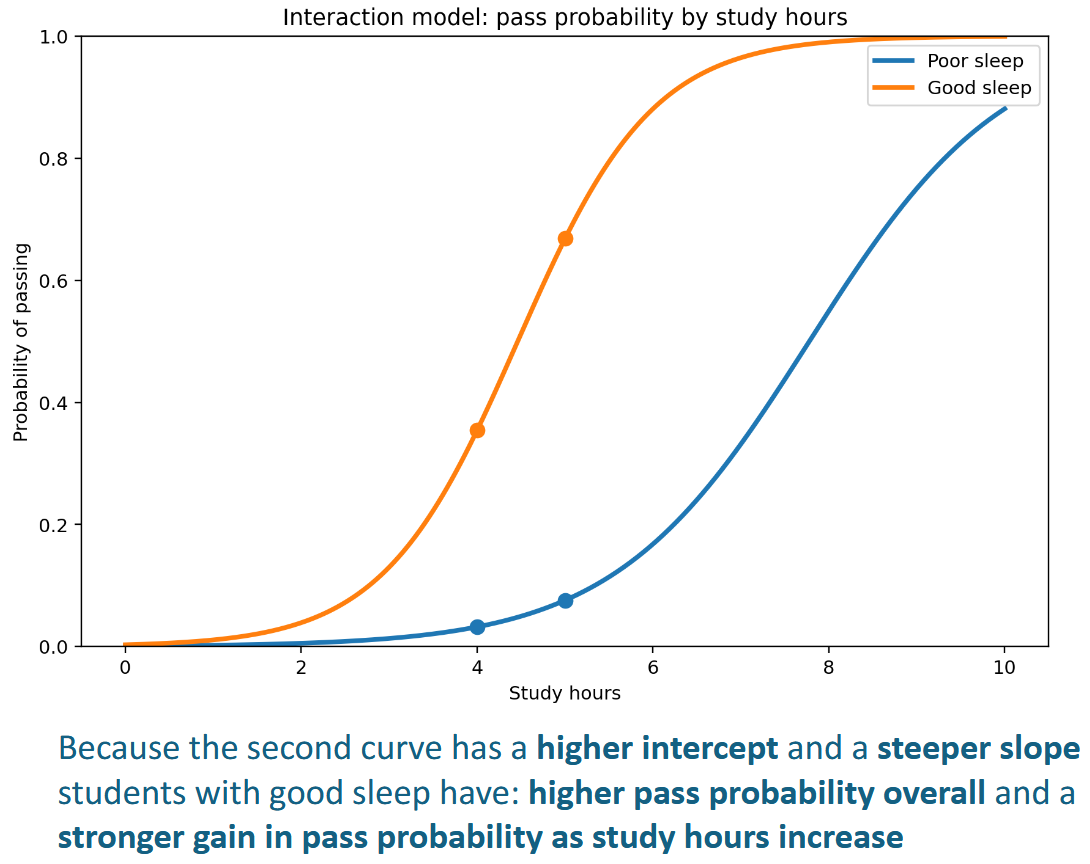
\includegraphics[width=0.5\linewidth]{img/logisticreg/logreg_probs_interacting_vars.png}
\end{figure}

% --------------------------------------------------------------------------------------------------------
\vspace{0.3cm}
\subsection{Logistic model estimation}
Since our predictors are binary $\{0,1\}\ni Y_i \sim Bernoulli(p_i)$ we have that $\prob(Y_i=y|X_i)=p_i^{y}(1-p_i)^{1-y}$ \arrow a good model should assing high probability to the outcomes that actually occurred and low to those not occurred \arrow a good model chooses $\beta$s so that the observed pattern are as plausible as possible.\\ 
To estimate the model we use MLE as always:
$$
L(\beta)= \prod_{i=1}^np_i^y(1-p_i)^{1-y} \rightarrow \ell(\beta)=\log L(\beta) = \sum_{i=1}^n y\log p_i + (1-y)\log (1-p_i
$$

\newpage
\subsubsection{Estimation with perfect separation}
Perfect separation occours when some predictor divides the two classes completely. While might looks like a good thing, it's a little bit tricky for the MLE: likelihood makes the logistic curve steeper and steeper, approaching the step function, and this would require the estimation of an infinite estimator, which is not possible with MLE.
\begin{figure}[h]
    \centering
    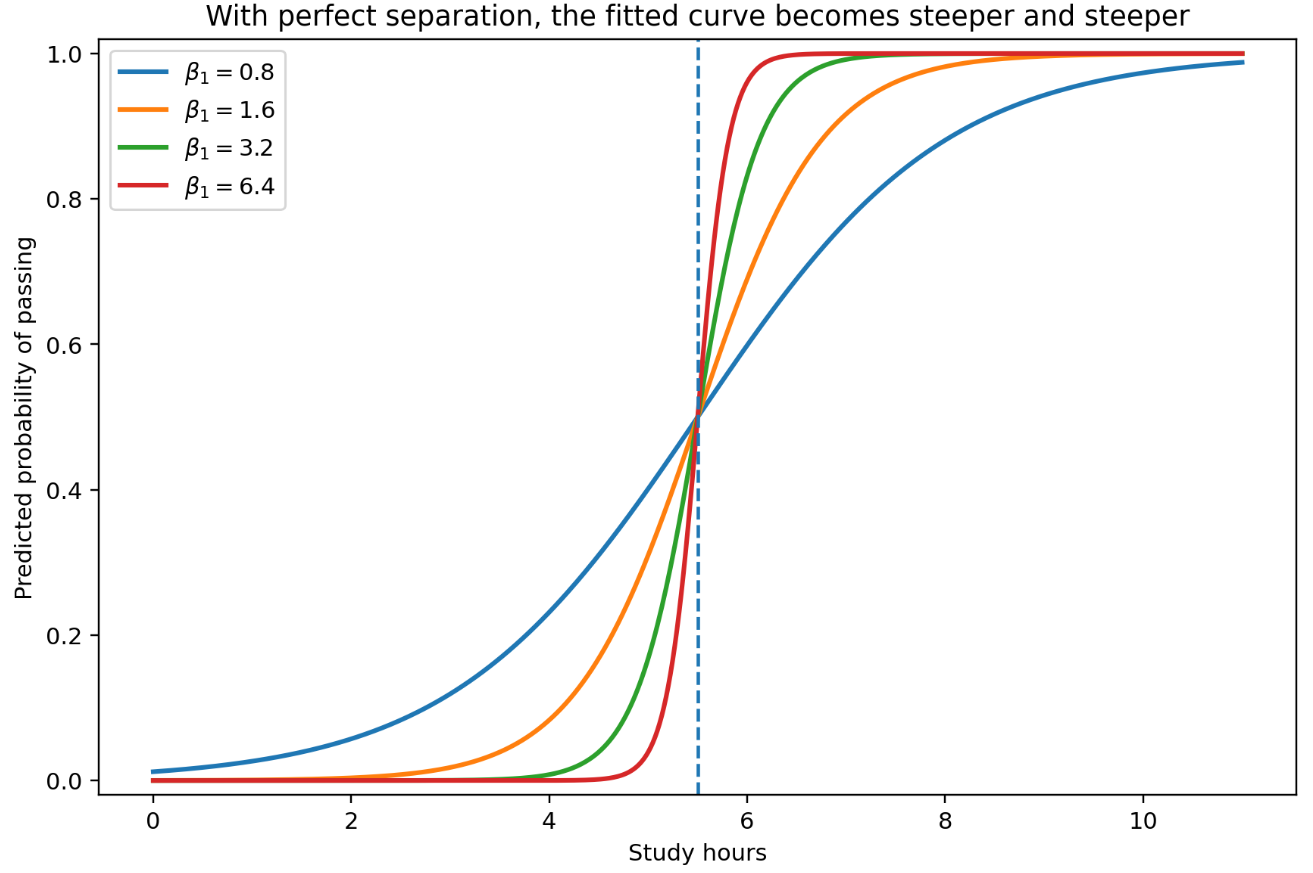
\includegraphics[width=0.4\linewidth]{img//logisticreg/mle_perfect_sep.png}
\end{figure}
\hfill\\
Similar situation for the \textbf{quasi-complete separation} := most predictors are perfectly separated but a small group overlap. In this setting the fitted coefficients might suffer from unstability.\\
\hfill\\
In the case of (quasi)perfect separation software might fail to converge, return extremely large coefficients with large std errors, or in some cases even warnings. To avoid these isseus we can try to collect more data, simplifying the model, combine/remove sparse categories or use penalized logistic regression (logistic regression that adds penalties in the loss function to avoid overfitting).

% --------------------------------------------------------------------------------------------------------
% give another look to this
\vspace{0.3cm}
\subsection{Model usefulness assessment}
A first approach to measure our model's performance is compare it with the purely-random/intercept-only predictor. As metric for the comparison we use the \textbf{likelihood ratio test} 
$$
2(\ell_{full}-\ell_{null})
$$ 
where $full$ stand for our model and $null$ for the intercept-only \arrow the larger the better. The 2 is only to fit the statistic in a Chi-squared distribution.\\

\vspace{0.5cm}
Another metric to evaluate our model il the \textbf{deviance} $-2\ell$ where $\ell$ is the log-likelihood, so the larger the better.\\
This statistic is useful when we want to compare two nested models.

\vspace{0.5cm}
Another metric used to compare out model with the intercept-only one we can also use the \textbf{McFdadden's pseudo-$R^2$}
$$
R^2_{McFadden}  = 1 -\cfrac{\ell_{full}}{\ell_{null}}
$$

After general model fitting estimation, we'd like to know whether each predicotr contributes or not: to do so we use statistic tests: $H_0:\beta_j=0$ vs $H_1:\beta_j\neq0$\\
A common used statistic is
$$
z=\cfrac{\hat{\beta}_j}{SE(\hat{\beta}_j)}
$$
if the values is large then the realtive p-value is low, giving strong evidence that the predictor is meaningful. As usual, if we build a confidence interval we get $\hat{\beta}_j \pm z_{1-\alpha/2}\ SE(\hat{\beta}_j)$ and this interval contains zero, the coefficient might be absent.
However this is for the log-odds, for the odds realm we have to make it exponential:
$$
\hat{\beta}_j \rightarrow e^{\hat{\beta}_j},\ \left[e^{\hat{\beta}_j^L}\ ,\ e^{\hat{\beta}_j^U} \right]
$$
if this interval in the odds world contains 1 hten the coefficient might be irrelevant.

% --------------------------------------------------------------------------------------------------------
\subsection{Classifier performance}
We can resume the outcome ouf our classfier in a \textbf{confusion matrix}: it resumes the outcome of the model in predicting the datapoint classification.
\begin{figure}[h]
    \centering
    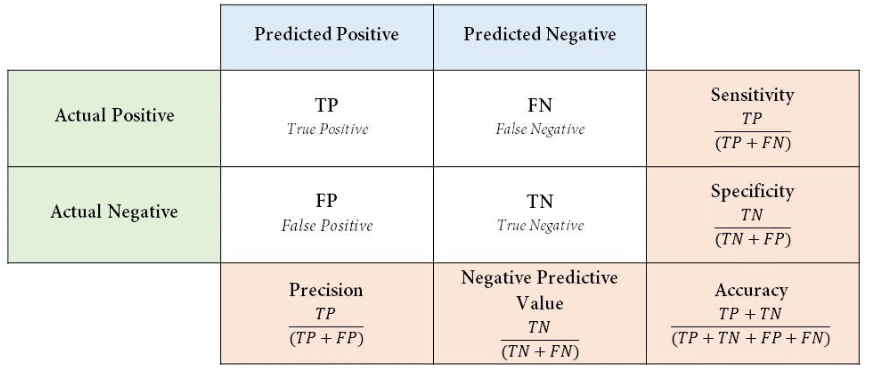
\includegraphics[width=0.6\linewidth]{img/logisticreg/classifier_performance.png}
\end{figure}\hfill\\
\textbf{Accuracy} := raw number of good evaluation, a little bit silly since is influenced by how much tha dataset is unbalanced.

% take the last 5-10 minutes of the recording in which she's talking about the ROC curve and AUC index, plus

We could see that these values are dependent from the threshold chosen. We could think of maximizing the model selection based on the maximization of accuracy.

To remove this dependecy we can take the area of this curve.

This type of evaulation for classification model has some drawbacks: it requires amodel that uses probabilities as output.
% -----
Other metrics are 
$$\text{Recall} = \text{Sensitivity} = \frac{TP}{TP+FN}$$
$$\text{F1-Score} = \frac{2 \cdot \text{Precision} \cdot \text{Recall}}{\text{Precision} + \text{Recall}}$$
$$\text{Specificity} = \frac{TN}{TN+FP}$$
\section{Multinomial Logistic Regression}
This kind of problem is the generalization of classical \textit{logistic regression} in which we have $K$classes, assuming one class as \textit{baseline} (take the K-th class without loss of generality) and building up the model with the other classes:
\begin{align}
&\prob(y = k | x) = \frac{e^{\beta_{k0} + \beta_{k1} x_1 + \beta_{k2} x_2 + \dots + \beta_{kp} x_p}}{1 + \sum_{j=1}^{K-1} e^{\beta_{j0} + \beta_{j1} x_1 + \beta_{j2} x_2 + \dots + \beta_{jp} x_p}} \quad\text{for }k < K \\
&\prob(y = K | x) = \frac{1}{1 + \sum_{j=1}^{K-1} e^{\beta_{j0} + \beta_{j1} x_1 + \beta_{j2} x_2 + \dots + \beta_{jp} x_p}} = 1 - \sum_{k=1}^{K-1} \prob(y = k | x)
\end{align}
iso now for each variable we have a set of coefficients, one for each class. The baseline class will remain without a parameters, but we can choose it.
Now we can compute the 
$$
\log\left(
\frac{P(y = k \mid x)}
     {P(y = K \mid x)}
\right)
=
\beta_{k0}
+
\beta_{k1}x_1
+
\beta_{k2}x_2
+
\dots
+
\beta_{kp}x_p
\qquad \text{for } k = 1, \dots, K-1
$$
\section{K-Nearest Neighbour (KNN)}

Classification (in a general way) is a supervised learning task in which we try to assign to each sample $x_i$ a \textbf{class label} $y_i$ \arrow the key idea is to separate the feature space in classes.
\vspace{0.2cm}
The goal is to learn a model $f(x)\rightarrow \hat{\prob}(Y=y|X=X)$ and then shift from probabilites to predicting labels \arrow classification is both a prediction problem and a decision problem.

The simplest example of classification model is the \textbf{linear classfier}, which draws a line in the middle of the feature space, dividing the whole data space in two classes.
\begin{figure}[h]
    \centering
    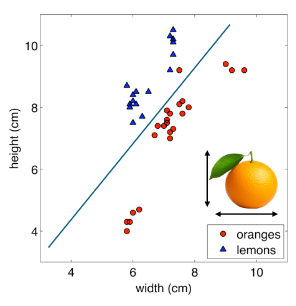
\includegraphics[width=0.2\linewidth]{img//classification//knn/class_lin_example.png}
\end{figure}
The \textit{logistic regression} IS a linar classfier, in fact creates a raw linear division of the log-odds space. The problem is that often the boundaries between classes are non-linear, then requiring to shift toward more complex models \textcolor{gray}{(this idea of dividing the feature space in decisionr regions is common to all classification algorithms)}.

\subsection{K-Nearest Neighbor (KNN)}
The idea behind this is that \textit{similar observations should have similar labels}. 
To classify a new observation we take the $k$-closest training datapoints and predict the new point with the most frequent label. The Euclidean distance is a common choice.
$$
x^* = \arg\min_{x_j\in \text{train set}} d(x_0,x_i)
$$
\vspace{0.2cm}
This type of algorithm is an \textbf{instance-based learning}: the training data is stored and it's actualy used for the prediction. It's also a \textbf{lazy learner}: all the computation is made at prediction time.

\textcolor{green}{\textbf{Pro:}}
\begin{itemize}
    \item extremelly simple
    \item no assumption on the parameters
    \item very flexible, complex shapes may arise
\end{itemize}
\textcolor{red}{\textbf{Cons:}}
\begin{itemize}
    \item extremelly sensitive to noise (one single misprediction might cause huge problems), risk of overfitting
    \item computational expensive at predict time
    \item sensitive to irrelevant features
\end{itemize}

The $k$ at the end is just an hyperparameter and finding the right $k$ is a \textbf{model-selection problem}.
\begin{figure}[h]
    \centering
    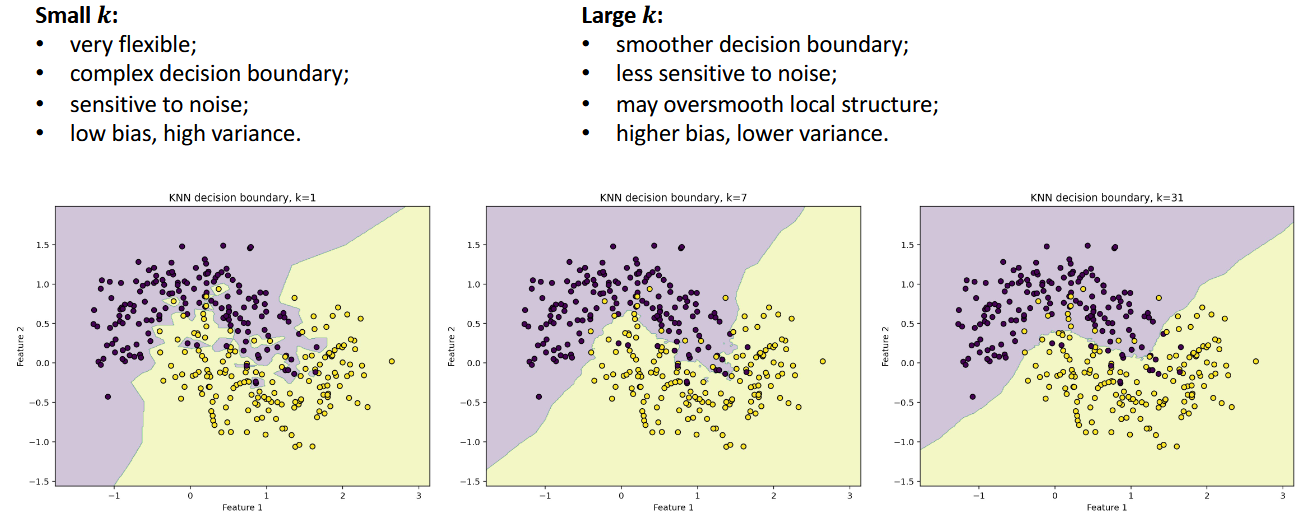
\includegraphics[width=0.5\linewidth]{img//classification//knn/k-neighbour-choice.png}
\end{figure}

\section{Model assesment \& selection}

\textcolor{gray}{The following considerations hold for all supervised learning methods, for simplicity we'll focus on classification methods.}
\vspace{0.2cm}
Once we've trained a classifier we're interested in evaluating the model on new observations drawn from the same population.

We have some data model $\mathcal{D} = \{(x_i, y_i)\}_{i=1}^n$ on which we train a model $\hat{f}_{\mathcal{D}}(x)$.\\
To evaluate our model we need to known the error it will make on future data, in other words we want the \textbf{expected misclassification error}:
$$
Err = \expect_{(X,Y)}[L(\ Y,\ \hat{f}_{\mathcal{D}}(X)\ )]
$$
where $L$ is a simple \textbf{loss function} returning 0 if the prediction is correct 1 otherwise.\\

To do this we take an independent set to \textbf{test our model} $\mathcal{D}_{test} = \{(x_i, y_i)\}_{i=1}^m$ and on this new dataset we compute the misclassification error:
$$
\widehat{Err}_{test} =  \frac{1}{m}\sum_{i=1}^{m} L(y_i, \hat{f}_{\mathcal{D}}(x_i))
$$
\begin{figure}[h]
    \centering
    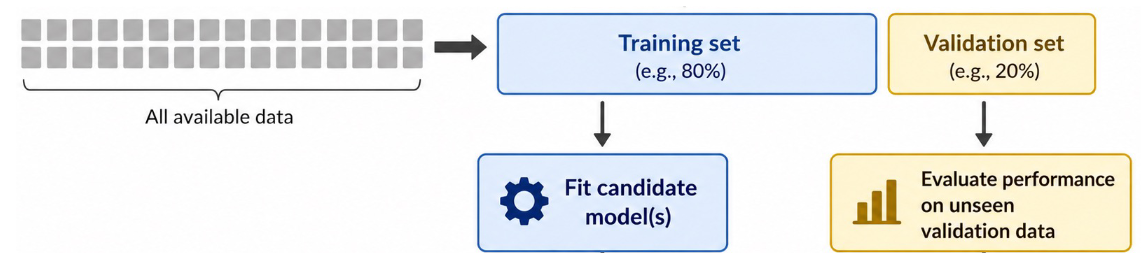
\includegraphics[width=0.5\linewidth]{img//model_selection/train_test_split.png}
\end{figure}\hfill\\
Thanks to the fact the observations in the dataset are different datapoints, this metric si better in evaluating our model with respect to $\widehat{Err}_{train}$: training erro is typically optimistically biased, especially with very flexible models.
\begin{figure}[h]
    \centering
    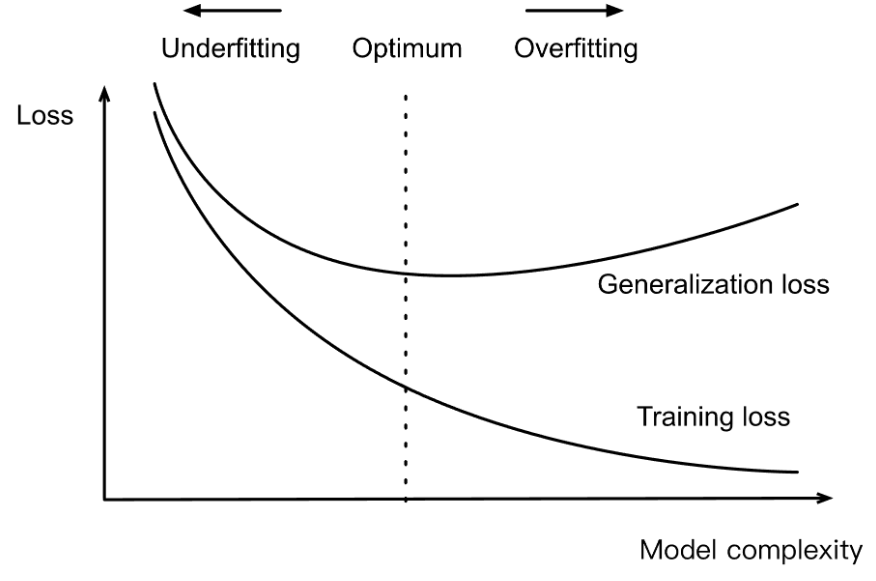
\includegraphics[width=0.4\linewidth]{img//model_selection/train_test_error_comparison.png}
\end{figure}

\vspace{0.2cm}
However this approach is not prefect: if we get unlucky the result of the validation set might be highly biased by the division, and we are "wasting" some data that could potentially be used for training a better model.

\newpage
\subsection{K-fold Cross-Validation (CV)}
The idea is to split the whole data in \textbf{k-folds} $\mathcal{D}= \mathcal{D}_1,\mathcal{D}_2\ ...\mathcal{D}_K $ and $\forall$  fold $k$ train the model on the remaining folds and test it on $\mathcal{D}_k$.At the end we validate the model on the \textbf{cross-validation estimate} \textcolor{gray}{(just the average of all fold's misprediction error)}:
$$
CV_K = \frac{1}{K}\sum_{k=1}^{K} \frac{1}{|D_k|}\sum_{i \in D_k} L(y_i, \hat{f}^{(-k)}(x_i))
$$
\begin{figure}[h]
    \centering
    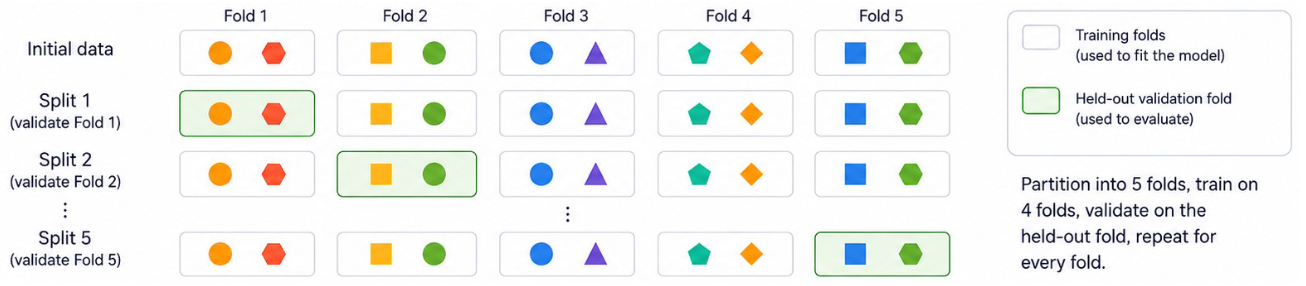
\includegraphics[width=0.8\linewidth]{img//model_selection/cross_validation.png}
\end{figure}

\vspace{0.2cm}
\textbf{Note}: cross-validation can be used both for \textit{model assessment} (how well my model generalize the data, evaluating the model on the CV) and \textit{model selection} (which model shoudl we choose, choosing the model that minimizes the CV error)
\vspace{0.2cm}

The cross-validation technique allows us to visualize the \textbf{overfitting} problem: the more the model overfits the more the CV error increases w.r.t. training error.
\begin{figure}[h]
    \centering
    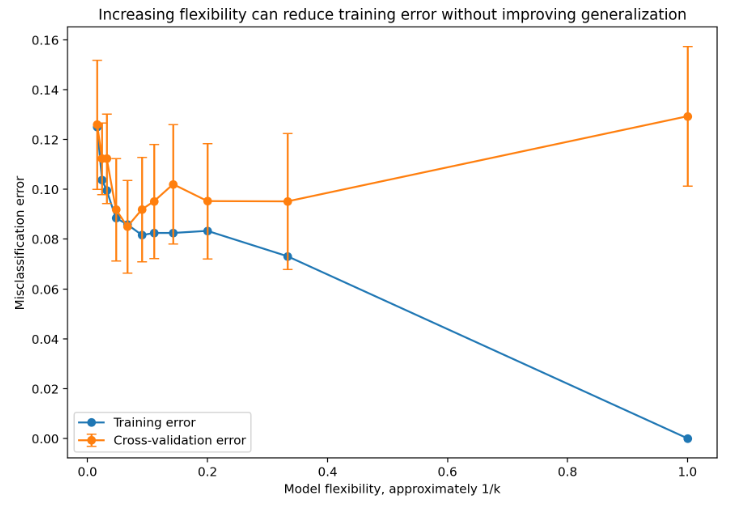
\includegraphics[width=0.5\linewidth]{img//model_selection/overfitting_visualized.png}
\end{figure}
\vspace{0.2cm}
Another thing worth of beding visualized is the mean and the std deviation of the error across different folds, in order to get an idea of the CV variability (however these are not CIs since the sets are not indepenent).
\begin{figure}[h]
    \centering
    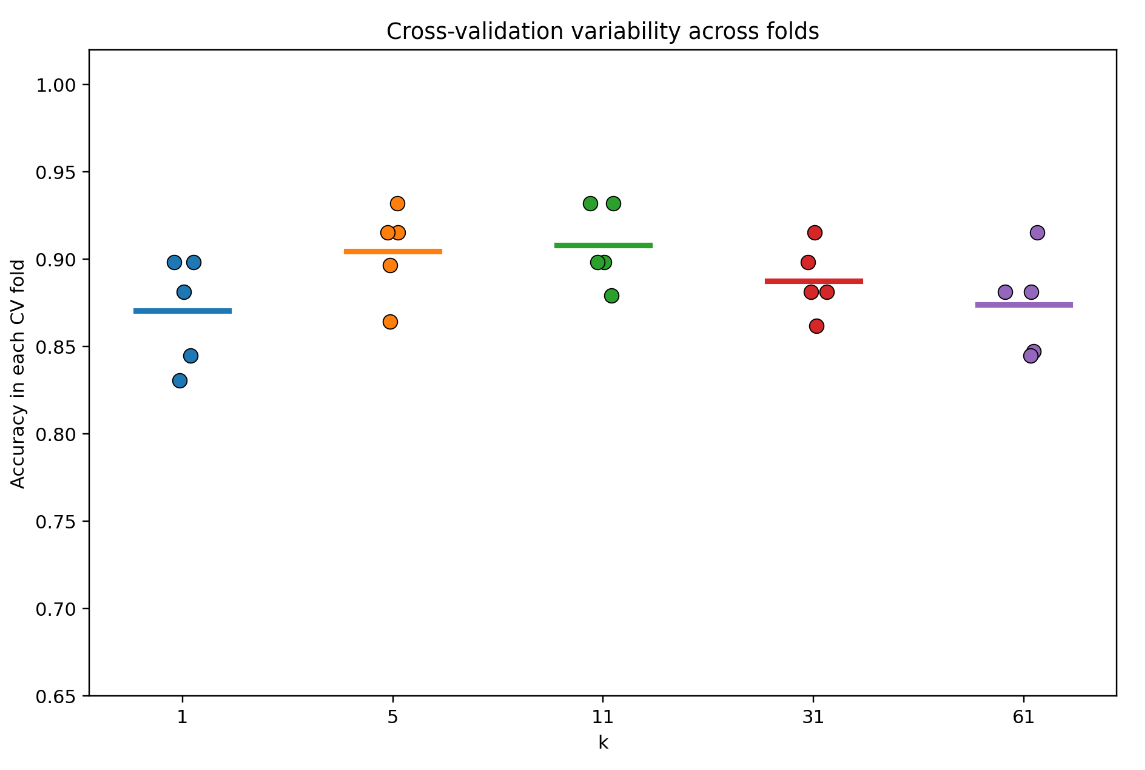
\includegraphics[width=0.5\linewidth]{img//model_selection/cv_variability.png}
\end{figure}

\subsection{Bootstrapping}
CV helps understanding the goodness of our model in generalizing data and might help in choosing the hyperparameters. However usually we'd like to understand \textit{how variable/stable is our result}.
\vspace{0.2cm}
The idea is to use our dataset as population and simulate a new "dataset" by sampling from it \textcolor{gray}{(this method is used also outside the supervised learning framework)}.
\begin{enumerate}
    \item we sample with replacement $n$ observations from \dataset: $\mathcal{D}^{*b}=\{z_1^{*b}...z_n^{*b}\}$:= \textbf{boostrap sample} for $b=1...B$ 
    \item compute some statistic (any kind) on the boostrap sample $\hat{\theta}^{*b}=s(\mathcal{D}^{*b})$
    \item we use the distribution of the statistics $\hat{\theta}^{*1}...\hat{\theta}^{*B}$ to estimate that uncertanty, like uncertanty intervals \arrow for example we can build percentile intervals $[q_{0.025}(\hat{\theta}^*),q_{0.975}(\hat{\theta}^*)]$
\end{enumerate}

In supervised learning we use the boostraping to fit a model $\hat{f}^{*b}()$ on each boostrap sample $\mathcal{D}^{*b}$ (each data sampled is a pair $(x_i,y_i)$, allowing us to verify several quantities across different models:\\
\begin{itemize}
    \item we can check the \textbf{variability of the model parameters} of the regression coefficients $\hat{\beta}_j^{*1}...\hat{\beta}_j^{*B}$
    \item we can check for the \textbf{variability of the prediction} $\hat{f}^{*1}(x_0)...\hat{f}^{*B}(x_0)$ on a fixed point $x_0$
    \item we can check the \textbf{variability of the model performance}
\end{itemize}
For example in \textit{KNN} we can use to bootstrap both to check the stability of the parameter $k$, to check the stability of the AUC or even to check the stability of the predictors.\\
\vspace{0.3cm}
The replacement in the bootstraping is essetial, but causes some observations to never been selected. Given $n$ observations, we have that the probabilityof each observation of not bein selected is:
$$
\left(1-\cfrac{1}{n}\right)^n\approx e^{-1}\approx 0.368
$$
the set of observations left-out is called the \textbf{out-of-bag} observations.
\begin{figure}[h]
    \centering
    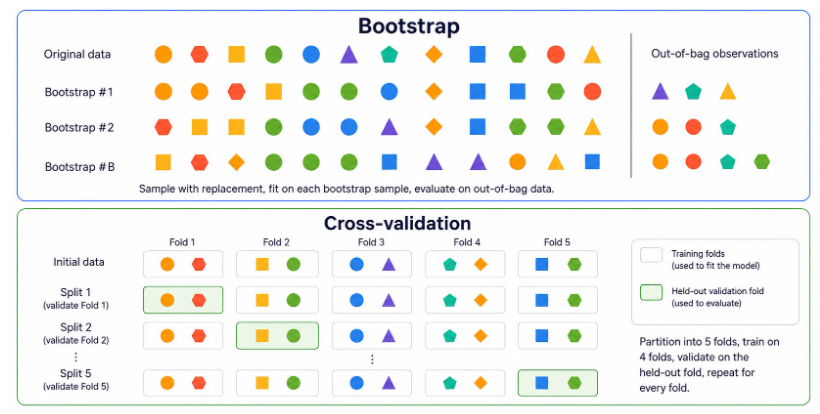
\includegraphics[width=0.7\linewidth]{img//model_selection/boostrap_example.png}
\end{figure}
\section{Feature selection}
So far we've dealt only with the complexity of the model, but what about the features? 
We'd like to select only those features that are more relevant in order to have the right quality and quantity. The idea of starting from a full-model $\mathcal{M}_{\text{all}} = \{x_1, x_2, \ldots, x_p\}$ we want to derive a \textbf{selected-feature model} $\mathcal{M}_S = \{x_j : j \in S\}, S \subseteq \{1, \ldots, p\}$ with the \textit{the best balanca between prediction accuracy and complexity}.

\begin{figure}[h]
    \centering
    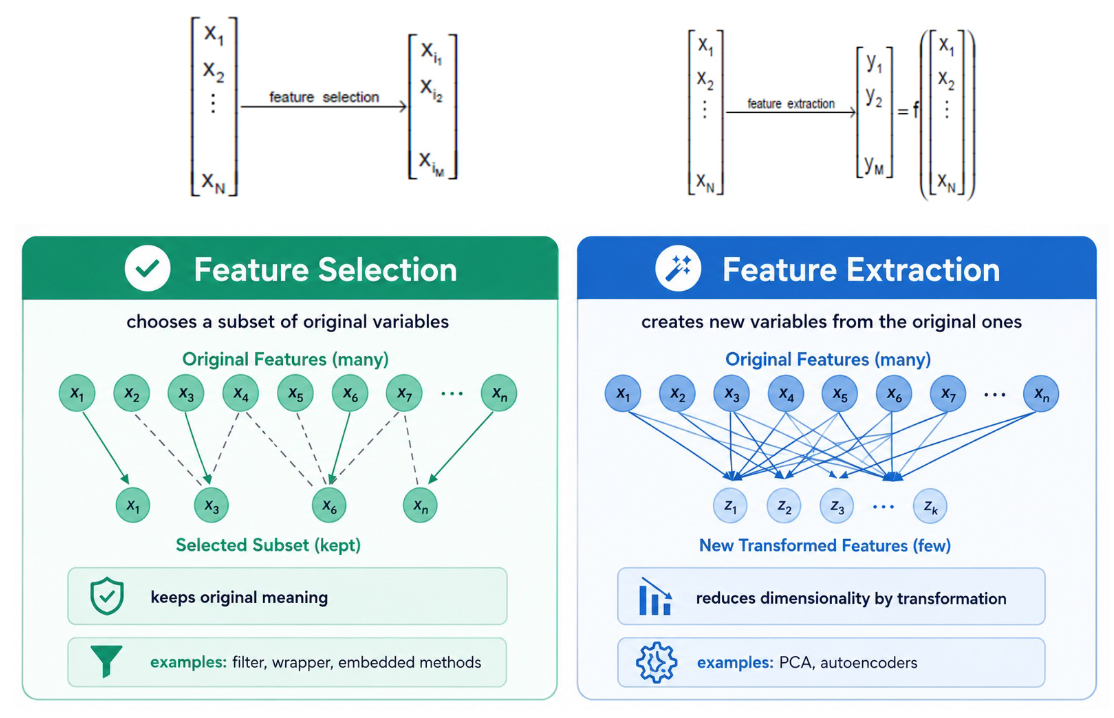
\includegraphics[width=0.7\linewidth]{img//feature_selection/feature_selection_vs_extraction.png}
    \caption*{Feature selection is different from feature extraction moethods like PCA: here we want only to select those features among those already present.}
\end{figure}

\subsection{Filter methods}
In this class of methods we rank the features following some metric that doesn't depend on the actual model and we pick only the top ones.\\
\begin{figure}[h]
    \centering
    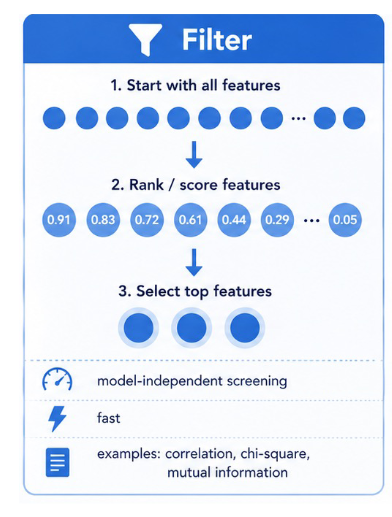
\includegraphics[width=0.3\linewidth]{img//feature_selection/filter_summary.png}
\end{figure}

Examples of scoring metrics \textcolor{gray}{(just examples, you don't need to know them)}:
\begin{itemize}
    \item correlation with the outcome;
    \item t-test / ANOVA;
    \item chi-square test for categorical features;
    \item mutual information;
    \item variance threshold;
    \item univariate logistic regression p-values.
\end{itemize}

\begin{minipage}[t]{0.45\textwidth}
  \textcolor{green!60!black}{\textbf{Pros:}}
  \begin{itemize}
    \item very simple
    \item very fast
    \item useful when $p$ is large
  \end{itemize}
\end{minipage}
\begin{minipage}[t]{0.45\textwidth}
  \textcolor{red}{\textbf{Cons:}}
  \begin{itemize}
    \item usually considers features one at a time;
    \item may miss interactions;
    \item may keep redundant variables;
    \item does not directly optimize predictive performance.
  \end{itemize}
\end{minipage}

\subsubsection{Multivariate Filering}
With this family of algorithms each feature based on the other selected: $score(x_j,Y,S)$ where $Y$ are the outcomes and $S$ are the selected features.\\
\vspace{0.2cm}
One metric used is the \textbf{minimum Redundancy Maximum Relevance (MRMR)} which selects the features balancing the relevance fo the single feture for $Y$ and the low redundancy of the features.
$$
\text{score}(x_j) = I(x_j; Y) - \frac{1}{|S|}\sum_{x_k \in S} I(x_j; x_k)
$$
where $I(x_j; Y)$ := relevance of the feature for the score, $I(x_j; x_k)$ := redundant information within features.

wrapper : select the fatures that give the best performance for my model (basically choose those features that give the best result for my model,I pick what's better for me)
embedded: do both feature selection and model selection at the same time.

\subsection{Wrapper methods}
In this class of methods we select those features giving the best result for our model, so these are \textbf{model-dependent} algorithms and are often used together with cross-validation to select the subsets.
$$
S^*=\arg\max_S\ CV(\ \text{perf}(S)\ )
$$
\begin{figure}[h!]
    \centering
    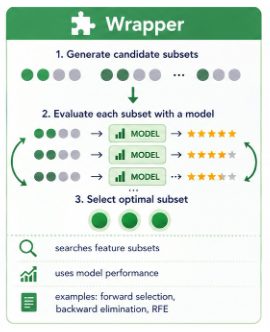
\includegraphics[width=0.3\linewidth]{img//feature_selection/wrapper_methods.png}
\end{figure}
\newpage

\begin{minipage}[t]{0.45\textwidth}
  \textcolor{green!60!black}{\textbf{Pros:}}
    \begin{itemize}
        \item directly bounded to model performance
        \item they'reable to capture fatires interactions
    \end{itemize}
\end{minipage}
\begin{minipage}[t]{0.45\textwidth}
    \textcolor{red}{\textbf{Cons:}}
    \begin{itemize}
        \item computational expensive
        \item may overfit, need careful cross-validation
    \end{itemize}
\end{minipage}
    
\subsubsection{Forward selection}
Start with no features and one at a time, verifying if by adding it the model performance improve. This type of methods is useful when only a small subset of features is relevant in a large number of predictors.
\subsubsection{Backward elimination}
Start with all the features and remove it one at a time. We choose the feature to remove based on which causes the minor loss in model performance. Useful to simplify the model when it's easy to fit.
\subsubsection{Recursive Feature Elimination (RFE)}
Start with all features, fit a model, rank features by model-based importance, remove the weakest feature or features, and repeat. Useful when the model gives some feature importance score, like the coefficients in linear regression.

\subsection{Embedded methods}
With embedded methods we embedd the feature selection directly into the learning algorithm, allowing it to determining automatically which features are more important.\\ 
The two main methods are \textbf{coefficient shrinkage} in which we try to shrink down a coefficient to zero, and \textbf{feature importance} (see later).\\
\begin{figure}[h]
    \centering
    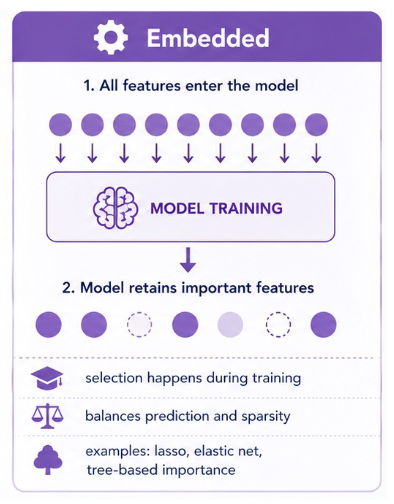
\includegraphics[width=0.3\linewidth]{img//feature_selection/embedded_methods.png}
\end{figure}
\textcolor{green!60!black}{\textbf{Pros:}}
\begin{itemize}
    \item computationally efficient since we train the model only once
    \item the are able to capture interaction betwwen the model and the features
    \item allow to reduce overfitting by focusing only on the most relevant features
\end{itemize}
\newpage
\subsection{Regularization}
If we take in consideration a std linear predictor $\eta(x)=\beta_0+\beta_1x_1...+\beta_px_p$ in general we have that the coefficients become unstable when $p$ is large. The idea of regularization is to \textbf{modify the fitting objective} in order to penalize the model complexity \arrow  we add a bias to favor the selection of simpler models.
$$
\text{Loss}(\beta) +\lambda\cdot\text{penalty}(\beta)\quad \lambda:=\text{regulatization strength}\ge 0
$$

By doing so we can't intepret easily the coefficient as in std regression, so to obtain an interpretable model we can run the regularization, select the most important/relevant features and re-fit the model only on those.

\subsubsection{Ridge regression}
As penaly we use the square of the coefficients, $L_2$. By doing so the coefficients will go toward zero (but not zero) as we set a stronger $\lambda$  and keeps in the model all the variables. It also helps with correlated predictors and reduce model variance. However it never preforms a feature selection 'cause coefficients are never drawn to zero, they only become very small, so it's not strictly an embedded feature selection method.
$$
L_2=\lambda\sum_{j=1}^p\beta_j^2
$$
\begin{figure}[h]
    \centering
    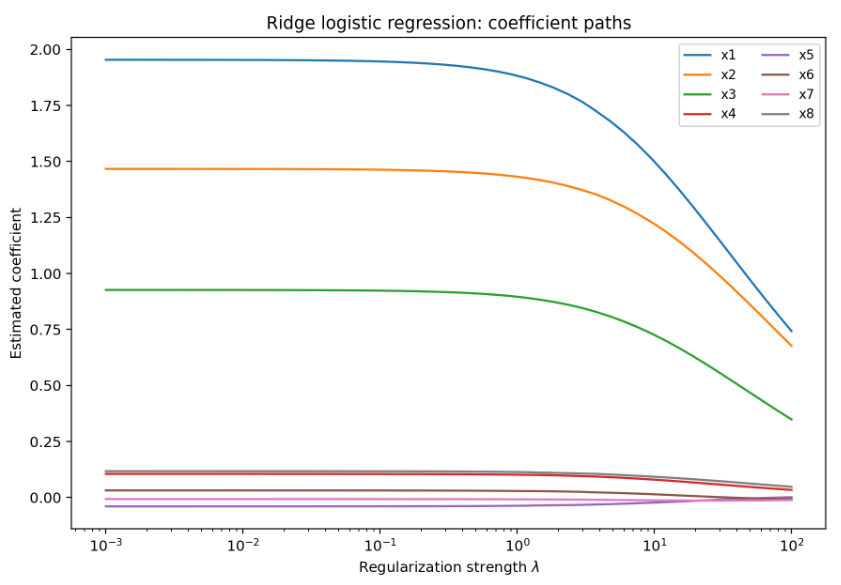
\includegraphics[width=0.4\linewidth]{img//feature_selection/ridge_regression.png}
\end{figure}

\subsubsection{Least Absolute Shrinkage and Selection Operato (LASSO) regression}
Here instead we use the $L_1$ penalty. Using this penalty function allows us to shrink coefficient down to zero, performing de facto embedded feature selection along with regularization.
$$
L_1=\sum_{j=1}^p|\beta_j|
$$
\begin{figure}[h]
    \centering
    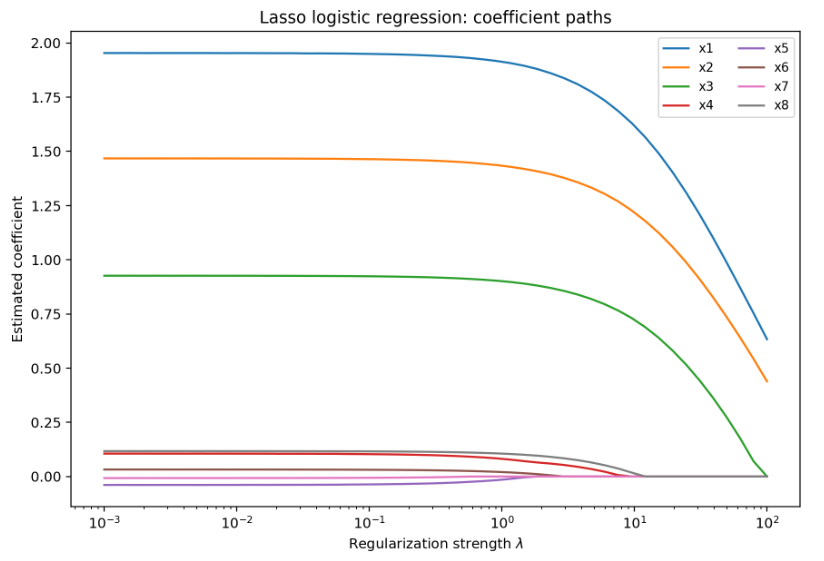
\includegraphics[width=0.4\linewidth]{img//feature_selection/lasso.png}
\end{figure}

\vspace{0.2cm}
Due the ability of shrinking coefficient up to 0 LASSO migh produce \textbf{sparse models} := models in which some original features are excluded (in other words, the coefficients are zero). The produced models are more sparse as $\lambda$ increases, so the regulatization strength controls both the shrinkage and the number of selected features.\\
\begin{figure}[h]
    \centering
    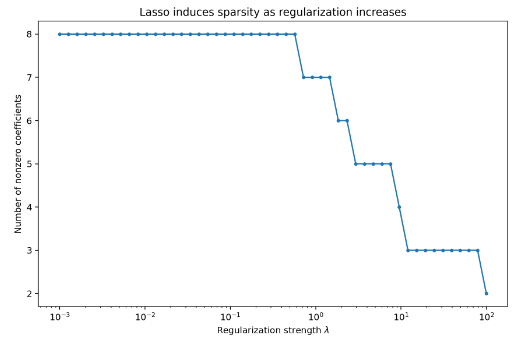
\includegraphics[width=0.4\linewidth]{img//feature_selection/lasso_sparse_model.png}
\end{figure}
However with LASSO we can't choose which coefficient are shrink to 0.\\

How do we choose the right $\lambda$? We use validation/cross-validation.
$$
\hat{\lambda}=\arg\max_\lambda\ CV_{performance}(\lambda)
$$
\begin{figure}[h]
    \centering
    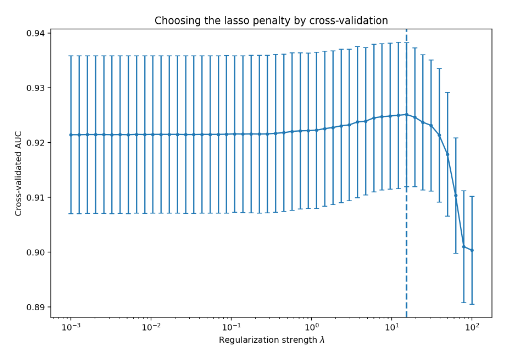
\includegraphics[width=0.4\linewidth]{img//feature_selection/reg_choosing_strength.png}
\end{figure}

What happens when there are two strongly correlated predictors?\\
\begin{description}
    \item[Ridge] tends to distribute the weight across correlated predictors
    \item[LASSO] tends to choose on predictor and shrinking it more rapidly than the other one
    \arrow this means that LASSO might be unstable when predictors are highly correlated
\end{description}
\begin{figure}[h]
    \centering
    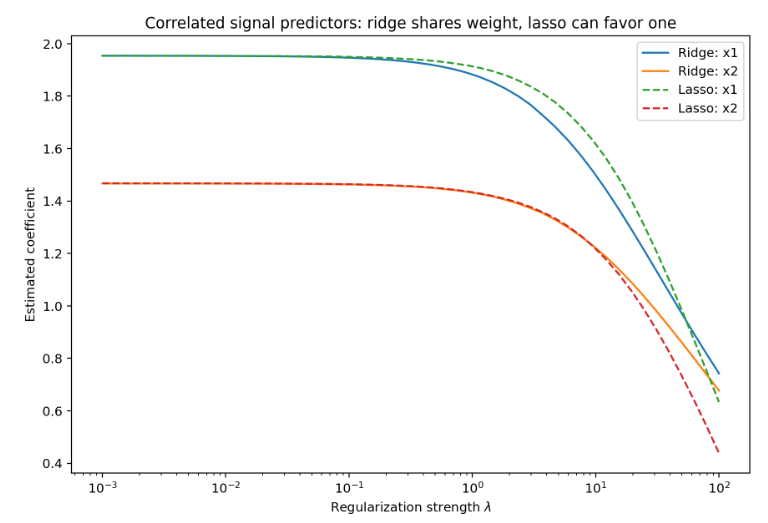
\includegraphics[width=0.4\linewidth]{img//feature_selection/lasso_stability.png}
\end{figure}
So in order to have a clearer idea we should run LASSO several times and compare the results: if some feature remain consistently revalant across all runs, then it's probably very relevant. Thereofre LASSO can be used also to exploit collinearity. 
\section{Data Leakage}
This problem arises when some informaton in the validation set influences the training 
datase: the model isn't working with two independent sets. This lead to optimistic performance estimations, by which the model looks better than in reality.\\
\vspace{0.2cm}
This leakage might happen in a lot of situations, but they all have a common denominator: all has to be executed on the training data, not on the validation set, otherwise we have leakage.
\begin{itemize}
    \item scaling/standardization
    \item feature selection
    \item shrinkage/regularization
    \item PCA/feature extraction
    \item preprocessing
\end{itemize}
\begin{figure}[h]
    \centering
    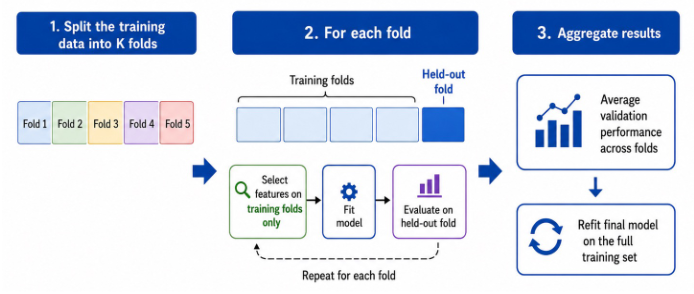
\includegraphics[width=0.75\linewidth]{img/data_leak_splitting.png}
    \caption{The splitting isn't something trivial.}
\end{figure}
\section{Decision-tree methods}
This methods don't rely on any assumption on the data, they just try to split the space to obtain the best classification/regression possible. To do that it splits the predictor space in regions $R_1,R_2...R_M$ and the prediction for each region is the mean of the datapoints in it.
$$
\hat{y}_{R_m} = \frac{1}{|R_m|} \sum_{i: x_i \in R_m} y_i
$$
\begin{figure}[h]
    \centering
    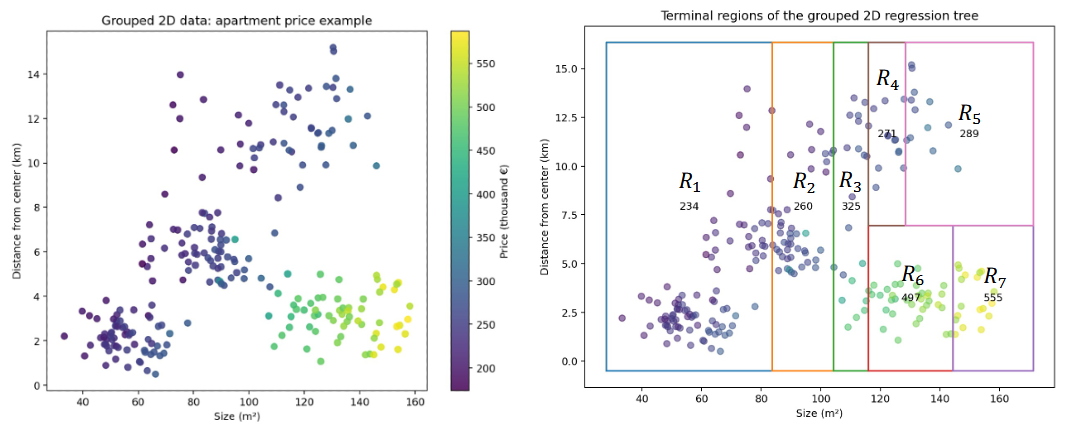
\includegraphics[width=0.75\linewidth]{img//tree-models//decision-tree/decision_tree.png}
\end{figure}
\begin{figure}[h]
    \centering
    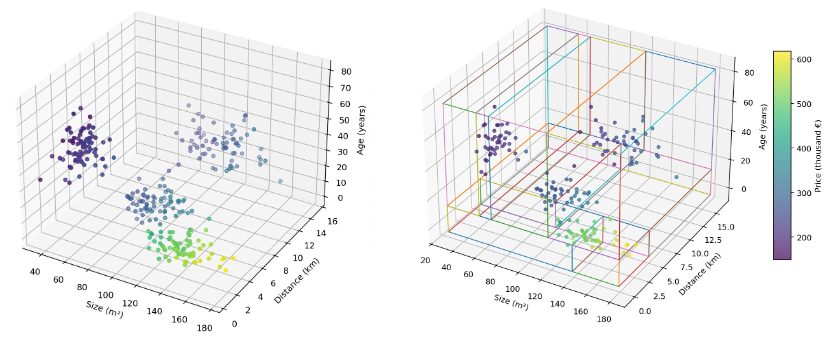
\includegraphics[width=0.75\linewidth]{img//tree-models//decision-tree/decision_tree_3d.png}
\end{figure}
The splits are \textit{axis-align}: all the splits are the type of $R_s\le s$, allwoing us to dividing the space only hyperplanes. However the non-linearity and complex splits arise from the interaction of \diff splits\textcolor{gray}{(think about the geometry of optimization problems in FOR)}.\\
\newpage
It's called a \textbf{piecewise-constant model} 'cause the predition is a sort of step function with a finite set of values as prediction.
\begin{figure}[h]
    \centering
    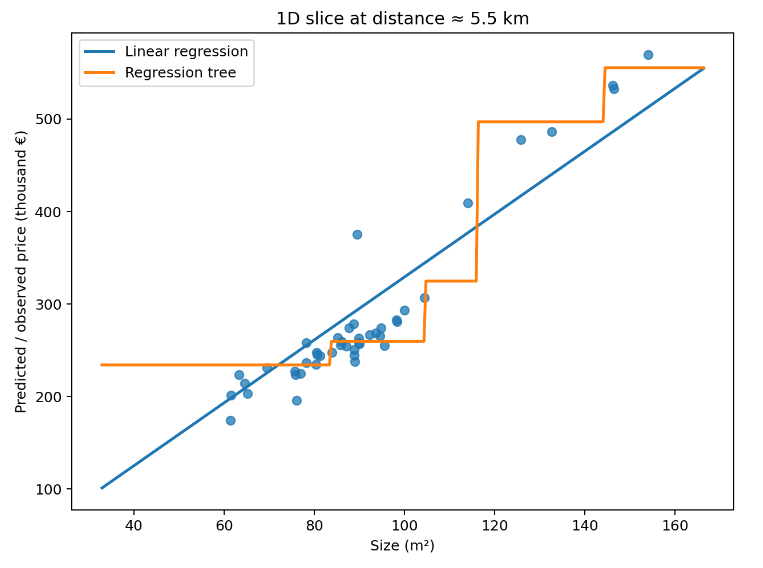
\includegraphics[width=0.3\linewidth]{img//tree-models//decision-tree/dectree_prediction_line.png}
\end{figure}

The same function can be described equivalently using binary trees:
\begin{figure}[h]
    \centering
    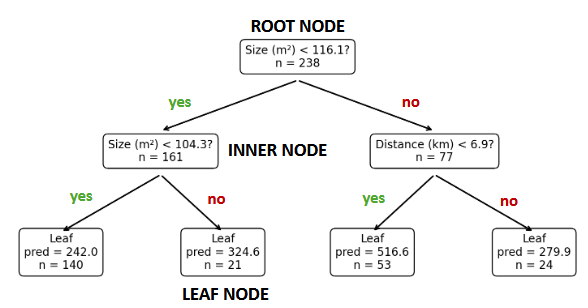
\includegraphics[width=0.4\linewidth]{img//tree-models//decision-tree/decision_tree_mathmodel.png}
\end{figure}\hfill\\
For what concerns \textbf{classification} each leaf node predicts $\hat{y}=\text{majority class}$ and we can estimate $\mathbb{P}(Y=\hat{y}|X\in R_m)=\# \text{ class }\hat{y}\ / \#\text{ total observations }$.


\subsection{Regression tree-fit: binary splitting}
As usual the goal is to minimize the RSS error:
$$
\text{RSS} = \sum_{j=1}^{J} \sum_{i \in R_j} (y_i - \hat{y}_{R_j})^2
$$
however doing so requires to try out all the possible combos of splitting, which is unfeasible \arrow we have to approach the problem using a top-down, greedy algorithm known as \textbf{recursive binary splitting}.
\vspace{0.2cm}
At each step we choose a predictor, we take all the possible thresholds and we select the one that gives us the largest reduction in prediction error:
$$
(j^*, s^*) = \arg\min_{j,s} \text{RSS}(j,s) = \arg\min_{j,s}\sum_{x_{x_i} \in R_L(j,s)} (y_i - \bar{y}_{R_L})^2 + \sum_{x_{x_i} \in R_R(j,s)} (y_i - \bar{y}_{R_R})^2
$$
\begin{figure}[h]
    \centering
    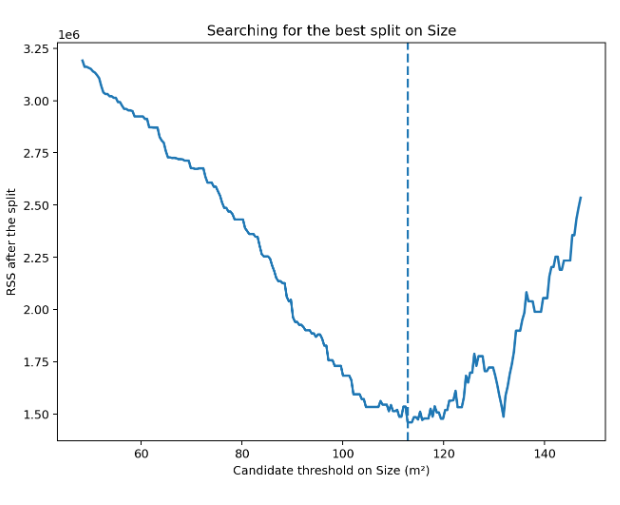
\includegraphics[width=0.35\linewidth]{img//tree-models//decision-tree/dectree_threshold_selection.png}
\end{figure}
\newpage
Technically we can continue forever with the splitting, but when do we stop? There are several criterions:
\begin{itemize}
    \item min num of obs required to split: $|R_m|<n_{min}^{split}$ 
    \item min num of obs allowed in each terminal node \textcolor{gray}{(dont't do the split if I end up with something too small)}: $|R_L|<n_{min}^{leaf},\ \  |R_R|<n_{min}^{leaf}$
    \item max tree depth: $depth(R_m)\ge d_{max}$
    \item min improvement: $\max_{j,s} \Delta \text{RSS}(j,s) = \max_{j,s} \text{RSS}(R_m) - [\text{RSS}(R_L(j,s)) + \text{RSS}(R_R(j,s))] < \varepsilon$ 
\end{itemize}

\subsection{Decision-tree complexity control}
As in all the models, we have to controll the complexity 'cause as the number of leaf increases the validation error might increase. The idea is to build the tree as far as our stopping criterion allows us, and then we trim some leafs.

\subsubsection{Cost-complexity pruning}
The goal is to minimize not only the erro but also the number of leafs ($\alpha$ is an hyperparam and it's selected using cross-validation):\\
$$
\text{RSS}(T)+\alpha |T|\quad |T| := \text{num terminal nodes}
$$
\vspace{0.2cm}
Then we start from a large tree $T_0$ we generate a sequence of sub-trees $T_0 \supset T_1 \supset T_2 \supset \cdots \supset T_L$ as follows: for each internal node $t$ consider the sub-tree rooted in it $T_t$, then compute the RSS by keeping that subtree and the RSS by removing it, and compute the following, choosing the lowest one.
$$
g(t) = \frac{RSS(t)-RSS(T_t)}{|\bar{T_t}|-1} := \text{pruning cost per leaf removed}
$$
\begin{figure}[h]
    \centering
    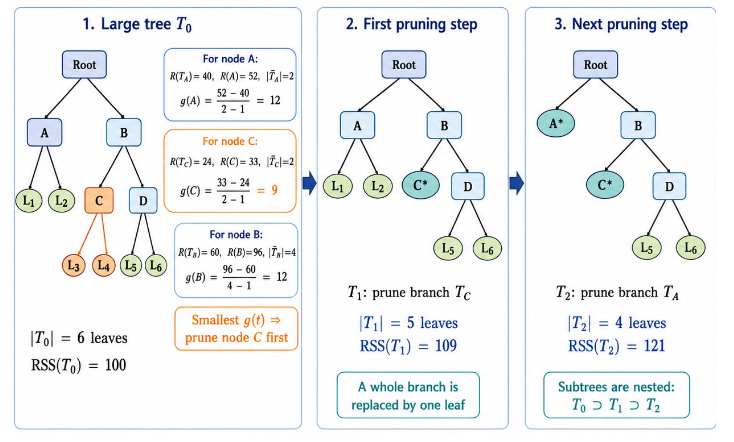
\includegraphics[width=0.75\linewidth]{img//tree-models//decision-tree/cost_complexity_pruning.png}
\end{figure}

\newpage
Each of the trees obtained is optimal for some range of $\alpha$ for the cost-complexity metric:
\begin{figure}[h]
    \centering
    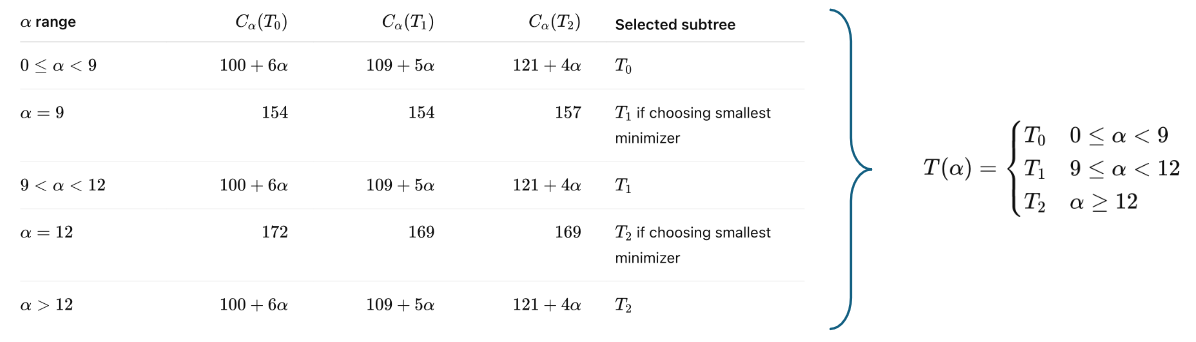
\includegraphics[width=0.75\linewidth]{img//tree-models//decision-tree/alpha_selection.png}
\end{figure}\hfill\\
and in the end we select using cross-validation $\hat{\alpha}=\arg\min_{\alpha}CV(\alpha)$, choosing the subtree among the candidate pruned subtrees for that $\alpha$ value.

\vspace{0.3cm}
\subsubsection{Feature selection using decision trees}
Trees can be used also for selecting relevant features: during the branch construction only some variables are used, so if a predictor never appears in a split it means it doesn't contribute to the prediction. However the variable selection might be unstable, so we have to select the predictors based on some average execution.
\begin{figure}[h]
    \centering
    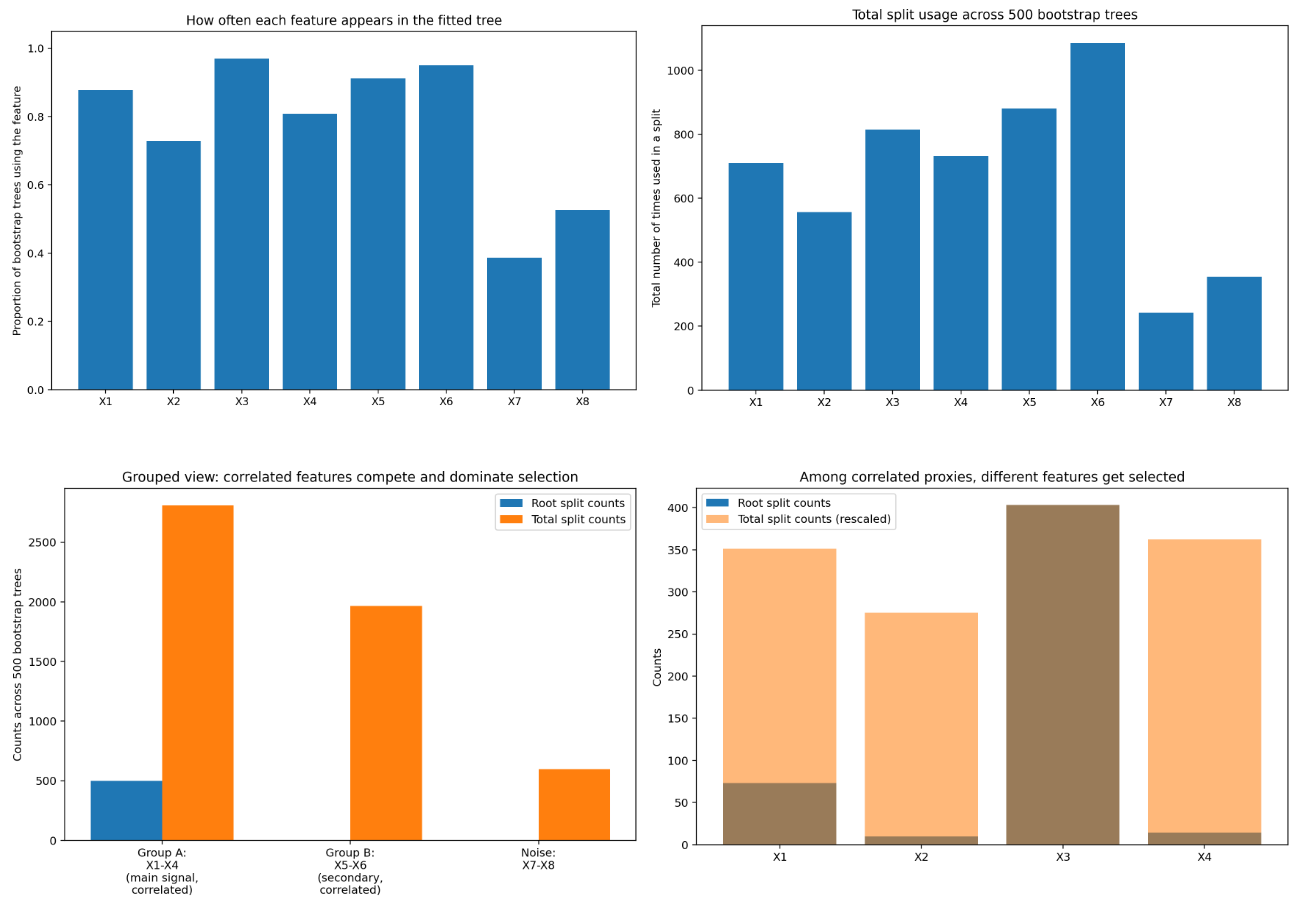
\includegraphics[width=0.85\linewidth]{img//tree-models//decision-tree/dectree_feature_selection.png}
\end{figure}

\subsubsection{Pro \& Cons: decision trees}
\begin{minipage}[t]{0.45\textwidth}
\textcolor{green}{\textbf{Pro:}}
\begin{itemize}
    \item are easy to explain
    \item produce if-then rules
    \item handle nonlinear effects
    \item capture interactions automatically
    \item do not require feature scaling \textcolor{gray}{(they handle one predictor at a time)}
    \item can handle numerical and categorical predictors
    \item can handle missing values \textcolor{gray}{(prediction are arranged base on the avrage)}
    \item perform a form of embedded feature selection
\end{itemize}
\end{minipage}
\begin{minipage}[t]{0.45\textwidth}
\textcolor{red}{\textbf{Cons:}}
\begin{itemize}
    \item can overfit
    \item are high-variance
    \item may be unstable
    \item produce stepwise predictions
    \item can be sensitive to small changes in the training data
\end{itemize}
\end{minipage}

\end{document}